\documentclass[11pt,twoside, authoryear]{elsarticle}
\usepackage[frenchb, english]{babel}
\usepackage[utf8]{inputenc}
%\usepackage[utf8]{fontenc}
%\usepackage[ansinew]{inputenc}
\usepackage{setspace}
\usepackage{babel,varioref}
\usepackage{supertabular}
\usepackage{graphicx}
%\usepackage[pdftex]{graphicx}
%\DeclareGraphicsExtensions{.pdf,.mps,.png,.jpg,.eps}
\usepackage{lscape}
\usepackage[authoryear]{natbib}
%\usepackage[frenchb,english]{babel}
\usepackage{multirow}
\usepackage{ifthen}
%\usepackage{harvard}
\usepackage{vmargin}
\usepackage{verbatim}
\usepackage{array}
%\usepackage[authoryear]{natbib}
\usepackage{hyperref}
\hypersetup{colorlinks=true,linkcolor=Black, citecolor=blue, urlcolor=blue}
%\setmarginsrb{2cm}{2cm}{2cm}{2cm}{0cm}{0cm}{0cm}{0cm}
\usepackage{booktabs,caption,fixltx2e}

\usepackage[flushleft]{threeparttable}

%\usepackage{titling}

%\setlength{\droptitle}{-10em}   % This is your set screw


\makeatletter
\def\ps@pprintTitle{%
  \let\@oddhead\@empty
  \let\@evenhead\@empty
  \let\@oddfoot\@empty
  \let\@evenfoot\@oddfoot
}
\makeatother
\usepackage{adjustbox}
\usepackage{chngcntr}
\counterwithin{table}{section}
%\usepackage[round]{natbib}

\renewcommand{\thesection}{\Alph{section}}

% \newcommand\section[1]{%
%   \refstepcounter{section}%
%   \addcontentsline{toc}{section}{\protect\numberline{\thesection}#1}%
%   \sectionmark{#1}}
%   }


% % \refstepcounter{section}%
% %   \addcontentsline{toc}{section}{\protect\numberline{\thesection}#1}%
% %   \sectionmark{#1}}



%   \newcommand\subsection[1]{%
%   \refstepcounter{subsection}%
%   \addcontentsline{toc}{subsection}{\protect\numberline{\thesubsection}#1}%
%   %\subsectionmark{#1}
%   }

%\EnableSectionsInLOFT



\begin{document}
\title{\textbf{International Transport costs:\\New Findings from modeling additive costs}\\Online Appendix (Not for Publication)}

\urlstyle{rm}

%\date{\vspace{-5ex}}

%Modèle additif seul DONE
%+Tableaux avec toutes les années en 3 digit DONE
% Tableaux avec toutes les années en 4 digit ???
%Harmoniser la présentation des résultats (cf table 1 du papier) DONE
%Les résultats sur la version Hummels mais avec sa pondération: en annexe du papier? En online appendix? DONE, mais à compléter


\maketitle





%\newpage

\tableofcontents
\vspace{1cm}
\newpage
\listoftables

\newpage



%
%
%
%
%			SECTION A / ADDITIVE ONLY
%			
%			
%				
%
%

	\renewcommand\thesubsubsection{\Alph{subsection}.\arabic{subsubsection}}
	
	\renewcommand\thesubsection{\Alph{subsection}}
	
	
\subsection{Three models: Comparison \label{secoa:additive_only}}

The paper compares the empirical performances of two models: one with only ad-valorem costs (Model (A)) and one with where both ad-valorem and additive costs (Model (B)).
In the interest of comprehensiveness,  we also estimate the model with only additive costs (Model (C)), in which case the estimated equation is:
$$\ln\left(\frac{p_{ik}}{\widetilde{p}_{ik}}-1 \right)= \ln \left(\frac{t_{i} + t_{s(k)}}{\widetilde{p}_{ik}}\right) + \epsilon^{add}_{ik}$$

This section is devoted to presenting the results. Precisely, we first compare the estimates of the transport costs components under the three models. In a second step, we report quality of fit tests for the three models.

\subsubsection{Estimation results}

In this section, we report the estimation results of the three models: Model (A) (with only ad-valorem costs), Model (B) (with both additive and ad-valorem) and Model (C) (with only additive costs). Table \ref{tab:3models_estimation_results_air} reports the results for air transport, Table \ref{tab:3models_estimation_results_ves} for vessel transport.

%%%% RAW TABLE TO BE FOUND AT: "...\Dropbox\Papier_Lise_Guillaume\trade_cost\results\3_models"
% modele iceberg tout seul : terme nlI
% colonnes L à U: modèle avec les deux
% termes nla, de V à Z, modèles avec que de l'additif
%nlI quer iceberg
%nla que additif
%nl : les deux
\setcounter{table}{0}
\renewcommand{\thetable}{A.\arabic{table}}


\begin{table}[htbp]
	\centering
	\footnotesize{
	\caption{Estimation results of the three models (Air, products at 5-digit level, sectors at 3-digit level)}
	\label{tab:3models_estimation_results_air}%
	\begin{tabular}{lllllll}
\cline{1-7}
\multicolumn{1}{c}{} &
  \multicolumn{1}{|r}{1974} &
  \multicolumn{1}{r}{1980} &
  \multicolumn{1}{r}{1990} &
  \multicolumn{1}{r}{2000} &
  \multicolumn{1}{r}{2010} &
  \multicolumn{1}{r}{2019} \\
\cline{1-7}
\multicolumn{1}{l}{\textbf{Data}} &
  \multicolumn{1}{|r}{} &
  \multicolumn{1}{r}{} &
  \multicolumn{1}{r}{} &
  \multicolumn{1}{r}{} &
  \multicolumn{1}{r}{} &
  \multicolumn{1}{r}{} \\
\multicolumn{1}{l}{\hspace{1em}{$\#$ obs.}} &
  \multicolumn{1}{|r}{14,955} &
  \multicolumn{1}{r}{16,118} &
  \multicolumn{1}{r}{24,958} &
  \multicolumn{1}{r}{35,027} &
  \multicolumn{1}{r}{40,284} &
  \multicolumn{1}{r}{44,133} \\
\multicolumn{1}{l}{\hspace{1em}{$\#$ sectors}} &
  \multicolumn{1}{|r}{203} &
  \multicolumn{1}{r}{204} &
  \multicolumn{1}{r}{212} &
  \multicolumn{1}{r}{218} &
  \multicolumn{1}{r}{216} &
  \multicolumn{1}{r}{218} \\
\multicolumn{1}{l}{\hspace{1em}{$\#$ origin countries}} &
  \multicolumn{1}{|r}{152} &
  \multicolumn{1}{r}{165} &
  \multicolumn{1}{r}{181} &
  \multicolumn{1}{r}{208} &
  \multicolumn{1}{r}{210} &
  \multicolumn{1}{r}{213} \\
\multicolumn{1}{l}{\hspace{1em}{\textit{Observed transport costs}}} &
  \multicolumn{1}{|r}{} &
  \multicolumn{1}{r}{} &
  \multicolumn{1}{r}{} &
  \multicolumn{1}{r}{} &
  \multicolumn{1}{r}{} &
  \multicolumn{1}{r}{} \\
\multicolumn{1}{l}{\hspace{2em}Mean (in $\%$)} &
  \multicolumn{1}{|r}{5.3} &
  \multicolumn{1}{r}{4.0} &
  \multicolumn{1}{r}{4.1} &
  \multicolumn{1}{r}{2.8} &
  \multicolumn{1}{r}{3.1} &
  \multicolumn{1}{r}{2.3} \\
\multicolumn{1}{l}{\hspace{2em}Median (in $\%$)} &
  \multicolumn{1}{|r}{3.3} &
  \multicolumn{1}{r}{1.6} &
  \multicolumn{1}{r}{1.9} &
  \multicolumn{1}{r}{1.4} &
  \multicolumn{1}{r}{1.9} &
  \multicolumn{1}{r}{1.6} \\
\multicolumn{1}{l}{\hspace{2em}Std. dev.} &
  \multicolumn{1}{|r}{6.7} &
  \multicolumn{1}{r}{6.4} &
  \multicolumn{1}{r}{6.0} &
  \multicolumn{1}{r}{4.8} &
  \multicolumn{1}{r}{5.2} &
  \multicolumn{1}{r}{3.6} \\
\multicolumn{1}{l}{{\textbf{Model (A)}}} &
  \multicolumn{1}{|r}{} &
  \multicolumn{1}{r}{} &
  \multicolumn{1}{r}{} &
  \multicolumn{1}{r}{} &
  \multicolumn{1}{r}{} &
  \multicolumn{1}{r}{} \\
\multicolumn{1}{l}{\hspace{1em}{\textit{Multiplicative term} ($\widehat{\tau}^{ice}-1$)}} &
  \multicolumn{1}{|r}{} &
  \multicolumn{1}{r}{} &
  \multicolumn{1}{r}{} &
  \multicolumn{1}{r}{} &
  \multicolumn{1}{r}{} &
  \multicolumn{1}{r}{} \\
\multicolumn{1}{l}{\hspace{2em}Mean (in $\%$)} &
  \multicolumn{1}{|r}{6.9} &
  \multicolumn{1}{r}{5.4} &
  \multicolumn{1}{r}{5.0} &
  \multicolumn{1}{r}{3.6} &
  \multicolumn{1}{r}{4.2} &
  \multicolumn{1}{r}{3.0} \\
\multicolumn{1}{l}{\hspace{2em}Median (in $\%$)} &
  \multicolumn{1}{|r}{5.4} &
  \multicolumn{1}{r}{3.8} &
  \multicolumn{1}{r}{4.4} &
  \multicolumn{1}{r}{2.5} &
  \multicolumn{1}{r}{3.4} &
  \multicolumn{1}{r}{2.6} \\
\multicolumn{1}{l}{\hspace{2em}Std. dev.} &
  \multicolumn{1}{|r}{5.2} &
  \multicolumn{1}{r}{4.9} &
  \multicolumn{1}{r}{3.9} &
  \multicolumn{1}{r}{3.3} &
  \multicolumn{1}{r}{3.7} &
  \multicolumn{1}{r}{2.3} \\
\multicolumn{1}{l}{{\textbf{Model (B)}}} &
  \multicolumn{1}{|r}{} &
  \multicolumn{1}{r}{} &
  \multicolumn{1}{r}{} &
  \multicolumn{1}{r}{} &
  \multicolumn{1}{r}{} &
  \multicolumn{1}{r}{} \\
\multicolumn{1}{l}{\hspace{1em}{\textit{Multiplicative term} ($\widehat{\tau}^{adv}-1$)}} &
  \multicolumn{1}{|r}{} &
  \multicolumn{1}{r}{} &
  \multicolumn{1}{r}{} &
  \multicolumn{1}{r}{} &
  \multicolumn{1}{r}{} &
  \multicolumn{1}{r}{} \\
\multicolumn{1}{l}{\hspace{2em}Mean (in $\%$)} &
  \multicolumn{1}{|r}{3.6} &
  \multicolumn{1}{r}{2.3} &
  \multicolumn{1}{r}{2.4} &
  \multicolumn{1}{r}{1.7} &
  \multicolumn{1}{r}{2.6} &
  \multicolumn{1}{r}{2.0} \\
\multicolumn{1}{l}{\hspace{2em}Median (in $\%$)} &
  \multicolumn{1}{|r}{2.7} &
  \multicolumn{1}{r}{1.6} &
  \multicolumn{1}{r}{1.6} &
  \multicolumn{1}{r}{1.2} &
  \multicolumn{1}{r}{2.2} &
  \multicolumn{1}{r}{1.8} \\
\multicolumn{1}{l}{\hspace{2em}Std. dev.} &
  \multicolumn{1}{|r}{3.2} &
  \multicolumn{1}{r}{2.5} &
  \multicolumn{1}{r}{2.1} &
  \multicolumn{1}{r}{1.6} &
  \multicolumn{1}{r}{2.3} &
  \multicolumn{1}{r}{1.5} \\
\multicolumn{1}{l}{\hspace{1em}{\textit{Additive term} ($\widehat{t}/\widetilde{p}$)}} &
  \multicolumn{1}{|r}{} &
  \multicolumn{1}{r}{} &
  \multicolumn{1}{r}{} &
  \multicolumn{1}{r}{} &
  \multicolumn{1}{r}{} &
  \multicolumn{1}{r}{} \\
\multicolumn{1}{l}{\hspace{2em}Mean (in $\%$)} &
  \multicolumn{1}{|r}{2.6} &
  \multicolumn{1}{r}{2.0} &
  \multicolumn{1}{r}{1.8} &
  \multicolumn{1}{r}{1.3} &
  \multicolumn{1}{r}{1.1} &
  \multicolumn{1}{r}{0.6} \\
\multicolumn{1}{l}{\hspace{2em}Median (in $\%$)} &
  \multicolumn{1}{|r}{1.1} &
  \multicolumn{1}{r}{0.5} &
  \multicolumn{1}{r}{0.8} &
  \multicolumn{1}{r}{0.5} &
  \multicolumn{1}{r}{0.4} &
  \multicolumn{1}{r}{0.3} \\
\multicolumn{1}{l}{\hspace{2em}Std. dev.} &
  \multicolumn{1}{|r}{4.0} &
  \multicolumn{1}{r}{4.1} &
  \multicolumn{1}{r}{3.3} &
  \multicolumn{1}{r}{2.8} &
  \multicolumn{1}{r}{2.4} &
  \multicolumn{1}{r}{1.7} \\
\multicolumn{1}{l}{\hspace{1em}{\textit{Share of additive costs} ($\widehat{\beta}$)}} &
  \multicolumn{1}{|r}{} &
  \multicolumn{1}{r}{} &
  \multicolumn{1}{r}{} &
  \multicolumn{1}{r}{} &
  \multicolumn{1}{r}{} &
  \multicolumn{1}{r}{} \\
\multicolumn{1}{l}{\hspace{2em}Mean (in $\%$)} &
  \multicolumn{1}{|r}{0.34} &
  \multicolumn{1}{r}{0.33} &
  \multicolumn{1}{r}{0.33} &
  \multicolumn{1}{r}{0.31} &
  \multicolumn{1}{r}{0.21} &
  \multicolumn{1}{r}{0.19} \\
\multicolumn{1}{l}{\hspace{2em}Median (in $\%$)} &
  \multicolumn{1}{|r}{0.30} &
  \multicolumn{1}{r}{0.28} &
  \multicolumn{1}{r}{0.29} &
  \multicolumn{1}{r}{0.30} &
  \multicolumn{1}{r}{0.18} &
  \multicolumn{1}{r}{0.13} \\
\multicolumn{1}{l}{\hspace{2em}Std. dev.} &
  \multicolumn{1}{|r}{0.24} &
  \multicolumn{1}{r}{0.23} &
  \multicolumn{1}{r}{0.21} &
  \multicolumn{1}{r}{0.20} &
  \multicolumn{1}{r}{0.18} &
  \multicolumn{1}{r}{0.19} \\
\multicolumn{1}{l}{{\textbf{Model (C)}}} &
  \multicolumn{1}{|r}{} &
  \multicolumn{1}{r}{} &
  \multicolumn{1}{r}{} &
  \multicolumn{1}{r}{} &
  \multicolumn{1}{r}{} &
  \multicolumn{1}{r}{} \\
\multicolumn{1}{l}{\hspace{1em}{\textit{Additive term} ($\widehat{t}^{add}/\widetilde{p}$)}} &
  \multicolumn{1}{|r}{} &
  \multicolumn{1}{r}{} &
  \multicolumn{1}{r}{} &
  \multicolumn{1}{r}{} &
  \multicolumn{1}{r}{} &
  \multicolumn{1}{r}{} \\
\multicolumn{1}{l}{\hspace{2em}Mean (in $\%$)} &
  \multicolumn{1}{|r}{6.9} &
  \multicolumn{1}{r}{4.8} &
  \multicolumn{1}{r}{4.4} &
  \multicolumn{1}{r}{3.1} &
  \multicolumn{1}{r}{4.4} &
  \multicolumn{1}{r}{2.9} \\
\multicolumn{1}{l}{\hspace{2em}Median (in $\%$)} &
  \multicolumn{1}{|r}{4.4} &
  \multicolumn{1}{r}{1.8} &
  \multicolumn{1}{r}{2.3} &
  \multicolumn{1}{r}{1.4} &
  \multicolumn{1}{r}{2.7} &
  \multicolumn{1}{r}{1.6} \\
\multicolumn{1}{l}{\hspace{2em}Std. dev.} &
  \multicolumn{1}{|r}{9.4} &
  \multicolumn{1}{r}{8.3} &
  \multicolumn{1}{r}{10.0} &
  \multicolumn{1}{r}{5.5} &
  \multicolumn{1}{r}{7.4} &
  \multicolumn{1}{r}{5.6} \\
\cline{1-7}
\end{tabular}

   \begin{tablenotes}
	\tiny
	\item Statistics are weighted by value
	\item \textbf{Model (A): Iceberg transport costs only}
	\item \textbf{Model (B): With additive and ad-valorem transport costs}
				\item \textbf{Model (C): With additive transport costs only}
\end{tablenotes}

}	
\end{table}%


\begin{table}[htbp]
	\centering
	\footnotesize{
		\caption{Estimation results of the three models (Vessel, products at 5-digit level, sectors at 3-digit level)}
		\label{tab:3models_estimation_results_ves}%
		\begin{tabular}{lllllll}
\cline{1-7}
\multicolumn{1}{c}{} &
  \multicolumn{1}{|r}{1974} &
  \multicolumn{1}{r}{1980} &
  \multicolumn{1}{r}{1990} &
  \multicolumn{1}{r}{2000} &
  \multicolumn{1}{r}{2010} &
  \multicolumn{1}{r}{2019} \\
\cline{1-7}
\multicolumn{1}{l}{\textbf{Data}} &
  \multicolumn{1}{|r}{} &
  \multicolumn{1}{r}{} &
  \multicolumn{1}{r}{} &
  \multicolumn{1}{r}{} &
  \multicolumn{1}{r}{} &
  \multicolumn{1}{r}{} \\
\multicolumn{1}{l}{\hspace{1em}{$\#$ obs.}} &
  \multicolumn{1}{|r}{19,007} &
  \multicolumn{1}{r}{17,356} &
  \multicolumn{1}{r}{28,383} &
  \multicolumn{1}{r}{36,093} &
  \multicolumn{1}{r}{37,748} &
  \multicolumn{1}{r}{41,137} \\
\multicolumn{1}{l}{\hspace{1em}{$\#$ sectors}} &
  \multicolumn{1}{|r}{239} &
  \multicolumn{1}{r}{232} &
  \multicolumn{1}{r}{232} &
  \multicolumn{1}{r}{230} &
  \multicolumn{1}{r}{226} &
  \multicolumn{1}{r}{223} \\
\multicolumn{1}{l}{\hspace{1em}{$\#$ origin countries}} &
  \multicolumn{1}{|r}{154} &
  \multicolumn{1}{r}{163} &
  \multicolumn{1}{r}{179} &
  \multicolumn{1}{r}{206} &
  \multicolumn{1}{r}{198} &
  \multicolumn{1}{r}{212} \\
\multicolumn{1}{l}{\hspace{1em}{\textit{Observed transport costs}}} &
  \multicolumn{1}{|r}{} &
  \multicolumn{1}{r}{} &
  \multicolumn{1}{r}{} &
  \multicolumn{1}{r}{} &
  \multicolumn{1}{r}{} &
  \multicolumn{1}{r}{} \\
\multicolumn{1}{l}{\hspace{2em}Mean (in $\%$)} &
  \multicolumn{1}{|r}{8.9} &
  \multicolumn{1}{r}{6.2} &
  \multicolumn{1}{r}{5.4} &
  \multicolumn{1}{r}{5.3} &
  \multicolumn{1}{r}{4.2} &
  \multicolumn{1}{r}{4.1} \\
\multicolumn{1}{l}{\hspace{2em}Median (in $\%$)} &
  \multicolumn{1}{|r}{7.3} &
  \multicolumn{1}{r}{4.9} &
  \multicolumn{1}{r}{4.1} &
  \multicolumn{1}{r}{4.3} &
  \multicolumn{1}{r}{3.2} &
  \multicolumn{1}{r}{3.0} \\
\multicolumn{1}{l}{\hspace{2em}Std. dev.} &
  \multicolumn{1}{|r}{6.7} &
  \multicolumn{1}{r}{5.0} &
  \multicolumn{1}{r}{4.8} &
  \multicolumn{1}{r}{4.7} &
  \multicolumn{1}{r}{3.6} &
  \multicolumn{1}{r}{3.5} \\
\multicolumn{1}{l}{{\textbf{Model (A)}}} &
  \multicolumn{1}{|r}{} &
  \multicolumn{1}{r}{} &
  \multicolumn{1}{r}{} &
  \multicolumn{1}{r}{} &
  \multicolumn{1}{r}{} &
  \multicolumn{1}{r}{} \\
\multicolumn{1}{l}{\hspace{1em}{\textit{Multiplicative term} ($\widehat{\tau}^{ice}-1$)}} &
  \multicolumn{1}{|r}{} &
  \multicolumn{1}{r}{} &
  \multicolumn{1}{r}{} &
  \multicolumn{1}{r}{} &
  \multicolumn{1}{r}{} &
  \multicolumn{1}{r}{} \\
\multicolumn{1}{l}{\hspace{2em}Mean (in $\%$)} &
  \multicolumn{1}{|r}{9.8} &
  \multicolumn{1}{r}{6.5} &
  \multicolumn{1}{r}{5.7} &
  \multicolumn{1}{r}{5.1} &
  \multicolumn{1}{r}{4.0} &
  \multicolumn{1}{r}{3.9} \\
\multicolumn{1}{l}{\hspace{2em}Median (in $\%$)} &
  \multicolumn{1}{|r}{9.6} &
  \multicolumn{1}{r}{5.5} &
  \multicolumn{1}{r}{4.6} &
  \multicolumn{1}{r}{4.8} &
  \multicolumn{1}{r}{3.5} &
  \multicolumn{1}{r}{3.8} \\
\multicolumn{1}{l}{\hspace{2em}Std. dev.} &
  \multicolumn{1}{|r}{5.3} &
  \multicolumn{1}{r}{4.0} &
  \multicolumn{1}{r}{3.2} &
  \multicolumn{1}{r}{2.8} &
  \multicolumn{1}{r}{2.0} &
  \multicolumn{1}{r}{1.7} \\
\multicolumn{1}{l}{{\textbf{Model (B)}}} &
  \multicolumn{1}{|r}{} &
  \multicolumn{1}{r}{} &
  \multicolumn{1}{r}{} &
  \multicolumn{1}{r}{} &
  \multicolumn{1}{r}{} &
  \multicolumn{1}{r}{} \\
\multicolumn{1}{l}{\hspace{1em}{\textit{Multiplicative term} ($\widehat{\tau}^{adv}-1$)}} &
  \multicolumn{1}{|r}{} &
  \multicolumn{1}{r}{} &
  \multicolumn{1}{r}{} &
  \multicolumn{1}{r}{} &
  \multicolumn{1}{r}{} &
  \multicolumn{1}{r}{} \\
\multicolumn{1}{l}{\hspace{2em}Mean (in $\%$)} &
  \multicolumn{1}{|r}{5.4} &
  \multicolumn{1}{r}{3.1} &
  \multicolumn{1}{r}{3.3} &
  \multicolumn{1}{r}{2.5} &
  \multicolumn{1}{r}{1.9} &
  \multicolumn{1}{r}{2.0} \\
\multicolumn{1}{l}{\hspace{2em}Median (in $\%$)} &
  \multicolumn{1}{|r}{4.9} &
  \multicolumn{1}{r}{2.4} &
  \multicolumn{1}{r}{2.8} &
  \multicolumn{1}{r}{2.1} &
  \multicolumn{1}{r}{1.8} &
  \multicolumn{1}{r}{1.7} \\
\multicolumn{1}{l}{\hspace{2em}Std. dev.} &
  \multicolumn{1}{|r}{4.1} &
  \multicolumn{1}{r}{2.3} &
  \multicolumn{1}{r}{2.2} &
  \multicolumn{1}{r}{2.1} &
  \multicolumn{1}{r}{1.7} &
  \multicolumn{1}{r}{1.4} \\
\multicolumn{1}{l}{\hspace{1em}{\textit{Additive term} ($\widehat{t}/\widetilde{p}$)}} &
  \multicolumn{1}{|r}{} &
  \multicolumn{1}{r}{} &
  \multicolumn{1}{r}{} &
  \multicolumn{1}{r}{} &
  \multicolumn{1}{r}{} &
  \multicolumn{1}{r}{} \\
\multicolumn{1}{l}{\hspace{2em}Mean (in $\%$)} &
  \multicolumn{1}{|r}{5.1} &
  \multicolumn{1}{r}{3.4} &
  \multicolumn{1}{r}{2.8} &
  \multicolumn{1}{r}{2.8} &
  \multicolumn{1}{r}{2.5} &
  \multicolumn{1}{r}{2.2} \\
\multicolumn{1}{l}{\hspace{2em}Median (in $\%$)} &
  \multicolumn{1}{|r}{2.9} &
  \multicolumn{1}{r}{2.3} &
  \multicolumn{1}{r}{1.7} &
  \multicolumn{1}{r}{2.2} &
  \multicolumn{1}{r}{1.9} &
  \multicolumn{1}{r}{1.8} \\
\multicolumn{1}{l}{\hspace{2em}Std. dev.} &
  \multicolumn{1}{|r}{8.5} &
  \multicolumn{1}{r}{4.6} &
  \multicolumn{1}{r}{4.1} &
  \multicolumn{1}{r}{4.3} &
  \multicolumn{1}{r}{2.5} &
  \multicolumn{1}{r}{2.3} \\
\multicolumn{1}{l}{\hspace{1em}{\textit{Share of additive costs} ($\widehat{\beta}$)}} &
  \multicolumn{1}{|r}{} &
  \multicolumn{1}{r}{} &
  \multicolumn{1}{r}{} &
  \multicolumn{1}{r}{} &
  \multicolumn{1}{r}{} &
  \multicolumn{1}{r}{} \\
\multicolumn{1}{l}{\hspace{2em}Mean (in $\%$)} &
  \multicolumn{1}{|r}{0.41} &
  \multicolumn{1}{r}{0.50} &
  \multicolumn{1}{r}{0.39} &
  \multicolumn{1}{r}{0.51} &
  \multicolumn{1}{r}{0.54} &
  \multicolumn{1}{r}{0.50} \\
\multicolumn{1}{l}{\hspace{2em}Median (in $\%$)} &
  \multicolumn{1}{|r}{0.38} &
  \multicolumn{1}{r}{0.51} &
  \multicolumn{1}{r}{0.38} &
  \multicolumn{1}{r}{0.48} &
  \multicolumn{1}{r}{0.53} &
  \multicolumn{1}{r}{0.47} \\
\multicolumn{1}{l}{\hspace{2em}Std. dev.} &
  \multicolumn{1}{|r}{0.30} &
  \multicolumn{1}{r}{0.25} &
  \multicolumn{1}{r}{0.21} &
  \multicolumn{1}{r}{0.28} &
  \multicolumn{1}{r}{0.30} &
  \multicolumn{1}{r}{0.25} \\
\multicolumn{1}{l}{{\textbf{Model (C)}}} &
  \multicolumn{1}{|r}{} &
  \multicolumn{1}{r}{} &
  \multicolumn{1}{r}{} &
  \multicolumn{1}{r}{} &
  \multicolumn{1}{r}{} &
  \multicolumn{1}{r}{} \\
\multicolumn{1}{l}{\hspace{1em}{\textit{Additive term} ($\widehat{t}^{add}/\widetilde{p}$)}} &
  \multicolumn{1}{|r}{} &
  \multicolumn{1}{r}{} &
  \multicolumn{1}{r}{} &
  \multicolumn{1}{r}{} &
  \multicolumn{1}{r}{} &
  \multicolumn{1}{r}{} \\
\multicolumn{1}{l}{\hspace{2em}Mean (in $\%$)} &
  \multicolumn{1}{|r}{14.4} &
  \multicolumn{1}{r}{10.0} &
  \multicolumn{1}{r}{10.2} &
  \multicolumn{1}{r}{8.0} &
  \multicolumn{1}{r}{6.3} &
  \multicolumn{1}{r}{5.9} \\
\multicolumn{1}{l}{\hspace{2em}Median (in $\%$)} &
  \multicolumn{1}{|r}{9.5} &
  \multicolumn{1}{r}{6.7} &
  \multicolumn{1}{r}{6.3} &
  \multicolumn{1}{r}{4.9} &
  \multicolumn{1}{r}{4.6} &
  \multicolumn{1}{r}{4.3} \\
\multicolumn{1}{l}{\hspace{2em}Std. dev.} &
  \multicolumn{1}{|r}{25.2} &
  \multicolumn{1}{r}{17.0} &
  \multicolumn{1}{r}{17.6} &
  \multicolumn{1}{r}{15.9} &
  \multicolumn{1}{r}{9.8} &
  \multicolumn{1}{r}{13.7} \\
\cline{1-7}
\end{tabular}

		\begin{tablenotes}
			\tiny
		\item Statistics are weighted by value
		\item \textbf{Model (A): Iceberg transport costs only}
		\item \textbf{Model (B): With additive and ad-valorem transport costs}
		\item \textbf{Model (C): With additive transport costs only}
		\end{tablenotes}
   }
\end{table}%

Results for Models (A) and (B) are identical to those reported in the paper. Unsurprisingly, the estimated size of overall transport costs under Model (C) is of same order of magnitude as in Models (A) and (B). We also observe a downward trend of transport costs over time, in particular since 1980.\\



\subsubsection{Quality of fit diagnostic tests}

To go further into the comparison of the empirical relevance of our three empirical models (A), (B) and (C), we compare quality of fit diagnostic tests in this section. Table \ref{tab:3models_diagnosis_air} reports the results for air transport, and Table \ref{tab:3models_diagnosis_vessel} those for vessel transport. In both tables, we report the values of the $R^2$, the Standard Error of Regression (SER), the AIC criterion  and the log-likelihood (LL) value. We also report the value of the log-likelihood ratio that tests the quality of fit of the global model (Model (B)) compared to the other two models.

\begin{table}[htbp]
\centering
\footnotesize{
	\caption{Quality-of-fit diagnostic tests, Air, 3-digit level}
	\label{tab:3models_diagnosis_air}%
	\begin{tabular}{lllllll}
\cline{1-7}
\multicolumn{1}{c}{} &
  \multicolumn{1}{|r}{1974} &
  \multicolumn{1}{r}{1980} &
  \multicolumn{1}{r}{1990} &
  \multicolumn{1}{r}{2000} &
  \multicolumn{1}{r}{2010} &
  \multicolumn{1}{r}{2019} \\
\cline{1-7}
\multicolumn{1}{l}{\textbf{\textit{R}$^2$}} &
  \multicolumn{1}{|r}{} &
  \multicolumn{1}{r}{} &
  \multicolumn{1}{r}{} &
  \multicolumn{1}{r}{} &
  \multicolumn{1}{r}{} &
  \multicolumn{1}{r}{} \\
\multicolumn{1}{l}{\hspace{1em}{Model (A)}} &
  \multicolumn{1}{|r}{0.44} &
  \multicolumn{1}{r}{0.48} &
  \multicolumn{1}{r}{0.46} &
  \multicolumn{1}{r}{0.47} &
  \multicolumn{1}{r}{0.42} &
  \multicolumn{1}{r}{0.28} \\
\multicolumn{1}{l}{\hspace{1em}{Model (B)}} &
  \multicolumn{1}{|r}{0.59} &
  \multicolumn{1}{r}{0.65} &
  \multicolumn{1}{r}{0.63} &
  \multicolumn{1}{r}{0.64} &
  \multicolumn{1}{r}{0.51} &
  \multicolumn{1}{r}{0.27} \\
\multicolumn{1}{l}{\hspace{1em}{Model (C)}} &
  \multicolumn{1}{|r}{0.49} &
  \multicolumn{1}{r}{0.54} &
  \multicolumn{1}{r}{0.52} &
  \multicolumn{1}{r}{0.52} &
  \multicolumn{1}{r}{0.34} &
  \multicolumn{1}{r}{0.26} \\
\multicolumn{1}{l}{\textbf{SER (in $\%$)}} &
  \multicolumn{1}{|r}{} &
  \multicolumn{1}{r}{} &
  \multicolumn{1}{r}{} &
  \multicolumn{1}{r}{} &
  \multicolumn{1}{r}{} &
  \multicolumn{1}{r}{} \\
\multicolumn{1}{l}{\hspace{1em}{Model (A)}} &
  \multicolumn{1}{|r}{4.7} &
  \multicolumn{1}{r}{4.5} &
  \multicolumn{1}{r}{4.1} &
  \multicolumn{1}{r}{3.4} &
  \multicolumn{1}{r}{3.7} &
  \multicolumn{1}{r}{2.9} \\
\multicolumn{1}{l}{\hspace{1em}{Model (B)}} &
  \multicolumn{1}{|r}{3.8} &
  \multicolumn{1}{r}{3.2} &
  \multicolumn{1}{r}{3.0} &
  \multicolumn{1}{r}{2.1} &
  \multicolumn{1}{r}{2.7} &
  \multicolumn{1}{r}{2.4} \\
\multicolumn{1}{l}{\hspace{1em}{Model (C)}} &
  \multicolumn{1}{|r}{6.8} &
  \multicolumn{1}{r}{5.2} &
  \multicolumn{1}{r}{8.1} &
  \multicolumn{1}{r}{2.7} &
  \multicolumn{1}{r}{4.7} &
  \multicolumn{1}{r}{4.3} \\
\multicolumn{1}{l}{\textbf{AIC criteria}} &
  \multicolumn{1}{|r}{} &
  \multicolumn{1}{r}{} &
  \multicolumn{1}{r}{} &
  \multicolumn{1}{r}{} &
  \multicolumn{1}{r}{} &
  \multicolumn{1}{r}{} \\
\multicolumn{1}{l}{\hspace{1em}{Model (A)}} &
  \multicolumn{1}{|r}{35,672} &
  \multicolumn{1}{r}{41,166} &
  \multicolumn{1}{r}{60,718} &
  \multicolumn{1}{r}{87,494} &
  \multicolumn{1}{r}{102,297} &
  \multicolumn{1}{r}{123,708} \\
\multicolumn{1}{l}{\hspace{1em}{Model (B)}} &
  \multicolumn{1}{|r}{31,386} &
  \multicolumn{1}{r}{35,740} &
  \multicolumn{1}{r}{52,099} &
  \multicolumn{1}{r}{74,955} &
  \multicolumn{1}{r}{95,887} &
  \multicolumn{1}{r}{568,902} \\
\multicolumn{1}{l}{\hspace{1em}{Model (C)}} &
  \multicolumn{1}{|r}{40,795} &
  \multicolumn{1}{r}{45,149} &
  \multicolumn{1}{r}{69,448} &
  \multicolumn{1}{r}{100,126} &
  \multicolumn{1}{r}{129,293} &
  \multicolumn{1}{r}{148,246} \\
\multicolumn{1}{l}{\textbf{Log-likelihood}} &
  \multicolumn{1}{|r}{} &
  \multicolumn{1}{r}{} &
  \multicolumn{1}{r}{} &
  \multicolumn{1}{r}{} &
  \multicolumn{1}{r}{} &
  \multicolumn{1}{r}{} \\
\multicolumn{1}{l}{\hspace{1em}{Model (A)}} &
  \multicolumn{1}{|r}{-17,498} &
  \multicolumn{1}{r}{-20,265} &
  \multicolumn{1}{r}{-29,976} &
  \multicolumn{1}{r}{-43,341} &
  \multicolumn{1}{r}{-50,747} &
  \multicolumn{1}{r}{-61,500} \\
\multicolumn{1}{l}{\hspace{1em}{Model (B)}} &
  \multicolumn{1}{|r}{-15,114} &
  \multicolumn{1}{r}{-17,264} &
  \multicolumn{1}{r}{-25,393} &
  \multicolumn{1}{r}{-36,788} &
  \multicolumn{1}{r}{-47,278} &
  \multicolumn{1}{r}{-283,838} \\
\multicolumn{1}{l}{\hspace{1em}{Model (C)}} &
  \multicolumn{1}{|r}{-20,055} &
  \multicolumn{1}{r}{-22,216} &
  \multicolumn{1}{r}{-34,349} &
  \multicolumn{1}{r}{-49,694} &
  \multicolumn{1}{r}{-64,251} &
  \multicolumn{1}{r}{-73,728} \\
\cline{1-7}
\end{tabular}

\begin{tablenotes}
	\tiny
	\item SER are weighted by value
	\item \textbf{Model (A): Iceberg transport costs only}
	\item \textbf{Model (B): With additive and ad-valorem transport costs}
	\item \textbf{Model (C): With additive transport costs only}
\end{tablenotes}
}
\end{table}%



\begin{table}[htbp]
	\centering
	\footnotesize{
		\caption{Quality-of-fit diagnostic tests, Vessel, 3-digit level}
		\label{tab:3models_diagnosis_vessel}%
		\begin{tabular}{lllllll}
\cline{1-7}
\multicolumn{1}{c}{} &
  \multicolumn{1}{|r}{1974} &
  \multicolumn{1}{r}{1980} &
  \multicolumn{1}{r}{1990} &
  \multicolumn{1}{r}{2000} &
  \multicolumn{1}{r}{2010} &
  \multicolumn{1}{r}{2019} \\
\cline{1-7}
\multicolumn{1}{l}{\textbf{\textit{R}$^2$}} &
  \multicolumn{1}{|r}{} &
  \multicolumn{1}{r}{} &
  \multicolumn{1}{r}{} &
  \multicolumn{1}{r}{} &
  \multicolumn{1}{r}{} &
  \multicolumn{1}{r}{} \\
\multicolumn{1}{l}{\hspace{1em}{Model (A)}} &
  \multicolumn{1}{|r}{0.45} &
  \multicolumn{1}{r}{0.41} &
  \multicolumn{1}{r}{0.46} &
  \multicolumn{1}{r}{0.40} &
  \multicolumn{1}{r}{0.35} &
  \multicolumn{1}{r}{0.31} \\
\multicolumn{1}{l}{\hspace{1em}{Model (B)}} &
  \multicolumn{1}{|r}{0.61} &
  \multicolumn{1}{r}{0.58} &
  \multicolumn{1}{r}{0.59} &
  \multicolumn{1}{r}{0.57} &
  \multicolumn{1}{r}{0.49} &
  \multicolumn{1}{r}{0.45} \\
\multicolumn{1}{l}{\hspace{1em}{Model (C)}} &
  \multicolumn{1}{|r}{0.42} &
  \multicolumn{1}{r}{0.40} &
  \multicolumn{1}{r}{0.44} &
  \multicolumn{1}{r}{0.43} &
  \multicolumn{1}{r}{0.37} &
  \multicolumn{1}{r}{0.33} \\
\multicolumn{1}{l}{\textbf{SER (in $\%$)}} &
  \multicolumn{1}{|r}{} &
  \multicolumn{1}{r}{} &
  \multicolumn{1}{r}{} &
  \multicolumn{1}{r}{} &
  \multicolumn{1}{r}{} &
  \multicolumn{1}{r}{} \\
\multicolumn{1}{l}{\hspace{1em}{Model (A)}} &
  \multicolumn{1}{|r}{5.5} &
  \multicolumn{1}{r}{4.3} &
  \multicolumn{1}{r}{3.5} &
  \multicolumn{1}{r}{3.4} &
  \multicolumn{1}{r}{2.6} &
  \multicolumn{1}{r}{2.8} \\
\multicolumn{1}{l}{\hspace{1em}{Model (B)}} &
  \multicolumn{1}{|r}{6.5} &
  \multicolumn{1}{r}{3.4} &
  \multicolumn{1}{r}{3.8} &
  \multicolumn{1}{r}{3.3} &
  \multicolumn{1}{r}{2.1} &
  \multicolumn{1}{r}{2.3} \\
\multicolumn{1}{l}{\hspace{1em}{Model (C)}} &
  \multicolumn{1}{|r}{22.5} &
  \multicolumn{1}{r}{15.3} &
  \multicolumn{1}{r}{16.3} &
  \multicolumn{1}{r}{13.8} &
  \multicolumn{1}{r}{8.9} &
  \multicolumn{1}{r}{12.9} \\
\multicolumn{1}{l}{\textbf{AIC criteria}} &
  \multicolumn{1}{|r}{} &
  \multicolumn{1}{r}{} &
  \multicolumn{1}{r}{} &
  \multicolumn{1}{r}{} &
  \multicolumn{1}{r}{} &
  \multicolumn{1}{r}{} \\
\multicolumn{1}{l}{\hspace{1em}{Model (A)}} &
  \multicolumn{1}{|r}{33,322} &
  \multicolumn{1}{r}{33,016} &
  \multicolumn{1}{r}{51,143} &
  \multicolumn{1}{r}{71,370} &
  \multicolumn{1}{r}{84,780} &
  \multicolumn{1}{r}{98,016} \\
\multicolumn{1}{l}{\hspace{1em}{Model (B)}} &
  \multicolumn{1}{|r}{27,332} &
  \multicolumn{1}{r}{28,068} &
  \multicolumn{1}{r}{43,676} &
  \multicolumn{1}{r}{60,437} &
  \multicolumn{1}{r}{76,161} &
  \multicolumn{1}{r}{89,292} \\
\multicolumn{1}{l}{\hspace{1em}{Model (C)}} &
  \multicolumn{1}{|r}{46,075} &
  \multicolumn{1}{r}{44,374} &
  \multicolumn{1}{r}{69,427} &
  \multicolumn{1}{r}{88,750} &
  \multicolumn{1}{r}{100,272} &
  \multicolumn{1}{r}{114,008} \\
\multicolumn{1}{l}{\textbf{Log-likelihood}} &
  \multicolumn{1}{|r}{} &
  \multicolumn{1}{r}{} &
  \multicolumn{1}{r}{} &
  \multicolumn{1}{r}{} &
  \multicolumn{1}{r}{} &
  \multicolumn{1}{r}{} \\
\multicolumn{1}{l}{\hspace{1em}{Model (A)}} &
  \multicolumn{1}{|r}{-16,288} &
  \multicolumn{1}{r}{-16,129} &
  \multicolumn{1}{r}{-25,169} &
  \multicolumn{1}{r}{-35,264} &
  \multicolumn{1}{r}{-41,995} &
  \multicolumn{1}{r}{-48,600} \\
\multicolumn{1}{l}{\hspace{1em}{Model (B)}} &
  \multicolumn{1}{|r}{-12,986} &
  \multicolumn{1}{r}{-13,356} &
  \multicolumn{1}{r}{-21,178} &
  \multicolumn{1}{r}{-29,480} &
  \multicolumn{1}{r}{-37,419} &
  \multicolumn{1}{r}{-43,967} \\
\multicolumn{1}{l}{\hspace{1em}{Model (C)}} &
  \multicolumn{1}{|r}{-22,689} &
  \multicolumn{1}{r}{-21,814} &
  \multicolumn{1}{r}{-34,350} &
  \multicolumn{1}{r}{-43,963} &
  \multicolumn{1}{r}{-49,744} &
  \multicolumn{1}{r}{-56,616} \\
\multicolumn{1}{l}{\textbf{Test LL}} &
  \multicolumn{1}{|r}{} &
  \multicolumn{1}{r}{} &
  \multicolumn{1}{r}{} &
  \multicolumn{1}{r}{} &
  \multicolumn{1}{r}{} &
  \multicolumn{1}{r}{} \\
\multicolumn{1}{l}{\hspace{1em}Stat LL ratio (B vs A)} &
  \multicolumn{1}{|r}{6,605} &
  \multicolumn{1}{r}{5,546} &
  \multicolumn{1}{r}{7,983} &
  \multicolumn{1}{r}{11,567} &
  \multicolumn{1}{r}{9,153} &
  \multicolumn{1}{r}{9,266} \\
\multicolumn{1}{l}{\hspace{1em}$\#$ of restrictions (B vs A)} &
  \multicolumn{1}{|r}{393} &
  \multicolumn{1}{r}{395} &
  \multicolumn{1}{r}{411} &
  \multicolumn{1}{r}{436} &
  \multicolumn{1}{r}{424} &
  \multicolumn{1}{r}{435} \\
\multicolumn{1}{l}{\hspace{1em}p-value (B vs A)} &
  \multicolumn{1}{|r}{0.00} &
  \multicolumn{1}{r}{0.00} &
  \multicolumn{1}{r}{0.00} &
  \multicolumn{1}{r}{0.00} &
  \multicolumn{1}{r}{0.00} &
  \multicolumn{1}{r}{0.00} \\
\multicolumn{1}{l}{\hspace{1em}Stat LL ratio (B vs C)} &
  \multicolumn{1}{|r}{19,406} &
  \multicolumn{1}{r}{16,915} &
  \multicolumn{1}{r}{26,344} &
  \multicolumn{1}{r}{28,965} &
  \multicolumn{1}{r}{24,651} &
  \multicolumn{1}{r}{25,298} \\
\multicolumn{1}{l}{\hspace{1em}$\#$ of restrictions (B vs C)} &
  \multicolumn{1}{|r}{393} &
  \multicolumn{1}{r}{395} &
  \multicolumn{1}{r}{411} &
  \multicolumn{1}{r}{436} &
  \multicolumn{1}{r}{424} &
  \multicolumn{1}{r}{435} \\
\multicolumn{1}{l}{\hspace{1em}p-value (B vs C)} &
  \multicolumn{1}{|r}{0.00} &
  \multicolumn{1}{r}{0.00} &
  \multicolumn{1}{r}{0.00} &
  \multicolumn{1}{r}{0.00} &
  \multicolumn{1}{r}{0.00} &
  \multicolumn{1}{r}{0.00} \\
\cline{1-7}
\end{tabular}

		\begin{tablenotes}
			\tiny
			\item SER are weighted by value
			\item \textbf{Model (A): Iceberg transport costs only}
			\item \textbf{Model (B): With additive and ad-valorem transport costs}
			\item \textbf{Model (C): With additive transport costs only}
\end{tablenotes}
}
\end{table}%


For all years and whatever the transport mode considered, the model with additive costs only (Model (C)) is consistently dominated (in terms of quality of fit properties) by the model with multiplicative costs only (Model (A)), which is itself consistently dominated by the complete model (Model (B)), whatever the type of diagnostic test considered. That justifies our choice to disregard Model (C) in the main text.


\subsection{Estimation at the 4-digit level \label{app:4digit}}

In this section, we report the estimation results when we retain the 4-digit classification level ($s$=4-digit).

\subsubsection{Transport cost estimates}


Tables \ref{tab:result_air_rob} and \ref{tab:result_ves_rob} report the estimates of both models (with and without additive costs) in air and ocean transport respectively.

\begin{table}[htbp]
  \centering
  \caption{Air: Transport costs estimates, selected years, 4-digit level}
\begin{center}
  \footnotesize{
    \begin{tabular}{l|cccccc}
   \hline\hline
Year & 1974  & 1981  & 1989  & 2001  & 2009  & 2013 \\ \hline
\multicolumn{7}{l}{\textbf{Model (A) - With only Ad-Valorem TC} ($\widehat{\tau}^{ice}-1$, in \%) }  \\
\hline
Mean  & 6.6 & 5.8 & 5.2 & 3.3 & 3.7 & 3.2 \\
Median & 5.2 & 4.4 & 4.1 & 2.1 & 2.7 & 2.6 \\
%Standard Error & 0.056 & 0.054 & 0.046 & \multicolumn{1}{c}{0.040} & \multicolumn{1}{c}{0.036} & \multicolumn{1}{c}{0.025}  \\
\hline
\multicolumn{7}{l}{\textbf{Model (B) - With Additive \& Ad-Valorem TC}}  \\ \hline
\multicolumn{7}{l}{\textit{Ad-valorem term }($\widehat{\tau}^{adv}-1$, in \%) }   \\ \hline
Mean  & 3.5 & 2.6 & 3.1 & 1.5 & 2.1 & 1.6  \\
Median & 2.5 & 1.7 & 1.9 & 1.0 & 1.7 & 1.4  \\
%Standard Error & 0.036 & 0.028 & 0.030 & \multicolumn{1}{c}{0.021} & \multicolumn{1}{c}{0.024} & \multicolumn{1}{c}{0.015}  \\
\hline
\multicolumn{7}{l}{\textit{Additive term} ($\widehat{t}/\widetilde{p}$), in \%}    \\ \hline
Mean  & 2.6 & 2.1 & 1.7 & 1.2 &1.2 & 1.0 \\
Median & 1.2 & 0.6 & 0.6 & 0.5 & 0.4 & 0.4  \\
%Standard Error & 0.039 & 0.042 & 0.033 & \multicolumn{1}{c}{0.027} & \multicolumn{1}{c}{0.029} & \multicolumn{1}{c}{0.019} \\
\hline
\# observations & 14944 & 16844 & 25307 & \multicolumn{1}{c}{35005} & \multicolumn{1}{c}{38475} & \multicolumn{1}{c}{39460}  \\
\hline\hline
\multicolumn{7}{l}{\parbox[l]{11cm}{ \vspace{7pt}\scriptsize{Notes: TC = Transport Costs.
Statistics are obtained weighting each observation by its share in trade (mode-dependent).
Additive term expressed in fraction of fas price.}}}
\end{tabular}%
}
\end{center}
  \label{tab:result_air_rob}
\end{table}%


\begin{table}[htbp]
  \centering
\caption{Vessel: Transport costs estimates, selected years, 4-digit level}
\begin{center}
  \footnotesize{
    \begin{tabular}{l|cccccc}
   \hline\hline
Year & 1974  & 1981  & 1989  & 2001  & 2009  & 2013 \\
\hline
\multicolumn{7}{l}{\textbf{Model (a) - With only Ad-Valorem TC} ($\widehat{\tau}^{ice}-1$, in \%)} \\
\hline
Mean  & 9.8 & 6.1 & 5.8 & 5.1 & 4.2 & 3.6  \\
Median & 9.4 & 5.1 & 4.8 & 4.5 & 3.8 & 3.1 \\
%Standard Error & 0.060 & 0.038 & \multicolumn{1}{c}{0.036} & \multicolumn{1}{c}{0.030} & \multicolumn{1}{c}{0.023} & \multicolumn{1}{c}{0.020} \\
\hline
\multicolumn{7}{l}{\textbf{Model (b) - With Additive \& Ad-Valorem TC} }\\ \hline
\multicolumn{7}{l}{\textit{Ad-valorem term} ($\widehat{\tau}^{adv}-1$, in \%) }   \\ \hline
Mean  & 5.4 & 3.4 & 2.8 & 2.8 & 2.4 & 2.1  \\
Median & 4.9 & 3.0 & 2.4 & 2.5 & 2.6 & 1.8 \\
%Standard Error & 0.043 & 0.026 & \multicolumn{1}{c}{0.025} & \multicolumn{1}{c}{0.021} & \multicolumn{1}{c}{0.016} & \multicolumn{1}{c}{0.013}  \\
\hline
\multicolumn{7}{l}{\textit{Additive term} ($\widehat{t}^{add}/\widetilde{p}$, in \%) }   \\ \hline
Mean  & 4.6 & 2.6 & 3.1 & 2.4 & 2.1 & 1.5  \\
Median & 2.9 & 1.3 & 1.9 & 1.5 & 1.3 & 0.8 \\
%Standard Error & 0.068 & 0.044 & \multicolumn{1}{c}{0.037} & \multicolumn{1}{c}{0.035} & \multicolumn{1}{c}{0.031} & \multicolumn{1}{c}{0.023} \\
\hline
\# observations & 19196 & 17916 & \multicolumn{1}{c}{29387} & \multicolumn{1}{c}{36677} & \multicolumn{1}{c}{37643} & \multicolumn{1}{c}{38820} \\
\hline\hline
\multicolumn{7}{l}{\parbox[l]{11cm}{ \vspace{7pt}\scriptsize{Notes: TC = Transport Costs.
Statistics are obtained weighting each observation by its share in trade (mode-dependent).
Additive term expressed in fraction of fas price.}}}
\end{tabular}%
}
\end{center}
\label{tab:result_ves_rob}%
\end{table}%

\subsubsection{Goodness-of-fit tests at the 4-digit level}

We now report the goodness-of-fit exercise (conducted by transport mode) at the 4-digit product classification level (for the selected years).
The results are reported in Tables \ref{tab:good_fit_air_rob} (for air) and \ref{tab:good_fit_ves_rob} (for vessel).
\begin{table}[htbp]
  \centering
  \caption{Air: Measures of goodness of fit, 4-digit level}
\begin{center}
\label{tab:good_fit_air_rob}%
%\vspace{0.5cm}
%\scalebox{0.97}{
  \footnotesize{
\begin{tabular}{l|cccccc}
\hline
\hline
      & \multicolumn{6}{c}{Year}              \\
      & \multicolumn{1}{c}{1974} & \multicolumn{1}{c}{1981} & \multicolumn{1}{c}{1989} & \multicolumn{1}{c}{2001} & \multicolumn{1}{c}{2009} & \multicolumn{1}{c}{2013}  \\
\hline
\multicolumn{7}{l}{\textbf{R$^2$}}      \\ \hline
Model (a)& \multicolumn{1}{c}{0.48} & \multicolumn{1}{c}{0.49} & \multicolumn{1}{c}{0.50} & \multicolumn{1}{c}{0.50} & \multicolumn{1}{c}{0.45} & \multicolumn{1}{c}{0.35} \\
Model (b) & \multicolumn{1}{c}{0.63} & \multicolumn{1}{c}{0.66} & \multicolumn{1}{c}{0.65} & \multicolumn{1}{c}{0.66} & \multicolumn{1}{c}{0.54} & \multicolumn{1}{c}{0.45} \\ \hline
\multicolumn{7}{l}{\textbf{SER} }  \\ \hline
Model (a)& \multicolumn{1}{c}{0.8} & \multicolumn{1}{c}{0.9} & \multicolumn{1}{c}{0.83} &   0.87    & \multicolumn{1}{c}{0.88} & \multicolumn{1}{c}{0.93}  \\
Model (b) & \multicolumn{1}{c}{0.67} & \multicolumn{1}{c}{0.74} & \multicolumn{1}{c}{0.69} &  0.80     & \multicolumn{1}{c}{0.80} & \multicolumn{1}{c}{0.86}  \\
\multicolumn{7}{l}{\textbf{Log-likelihood} } \\ \hline
Model (a) & \multicolumn{1}{c}{-17505.6} & \multicolumn{1}{c}{-21813.5} & \multicolumn{1}{c}{-30960.6} & \multicolumn{1}{c}{-44067.6} & \multicolumn{1}{c}{-49375.6} & \multicolumn{1}{c}{-53197.9}  \\
Model (b) & \multicolumn{1}{c}{-14895.8} & \multicolumn{1}{c}{-18589.9} & \multicolumn{1}{c}{-26553.5} & \multicolumn{1}{c}{-37297.9} & \multicolumn{1}{c}{-45747.6} & \multicolumn{1}{c}{-49899.1}  \\ \hline
\multicolumn{7}{l}{\textbf{AIC criteria} }  \\ \hline
Model (a)& \multicolumn{1}{c}{36243.1} & \multicolumn{1}{c}{44966.9} & \multicolumn{1}{c}{63417.1} & \multicolumn{1}{c}{89747.2} & \multicolumn{1}{c}{100317.13} & \multicolumn{1}{c}{107963.7} \\
Model (b) & \multicolumn{1}{c}{31873.6} & \multicolumn{1}{c}{39495.8} & \multicolumn{1}{c}{55777.1} & \multicolumn{1}{c}{77439.9} & \multicolumn{1}{c}{94059.1} & \multicolumn{1}{c}{102224.3}  \\ \hline
\multicolumn{7}{l}{\textbf{Test LL} }    \\ \hline
2$\times$(ll(UR) -ll(R)) & \multicolumn{1}{c}{5219.5} & \multicolumn{1}{c}{6447.1} & \multicolumn{1}{c}{8814.1} & \multicolumn{1}{c}{13539.4} & \multicolumn{1}{c}{7256.0} & \multicolumn{1}{c}{6597.5}  \\
\# restrictions  & \multicolumn{1}{c}{640} & \multicolumn{1}{c}{698} & \multicolumn{1}{c}{778} & \multicolumn{1}{c}{833} & \multicolumn{1}{c}{824} & \multicolumn{1}{c}{818}  \\
p-value & \multicolumn{1}{c}{0.00} & \multicolumn{1}{c}{0.000} & \multicolumn{1}{c}{0.00} & \multicolumn{1}{c}{0.00} & \multicolumn{1}{c}{0.00} & \multicolumn{1}{c}{0.000} \\
\hline\hline
\multicolumn{7}{l}{\parbox[l]{13cm}{ \vspace{7pt}\scriptsize{Notes: Model (a) = with only ad-valorem transport costs.
Model (b) = with additive \& ad-valorem
transport costs.
$R^{2}$ between the log of predicted ratio and the log of the observed ratio.
The number \# of restrictions is equal to the number of parameters estimated, i.e. the number of partner countries plus the number of products.}}}
\end{tabular}%
}
\end{center}
\end{table}%


\begin{table}[htbp]
  \centering
  \caption{Vessel: Measures of goodness of fit, 4-digit level}
\begin{center}
\label{tab:good_fit_ves_rob}%
  \footnotesize{
\begin{tabular}{l|cccccc}
\hline
\hline
      & \multicolumn{6}{c}{Year}                   \\
      & \multicolumn{1}{c}{1974} & \multicolumn{1}{c}{1981} & \multicolumn{1}{c}{1989} & \multicolumn{1}{c}{2001} & \multicolumn{1}{c}{2009} & \multicolumn{1}{c}{2013}  \\ \hline
\multicolumn{7}{l}{\textbf{R$^{2}$}} \\ \hline
Term I only & 0.50  & 0.45  & \multicolumn{1}{c}{0.47} & \multicolumn{1}{c}{0.41} & \multicolumn{1}{c}{0.37} & \multicolumn{1}{c}{0.35} \\
Terms A \& I & 0.66  & 0.62  & \multicolumn{1}{c}{0.62} & \multicolumn{1}{c}{0.58} & \multicolumn{1}{c}{0.51} & \multicolumn{1}{c}{0.46} \\ \hline
\multicolumn{7}{l}{\textbf{SER} }\\ \hline
Model (a) &    0.58   &   0.64    & \multicolumn{1}{c}{0.61} & \multicolumn{1}{c}{0.0.72} & \multicolumn{1}{c}{0.79} & \multicolumn{1}{c}{0.82} \\
Model (b) &   0.48    &    0.53   & \multicolumn{1}{c}{0.51} & \multicolumn{1}{c}{0.61} & \multicolumn{1}{c}{0.69} & \multicolumn{1}{c}{0.75} \\ \hline
\multicolumn{7}{l}{\textbf{Log-likelihood} } \\ \hline
Model (a)& -16460.1 & -16951.6 & \multicolumn{1}{c}{-26771.4} & \multicolumn{1}{c}{-39008.3} & \multicolumn{1}{c}{-43888.9} & \multicolumn{1}{c}{-47161.6} \\
Model (b) & -12743.65 & -13546.9 & \multicolumn{1}{c}{-21752.8} & \multicolumn{1}{c}{-33281.0} & \multicolumn{1}{c}{-39078.9} & \multicolumn{1}{c}{-43399.2}  \\ \hline
\multicolumn{7}{l}{\textbf{AIC criteria} } \\ \hline
Model (a) & 34464.2 & 35491.2 & \multicolumn{1}{c}{55272.9} & \multicolumn{1}{c}{79800.7} & \multicolumn{1}{c}{89459.8} & \multicolumn{1}{c}{95987.2}\\
Model (b) & 28271.3 & 29877.8 & \multicolumn{1}{c}{46595.6} & \multicolumn{1}{c}{69743.9} & \multicolumn{1}{c}{81155.7} & \multicolumn{1}{c}{89692.4} \\ \hline
\multicolumn{7}{l}{\textbf{Test LL}} \\ \hline
2$\times$(ll(UR) -ll(R)) & 12385.80 & 11226.8 & \multicolumn{1}{c}{17354.7} & \multicolumn{1}{c}{20113.5} & \multicolumn{1}{c}{16608.2} & \multicolumn{1}{c}{12589.6} \\
\# restrictions  & 797   & 814   & \multicolumn{1}{c}{881} & \multicolumn{1}{c}{910} & \multicolumn{1}{c}{886} & \multicolumn{1}{c}{874} \\
p-value & 0.000 & 0.000 & \multicolumn{1}{c}{0.000} & \multicolumn{1}{c}{0.000} & \multicolumn{1}{c}{0.000} & \multicolumn{1}{c}{0.000} \\
\hline\hline
\multicolumn{7}{l}{\parbox[l]{13cm}{ \vspace{7pt}\scriptsize{Notes: Model (A) = with only ad-valorem transport costs.
Model (B) = with additive \& ad-valorem
transport costs.
$R^{2}$ between the log of predicted ratio and the log of the observed ratio.
The number \# of restrictions is equal to the number of parameters estimated, i.e. the number of partner countries plus the number of products.}}}
\end{tabular}%
}
\end{center}
\end{table}%


If anything, the quality of fit appears slightly higher when estimations are based on the 4-digit classification. This is especially true for the model restricting transport cost to their ad-valorem dimension, whatever the transport mode considered.
When the additive part is taken into account however, the difference in goodness of fit between the 3- and the 4-digit classification level becomes very small, whatever the considered criterion.
In other words, if using a more disaggregated classification unsurprisingly adds some statistical precision, this is not to an extent that would disqualify the use of slightly more aggregated data.
Further, the same conclusion established at the 3-digit level regarding the significant role of the additive component in fitting international transport costs emerges at the 4-digit level.

\newpage

%\subsection{Detailed Results \label{secoa:detailed}}
\newpage
\setcounter{table}{0}
\renewcommand{\thetable}{B.\arabic{table}}

\subsection{Transport Cost Estimates: Yearly Detailed Results}

In this section, we complement Table 1 of the main text by reporting the year-to-year results of the estimation driven at the 3-digit classification level. Table \ref{tab_oa:result_ves_ally3} reports the results for each year over 1974-2019 for vessel; Table \ref{tab_oa:result_air_ally3} reports similar results for air transport. In both cases, we report the estimated values of the transport costs (weighted mean and median) when only ad-valorem costs are modeled (Model (A)), when both additive and ad-valorem costs are modeled (Model (B)) and when only additive costs are modeled (Model (A)). In all tables, statistics are weighted by value.

\begin{landscape}

\begin{table}[htbp]

	\caption{Vessel: Transport costs estimates, all years, products at 5-digit level, sectors at 3-digit level}
	\begin{center}
		
		\begin{tabular}{lllllllllllllll}
\cline{1-15}
\multicolumn{1}{c}{} &
  \multicolumn{1}{|r}{1974} &
  \multicolumn{1}{r}{1975} &
  \multicolumn{1}{r}{1976} &
  \multicolumn{1}{r}{1977} &
  \multicolumn{1}{r}{1978} &
  \multicolumn{1}{r}{1979} &
  \multicolumn{1}{r}{1980} &
  \multicolumn{1}{r}{1981} &
  \multicolumn{1}{r}{1982} &
  \multicolumn{1}{r}{1983} &
  \multicolumn{1}{r}{1984} &
  \multicolumn{1}{r}{1985} &
  \multicolumn{1}{r}{1986} &
  \multicolumn{1}{r}{1987} \\
\cline{1-15}
\multicolumn{1}{l}{\textbf{Data}} &
  \multicolumn{1}{|r}{} &
  \multicolumn{1}{r}{} &
  \multicolumn{1}{r}{} &
  \multicolumn{1}{r}{} &
  \multicolumn{1}{r}{} &
  \multicolumn{1}{r}{} &
  \multicolumn{1}{r}{} &
  \multicolumn{1}{r}{} &
  \multicolumn{1}{r}{} &
  \multicolumn{1}{r}{} &
  \multicolumn{1}{r}{} &
  \multicolumn{1}{r}{} &
  \multicolumn{1}{r}{} &
  \multicolumn{1}{r}{} \\
\multicolumn{1}{l}{\hspace{1em}{$\#$ obs.}} &
  \multicolumn{1}{|r}{19,007} &
  \multicolumn{1}{r}{18,710} &
  \multicolumn{1}{r}{13,615} &
  \multicolumn{1}{r}{12,826} &
  \multicolumn{1}{r}{16,601} &
  \multicolumn{1}{r}{17,274} &
  \multicolumn{1}{r}{17,356} &
  \multicolumn{1}{r}{17,788} &
  \multicolumn{1}{r}{18,075} &
  \multicolumn{1}{r}{18,883} &
  \multicolumn{1}{r}{21,650} &
  \multicolumn{1}{r}{23,348} &
  \multicolumn{1}{r}{23,730} &
  \multicolumn{1}{r}{23,626} \\
\multicolumn{1}{l}{\hspace{1em}{$\#$ sectors}} &
  \multicolumn{1}{|r}{239} &
  \multicolumn{1}{r}{239} &
  \multicolumn{1}{r}{227} &
  \multicolumn{1}{r}{191} &
  \multicolumn{1}{r}{234} &
  \multicolumn{1}{r}{237} &
  \multicolumn{1}{r}{232} &
  \multicolumn{1}{r}{231} &
  \multicolumn{1}{r}{231} &
  \multicolumn{1}{r}{231} &
  \multicolumn{1}{r}{232} &
  \multicolumn{1}{r}{232} &
  \multicolumn{1}{r}{233} &
  \multicolumn{1}{r}{234} \\
\multicolumn{1}{l}{\hspace{1em}{$\#$ origin countries}} &
  \multicolumn{1}{|r}{154} &
  \multicolumn{1}{r}{151} &
  \multicolumn{1}{r}{160} &
  \multicolumn{1}{r}{162} &
  \multicolumn{1}{r}{161} &
  \multicolumn{1}{r}{164} &
  \multicolumn{1}{r}{163} &
  \multicolumn{1}{r}{165} &
  \multicolumn{1}{r}{160} &
  \multicolumn{1}{r}{157} &
  \multicolumn{1}{r}{160} &
  \multicolumn{1}{r}{171} &
  \multicolumn{1}{r}{172} &
  \multicolumn{1}{r}{171} \\
\multicolumn{1}{l}{\hspace{1em}{\textit{Observed transport costs}}} &
  \multicolumn{1}{|r}{} &
  \multicolumn{1}{r}{} &
  \multicolumn{1}{r}{} &
  \multicolumn{1}{r}{} &
  \multicolumn{1}{r}{} &
  \multicolumn{1}{r}{} &
  \multicolumn{1}{r}{} &
  \multicolumn{1}{r}{} &
  \multicolumn{1}{r}{} &
  \multicolumn{1}{r}{} &
  \multicolumn{1}{r}{} &
  \multicolumn{1}{r}{} &
  \multicolumn{1}{r}{} &
  \multicolumn{1}{r}{} \\
\multicolumn{1}{l}{\hspace{2em}Mean (in $\%$)} &
  \multicolumn{1}{|r}{8.9} &
  \multicolumn{1}{r}{8.7} &
  \multicolumn{1}{r}{8.4} &
  \multicolumn{1}{r}{7.9} &
  \multicolumn{1}{r}{7.6} &
  \multicolumn{1}{r}{7.3} &
  \multicolumn{1}{r}{6.2} &
  \multicolumn{1}{r}{5.8} &
  \multicolumn{1}{r}{6.3} &
  \multicolumn{1}{r}{6.2} &
  \multicolumn{1}{r}{6.4} &
  \multicolumn{1}{r}{6.5} &
  \multicolumn{1}{r}{6.1} &
  \multicolumn{1}{r}{5.9} \\
\multicolumn{1}{l}{\hspace{2em}Median (in $\%$)} &
  \multicolumn{1}{|r}{7.3} &
  \multicolumn{1}{r}{7.2} &
  \multicolumn{1}{r}{7.0} &
  \multicolumn{1}{r}{6.5} &
  \multicolumn{1}{r}{6.6} &
  \multicolumn{1}{r}{5.9} &
  \multicolumn{1}{r}{4.9} &
  \multicolumn{1}{r}{4.8} &
  \multicolumn{1}{r}{5.2} &
  \multicolumn{1}{r}{5.1} &
  \multicolumn{1}{r}{5.4} &
  \multicolumn{1}{r}{5.6} &
  \multicolumn{1}{r}{4.5} &
  \multicolumn{1}{r}{4.5} \\
\multicolumn{1}{l}{\hspace{2em}Std. dev.} &
  \multicolumn{1}{|r}{6.7} &
  \multicolumn{1}{r}{6.5} &
  \multicolumn{1}{r}{5.8} &
  \multicolumn{1}{r}{5.4} &
  \multicolumn{1}{r}{5.4} &
  \multicolumn{1}{r}{6.4} &
  \multicolumn{1}{r}{5.0} &
  \multicolumn{1}{r}{5.0} &
  \multicolumn{1}{r}{5.3} &
  \multicolumn{1}{r}{5.3} &
  \multicolumn{1}{r}{5.1} &
  \multicolumn{1}{r}{5.2} &
  \multicolumn{1}{r}{5.1} &
  \multicolumn{1}{r}{4.9} \\
\multicolumn{1}{l}{{\textbf{Model (B)}}} &
  \multicolumn{1}{|r}{} &
  \multicolumn{1}{r}{} &
  \multicolumn{1}{r}{} &
  \multicolumn{1}{r}{} &
  \multicolumn{1}{r}{} &
  \multicolumn{1}{r}{} &
  \multicolumn{1}{r}{} &
  \multicolumn{1}{r}{} &
  \multicolumn{1}{r}{} &
  \multicolumn{1}{r}{} &
  \multicolumn{1}{r}{} &
  \multicolumn{1}{r}{} &
  \multicolumn{1}{r}{} &
  \multicolumn{1}{r}{} \\
\multicolumn{1}{l}{\hspace{1em}{\textit{Mult. term} ($\widehat{\tau}^{adv}$)}} &
  \multicolumn{1}{|r}{} &
  \multicolumn{1}{r}{} &
  \multicolumn{1}{r}{} &
  \multicolumn{1}{r}{} &
  \multicolumn{1}{r}{} &
  \multicolumn{1}{r}{} &
  \multicolumn{1}{r}{} &
  \multicolumn{1}{r}{} &
  \multicolumn{1}{r}{} &
  \multicolumn{1}{r}{} &
  \multicolumn{1}{r}{} &
  \multicolumn{1}{r}{} &
  \multicolumn{1}{r}{} &
  \multicolumn{1}{r}{} \\
\multicolumn{1}{l}{\hspace{2em}Mean (in $\%$)} &
  \multicolumn{1}{|r}{5.4} &
  \multicolumn{1}{r}{4.8} &
  \multicolumn{1}{r}{5.4} &
  \multicolumn{1}{r}{3.9} &
  \multicolumn{1}{r}{5.9} &
  \multicolumn{1}{r}{4.6} &
  \multicolumn{1}{r}{3.1} &
  \multicolumn{1}{r}{3.3} &
  \multicolumn{1}{r}{3.4} &
  \multicolumn{1}{r}{4.6} &
  \multicolumn{1}{r}{4.1} &
  \multicolumn{1}{r}{4.0} &
  \multicolumn{1}{r}{3.9} &
  \multicolumn{1}{r}{3.5} \\
\multicolumn{1}{l}{\hspace{2em}Median (in $\%$)} &
  \multicolumn{1}{|r}{4.9} &
  \multicolumn{1}{r}{4.1} &
  \multicolumn{1}{r}{4.8} &
  \multicolumn{1}{r}{3.2} &
  \multicolumn{1}{r}{5.4} &
  \multicolumn{1}{r}{4.1} &
  \multicolumn{1}{r}{2.4} &
  \multicolumn{1}{r}{2.9} &
  \multicolumn{1}{r}{2.9} &
  \multicolumn{1}{r}{4.0} &
  \multicolumn{1}{r}{3.5} &
  \multicolumn{1}{r}{3.6} &
  \multicolumn{1}{r}{3.6} &
  \multicolumn{1}{r}{3.0} \\
\multicolumn{1}{l}{\hspace{2em}Std. dev.} &
  \multicolumn{1}{|r}{4.1} &
  \multicolumn{1}{r}{4.7} &
  \multicolumn{1}{r}{2.7} &
  \multicolumn{1}{r}{3.0} &
  \multicolumn{1}{r}{3.1} &
  \multicolumn{1}{r}{2.6} &
  \multicolumn{1}{r}{2.3} &
  \multicolumn{1}{r}{2.3} &
  \multicolumn{1}{r}{2.5} &
  \multicolumn{1}{r}{2.6} &
  \multicolumn{1}{r}{2.8} &
  \multicolumn{1}{r}{2.9} &
  \multicolumn{1}{r}{2.7} &
  \multicolumn{1}{r}{2.3} \\
\multicolumn{1}{l}{\hspace{1em}{\textit{Additive term} ($\widehat{t}/\widetilde{p}$)}} &
  \multicolumn{1}{|r}{} &
  \multicolumn{1}{r}{} &
  \multicolumn{1}{r}{} &
  \multicolumn{1}{r}{} &
  \multicolumn{1}{r}{} &
  \multicolumn{1}{r}{} &
  \multicolumn{1}{r}{} &
  \multicolumn{1}{r}{} &
  \multicolumn{1}{r}{} &
  \multicolumn{1}{r}{} &
  \multicolumn{1}{r}{} &
  \multicolumn{1}{r}{} &
  \multicolumn{1}{r}{} &
  \multicolumn{1}{r}{} \\
\multicolumn{1}{l}{\hspace{2em}Mean (in $\%$)} &
  \multicolumn{1}{|r}{5.1} &
  \multicolumn{1}{r}{5.5} &
  \multicolumn{1}{r}{3.5} &
  \multicolumn{1}{r}{4.8} &
  \multicolumn{1}{r}{2.5} &
  \multicolumn{1}{r}{3.1} &
  \multicolumn{1}{r}{3.4} &
  \multicolumn{1}{r}{2.9} &
  \multicolumn{1}{r}{3.5} &
  \multicolumn{1}{r}{2.5} &
  \multicolumn{1}{r}{3.2} &
  \multicolumn{1}{r}{3.2} &
  \multicolumn{1}{r}{2.9} &
  \multicolumn{1}{r}{2.9} \\
\multicolumn{1}{l}{\hspace{2em}Median (in $\%$)} &
  \multicolumn{1}{|r}{2.9} &
  \multicolumn{1}{r}{3.7} &
  \multicolumn{1}{r}{1.9} &
  \multicolumn{1}{r}{3.8} &
  \multicolumn{1}{r}{1.2} &
  \multicolumn{1}{r}{1.7} &
  \multicolumn{1}{r}{2.3} &
  \multicolumn{1}{r}{1.5} &
  \multicolumn{1}{r}{2.3} &
  \multicolumn{1}{r}{1.6} &
  \multicolumn{1}{r}{2.2} &
  \multicolumn{1}{r}{2.1} &
  \multicolumn{1}{r}{1.8} &
  \multicolumn{1}{r}{1.8} \\
\multicolumn{1}{l}{\hspace{2em}Std. dev.} &
  \multicolumn{1}{|r}{8.5} &
  \multicolumn{1}{r}{7.1} &
  \multicolumn{1}{r}{5.4} &
  \multicolumn{1}{r}{6.2} &
  \multicolumn{1}{r}{4.2} &
  \multicolumn{1}{r}{4.8} &
  \multicolumn{1}{r}{4.6} &
  \multicolumn{1}{r}{4.6} &
  \multicolumn{1}{r}{5.5} &
  \multicolumn{1}{r}{4.2} &
  \multicolumn{1}{r}{4.5} &
  \multicolumn{1}{r}{3.9} &
  \multicolumn{1}{r}{4.1} &
  \multicolumn{1}{r}{4.1} \\
\multicolumn{1}{l}{\hspace{1em}{\textit{Elasticity} ($\widehat{\beta}$)}} &
  \multicolumn{1}{|r}{} &
  \multicolumn{1}{r}{} &
  \multicolumn{1}{r}{} &
  \multicolumn{1}{r}{} &
  \multicolumn{1}{r}{} &
  \multicolumn{1}{r}{} &
  \multicolumn{1}{r}{} &
  \multicolumn{1}{r}{} &
  \multicolumn{1}{r}{} &
  \multicolumn{1}{r}{} &
  \multicolumn{1}{r}{} &
  \multicolumn{1}{r}{} &
  \multicolumn{1}{r}{} &
  \multicolumn{1}{r}{} \\
\multicolumn{1}{l}{\hspace{2em}Mean (in $\%$)} &
  \multicolumn{1}{|r}{-0.41} &
  \multicolumn{1}{r}{-0.47} &
  \multicolumn{1}{r}{-0.31} &
  \multicolumn{1}{r}{-0.52} &
  \multicolumn{1}{r}{-0.24} &
  \multicolumn{1}{r}{-0.34} &
  \multicolumn{1}{r}{-0.50} &
  \multicolumn{1}{r}{-0.38} &
  \multicolumn{1}{r}{-0.46} &
  \multicolumn{1}{r}{-0.28} &
  \multicolumn{1}{r}{-0.41} &
  \multicolumn{1}{r}{-0.42} &
  \multicolumn{1}{r}{-0.38} &
  \multicolumn{1}{r}{-0.40} \\
\multicolumn{1}{l}{\hspace{2em}Median (in $\%$)} &
  \multicolumn{1}{|r}{-0.38} &
  \multicolumn{1}{r}{-0.46} &
  \multicolumn{1}{r}{-0.27} &
  \multicolumn{1}{r}{-0.57} &
  \multicolumn{1}{r}{-0.20} &
  \multicolumn{1}{r}{-0.33} &
  \multicolumn{1}{r}{-0.51} &
  \multicolumn{1}{r}{-0.33} &
  \multicolumn{1}{r}{-0.46} &
  \multicolumn{1}{r}{-0.27} &
  \multicolumn{1}{r}{-0.36} &
  \multicolumn{1}{r}{-0.37} &
  \multicolumn{1}{r}{-0.33} &
  \multicolumn{1}{r}{-0.38} \\
\multicolumn{1}{l}{\hspace{2em}Std. dev.} &
  \multicolumn{1}{|r}{0.30} &
  \multicolumn{1}{r}{0.31} &
  \multicolumn{1}{r}{0.23} &
  \multicolumn{1}{r}{0.28} &
  \multicolumn{1}{r}{0.23} &
  \multicolumn{1}{r}{0.27} &
  \multicolumn{1}{r}{0.25} &
  \multicolumn{1}{r}{0.28} &
  \multicolumn{1}{r}{0.28} &
  \multicolumn{1}{r}{0.22} &
  \multicolumn{1}{r}{0.27} &
  \multicolumn{1}{r}{0.27} &
  \multicolumn{1}{r}{0.26} &
  \multicolumn{1}{r}{0.24} \\
\cline{1-15}
\end{tabular}

				%\begin{tablenotes}
%			\tiny
%			\item
%			\item \textbf{Model (A): With ad-valorem transport costs only}
%			\item \textbf{Model (B): With additive and ad-valorem transport costs}
%			\item \textbf{Model (C): With additive transport costs only}
%		\end{tablenotes}

	\end{center}
\label{tab_oa:result_ves_ally3}%
\end{table}%

\setcounter{table}{0}

\begin{table}[htbp]
	
	\caption{Vessel, Yearly estimates, Continued}
	\begin{center}
		
		\begin{tabular}{lllllllllllllll}
\cline{1-15}
\multicolumn{1}{c}{} &
  \multicolumn{1}{|r}{1988} &
  \multicolumn{1}{r}{1989} &
  \multicolumn{1}{r}{1990} &
  \multicolumn{1}{r}{1991} &
  \multicolumn{1}{r}{1992} &
  \multicolumn{1}{r}{1993} &
  \multicolumn{1}{r}{1994} &
  \multicolumn{1}{r}{1995} &
  \multicolumn{1}{r}{1996} &
  \multicolumn{1}{r}{1997} &
  \multicolumn{1}{r}{1998} &
  \multicolumn{1}{r}{1999} &
  \multicolumn{1}{r}{2000} &
  \multicolumn{1}{r}{2001} \\
\cline{1-15}
\multicolumn{1}{l}{\textbf{Data}} &
  \multicolumn{1}{|r}{} &
  \multicolumn{1}{r}{} &
  \multicolumn{1}{r}{} &
  \multicolumn{1}{r}{} &
  \multicolumn{1}{r}{} &
  \multicolumn{1}{r}{} &
  \multicolumn{1}{r}{} &
  \multicolumn{1}{r}{} &
  \multicolumn{1}{r}{} &
  \multicolumn{1}{r}{} &
  \multicolumn{1}{r}{} &
  \multicolumn{1}{r}{} &
  \multicolumn{1}{r}{} &
  \multicolumn{1}{r}{} \\
\multicolumn{1}{l}{\hspace{1em}{$\#$ obs.}} &
  \multicolumn{1}{|r}{27,662} &
  \multicolumn{1}{r}{29,106} &
  \multicolumn{1}{r}{28,383} &
  \multicolumn{1}{r}{28,095} &
  \multicolumn{1}{r}{29,050} &
  \multicolumn{1}{r}{30,839} &
  \multicolumn{1}{r}{31,865} &
  \multicolumn{1}{r}{32,146} &
  \multicolumn{1}{r}{32,344} &
  \multicolumn{1}{r}{33,182} &
  \multicolumn{1}{r}{33,986} &
  \multicolumn{1}{r}{34,585} &
  \multicolumn{1}{r}{36,093} &
  \multicolumn{1}{r}{36,407} \\
\multicolumn{1}{l}{\hspace{1em}{$\#$ sectors}} &
  \multicolumn{1}{|r}{234} &
  \multicolumn{1}{r}{231} &
  \multicolumn{1}{r}{232} &
  \multicolumn{1}{r}{230} &
  \multicolumn{1}{r}{232} &
  \multicolumn{1}{r}{232} &
  \multicolumn{1}{r}{232} &
  \multicolumn{1}{r}{228} &
  \multicolumn{1}{r}{228} &
  \multicolumn{1}{r}{229} &
  \multicolumn{1}{r}{231} &
  \multicolumn{1}{r}{230} &
  \multicolumn{1}{r}{230} &
  \multicolumn{1}{r}{229} \\
\multicolumn{1}{l}{\hspace{1em}{$\#$ origin countries}} &
  \multicolumn{1}{|r}{183} &
  \multicolumn{1}{r}{182} &
  \multicolumn{1}{r}{179} &
  \multicolumn{1}{r}{182} &
  \multicolumn{1}{r}{198} &
  \multicolumn{1}{r}{201} &
  \multicolumn{1}{r}{206} &
  \multicolumn{1}{r}{201} &
  \multicolumn{1}{r}{206} &
  \multicolumn{1}{r}{206} &
  \multicolumn{1}{r}{204} &
  \multicolumn{1}{r}{209} &
  \multicolumn{1}{r}{206} &
  \multicolumn{1}{r}{209} \\
\multicolumn{1}{l}{\hspace{1em}{\textit{Observed transport costs}}} &
  \multicolumn{1}{|r}{} &
  \multicolumn{1}{r}{} &
  \multicolumn{1}{r}{} &
  \multicolumn{1}{r}{} &
  \multicolumn{1}{r}{} &
  \multicolumn{1}{r}{} &
  \multicolumn{1}{r}{} &
  \multicolumn{1}{r}{} &
  \multicolumn{1}{r}{} &
  \multicolumn{1}{r}{} &
  \multicolumn{1}{r}{} &
  \multicolumn{1}{r}{} &
  \multicolumn{1}{r}{} &
  \multicolumn{1}{r}{} \\
\multicolumn{1}{l}{\hspace{2em}Mean (in $\%$)} &
  \multicolumn{1}{|r}{5.6} &
  \multicolumn{1}{r}{5.3} &
  \multicolumn{1}{r}{5.4} &
  \multicolumn{1}{r}{5.2} &
  \multicolumn{1}{r}{4.9} &
  \multicolumn{1}{r}{4.9} &
  \multicolumn{1}{r}{5.0} &
  \multicolumn{1}{r}{5.0} &
  \multicolumn{1}{r}{4.6} &
  \multicolumn{1}{r}{4.5} &
  \multicolumn{1}{r}{4.9} &
  \multicolumn{1}{r}{5.2} &
  \multicolumn{1}{r}{5.3} &
  \multicolumn{1}{r}{5.2} \\
\multicolumn{1}{l}{\hspace{2em}Median (in $\%$)} &
  \multicolumn{1}{|r}{4.1} &
  \multicolumn{1}{r}{4.1} &
  \multicolumn{1}{r}{4.1} &
  \multicolumn{1}{r}{3.8} &
  \multicolumn{1}{r}{3.7} &
  \multicolumn{1}{r}{3.7} &
  \multicolumn{1}{r}{3.8} &
  \multicolumn{1}{r}{3.7} &
  \multicolumn{1}{r}{3.5} &
  \multicolumn{1}{r}{3.2} &
  \multicolumn{1}{r}{3.5} &
  \multicolumn{1}{r}{3.8} &
  \multicolumn{1}{r}{4.3} &
  \multicolumn{1}{r}{3.9} \\
\multicolumn{1}{l}{\hspace{2em}Std. dev.} &
  \multicolumn{1}{|r}{5.0} &
  \multicolumn{1}{r}{4.7} &
  \multicolumn{1}{r}{4.8} &
  \multicolumn{1}{r}{4.6} &
  \multicolumn{1}{r}{4.5} &
  \multicolumn{1}{r}{4.5} &
  \multicolumn{1}{r}{4.6} &
  \multicolumn{1}{r}{4.8} &
  \multicolumn{1}{r}{4.3} &
  \multicolumn{1}{r}{4.3} &
  \multicolumn{1}{r}{4.6} &
  \multicolumn{1}{r}{4.5} &
  \multicolumn{1}{r}{4.7} &
  \multicolumn{1}{r}{4.7} \\
\multicolumn{1}{l}{{\textbf{Model (A)}}} &
  \multicolumn{1}{|r}{} &
  \multicolumn{1}{r}{} &
  \multicolumn{1}{r}{} &
  \multicolumn{1}{r}{} &
  \multicolumn{1}{r}{} &
  \multicolumn{1}{r}{} &
  \multicolumn{1}{r}{} &
  \multicolumn{1}{r}{} &
  \multicolumn{1}{r}{} &
  \multicolumn{1}{r}{} &
  \multicolumn{1}{r}{} &
  \multicolumn{1}{r}{} &
  \multicolumn{1}{r}{} &
  \multicolumn{1}{r}{} \\
\multicolumn{1}{l}{\hspace{1em}{\textit{Mult. term} ($\widehat{\tau}^{ice}$)}} &
  \multicolumn{1}{|r}{} &
  \multicolumn{1}{r}{} &
  \multicolumn{1}{r}{} &
  \multicolumn{1}{r}{} &
  \multicolumn{1}{r}{} &
  \multicolumn{1}{r}{} &
  \multicolumn{1}{r}{} &
  \multicolumn{1}{r}{} &
  \multicolumn{1}{r}{} &
  \multicolumn{1}{r}{} &
  \multicolumn{1}{r}{} &
  \multicolumn{1}{r}{} &
  \multicolumn{1}{r}{} &
  \multicolumn{1}{r}{} \\
\multicolumn{1}{l}{\hspace{2em}Mean (in $\%$)} &
  \multicolumn{1}{|r}{6.1} &
  \multicolumn{1}{r}{5.7} &
  \multicolumn{1}{r}{5.7} &
  \multicolumn{1}{r}{5.5} &
  \multicolumn{1}{r}{5.0} &
  \multicolumn{1}{r}{5.2} &
  \multicolumn{1}{r}{5.2} &
  \multicolumn{1}{r}{5.1} &
  \multicolumn{1}{r}{4.8} &
  \multicolumn{1}{r}{4.7} &
  \multicolumn{1}{r}{4.8} &
  \multicolumn{1}{r}{5.0} &
  \multicolumn{1}{r}{5.1} &
  \multicolumn{1}{r}{5.0} \\
\multicolumn{1}{l}{\hspace{2em}Median (in $\%$)} &
  \multicolumn{1}{|r}{5.7} &
  \multicolumn{1}{r}{4.8} &
  \multicolumn{1}{r}{4.6} &
  \multicolumn{1}{r}{4.4} &
  \multicolumn{1}{r}{4.2} &
  \multicolumn{1}{r}{4.6} &
  \multicolumn{1}{r}{4.1} &
  \multicolumn{1}{r}{4.3} &
  \multicolumn{1}{r}{3.9} &
  \multicolumn{1}{r}{3.9} &
  \multicolumn{1}{r}{3.9} &
  \multicolumn{1}{r}{4.5} &
  \multicolumn{1}{r}{4.8} &
  \multicolumn{1}{r}{4.6} \\
\multicolumn{1}{l}{\hspace{2em}Std. dev.} &
  \multicolumn{1}{|r}{3.4} &
  \multicolumn{1}{r}{3.2} &
  \multicolumn{1}{r}{3.2} &
  \multicolumn{1}{r}{3.3} &
  \multicolumn{1}{r}{2.9} &
  \multicolumn{1}{r}{3.0} &
  \multicolumn{1}{r}{3.2} &
  \multicolumn{1}{r}{3.2} &
  \multicolumn{1}{r}{2.9} &
  \multicolumn{1}{r}{3.0} &
  \multicolumn{1}{r}{3.1} &
  \multicolumn{1}{r}{2.6} &
  \multicolumn{1}{r}{2.8} &
  \multicolumn{1}{r}{2.7} \\
\multicolumn{1}{l}{{\textbf{Model (B)}}} &
  \multicolumn{1}{|r}{} &
  \multicolumn{1}{r}{} &
  \multicolumn{1}{r}{} &
  \multicolumn{1}{r}{} &
  \multicolumn{1}{r}{} &
  \multicolumn{1}{r}{} &
  \multicolumn{1}{r}{} &
  \multicolumn{1}{r}{} &
  \multicolumn{1}{r}{} &
  \multicolumn{1}{r}{} &
  \multicolumn{1}{r}{} &
  \multicolumn{1}{r}{} &
  \multicolumn{1}{r}{} &
  \multicolumn{1}{r}{} \\
\multicolumn{1}{l}{\hspace{1em}{\textit{Mult. term} ($\widehat{\tau}^{adv}$)}} &
  \multicolumn{1}{|r}{} &
  \multicolumn{1}{r}{} &
  \multicolumn{1}{r}{} &
  \multicolumn{1}{r}{} &
  \multicolumn{1}{r}{} &
  \multicolumn{1}{r}{} &
  \multicolumn{1}{r}{} &
  \multicolumn{1}{r}{} &
  \multicolumn{1}{r}{} &
  \multicolumn{1}{r}{} &
  \multicolumn{1}{r}{} &
  \multicolumn{1}{r}{} &
  \multicolumn{1}{r}{} &
  \multicolumn{1}{r}{} \\
\multicolumn{1}{l}{\hspace{2em}Mean (in $\%$)} &
  \multicolumn{1}{|r}{4.0} &
  \multicolumn{1}{r}{3.0} &
  \multicolumn{1}{r}{3.3} &
  \multicolumn{1}{r}{3.0} &
  \multicolumn{1}{r}{2.6} &
  \multicolumn{1}{r}{2.9} &
  \multicolumn{1}{r}{2.6} &
  \multicolumn{1}{r}{2.8} &
  \multicolumn{1}{r}{2.6} &
  \multicolumn{1}{r}{2.7} &
  \multicolumn{1}{r}{2.1} &
  \multicolumn{1}{r}{2.5} &
  \multicolumn{1}{r}{2.5} &
  \multicolumn{1}{r}{2.7} \\
\multicolumn{1}{l}{\hspace{2em}Median (in $\%$)} &
  \multicolumn{1}{|r}{3.5} &
  \multicolumn{1}{r}{2.6} &
  \multicolumn{1}{r}{2.8} &
  \multicolumn{1}{r}{2.7} &
  \multicolumn{1}{r}{2.3} &
  \multicolumn{1}{r}{2.6} &
  \multicolumn{1}{r}{2.2} &
  \multicolumn{1}{r}{2.5} &
  \multicolumn{1}{r}{2.2} &
  \multicolumn{1}{r}{2.3} &
  \multicolumn{1}{r}{1.8} &
  \multicolumn{1}{r}{2.1} &
  \multicolumn{1}{r}{2.1} &
  \multicolumn{1}{r}{2.6} \\
\multicolumn{1}{l}{\hspace{2em}Std. dev.} &
  \multicolumn{1}{|r}{2.5} &
  \multicolumn{1}{r}{2.3} &
  \multicolumn{1}{r}{2.2} &
  \multicolumn{1}{r}{2.2} &
  \multicolumn{1}{r}{1.9} &
  \multicolumn{1}{r}{2.1} &
  \multicolumn{1}{r}{2.0} &
  \multicolumn{1}{r}{2.0} &
  \multicolumn{1}{r}{2.0} &
  \multicolumn{1}{r}{1.8} &
  \multicolumn{1}{r}{2.0} &
  \multicolumn{1}{r}{1.8} &
  \multicolumn{1}{r}{2.1} &
  \multicolumn{1}{r}{1.9} \\
\multicolumn{1}{l}{\hspace{1em}{\textit{Additive term} ($\widehat{t}/\widetilde{p}$)}} &
  \multicolumn{1}{|r}{} &
  \multicolumn{1}{r}{} &
  \multicolumn{1}{r}{} &
  \multicolumn{1}{r}{} &
  \multicolumn{1}{r}{} &
  \multicolumn{1}{r}{} &
  \multicolumn{1}{r}{} &
  \multicolumn{1}{r}{} &
  \multicolumn{1}{r}{} &
  \multicolumn{1}{r}{} &
  \multicolumn{1}{r}{} &
  \multicolumn{1}{r}{} &
  \multicolumn{1}{r}{} &
  \multicolumn{1}{r}{} \\
\multicolumn{1}{l}{\hspace{2em}Mean (in $\%$)} &
  \multicolumn{1}{|r}{2.4} &
  \multicolumn{1}{r}{2.9} &
  \multicolumn{1}{r}{2.8} &
  \multicolumn{1}{r}{2.9} &
  \multicolumn{1}{r}{2.7} &
  \multicolumn{1}{r}{2.7} &
  \multicolumn{1}{r}{2.9} &
  \multicolumn{1}{r}{2.7} &
  \multicolumn{1}{r}{2.5} &
  \multicolumn{1}{r}{2.2} &
  \multicolumn{1}{r}{3.2} &
  \multicolumn{1}{r}{2.8} &
  \multicolumn{1}{r}{2.8} &
  \multicolumn{1}{r}{2.4} \\
\multicolumn{1}{l}{\hspace{2em}Median (in $\%$)} &
  \multicolumn{1}{|r}{1.3} &
  \multicolumn{1}{r}{2.0} &
  \multicolumn{1}{r}{1.7} &
  \multicolumn{1}{r}{1.8} &
  \multicolumn{1}{r}{1.8} &
  \multicolumn{1}{r}{1.6} &
  \multicolumn{1}{r}{2.0} &
  \multicolumn{1}{r}{1.8} &
  \multicolumn{1}{r}{1.6} &
  \multicolumn{1}{r}{1.3} &
  \multicolumn{1}{r}{2.0} &
  \multicolumn{1}{r}{2.0} &
  \multicolumn{1}{r}{2.2} &
  \multicolumn{1}{r}{1.6} \\
\multicolumn{1}{l}{\hspace{2em}Std. dev.} &
  \multicolumn{1}{|r}{3.7} &
  \multicolumn{1}{r}{3.6} &
  \multicolumn{1}{r}{4.1} &
  \multicolumn{1}{r}{4.2} &
  \multicolumn{1}{r}{3.8} &
  \multicolumn{1}{r}{3.7} &
  \multicolumn{1}{r}{4.0} &
  \multicolumn{1}{r}{3.9} &
  \multicolumn{1}{r}{4.1} &
  \multicolumn{1}{r}{3.7} &
  \multicolumn{1}{r}{4.7} &
  \multicolumn{1}{r}{4.0} &
  \multicolumn{1}{r}{4.3} &
  \multicolumn{1}{r}{3.7} \\
\multicolumn{1}{l}{\hspace{1em}{\textit{Elasticity} ($\widehat{\beta}$)}} &
  \multicolumn{1}{|r}{} &
  \multicolumn{1}{r}{} &
  \multicolumn{1}{r}{} &
  \multicolumn{1}{r}{} &
  \multicolumn{1}{r}{} &
  \multicolumn{1}{r}{} &
  \multicolumn{1}{r}{} &
  \multicolumn{1}{r}{} &
  \multicolumn{1}{r}{} &
  \multicolumn{1}{r}{} &
  \multicolumn{1}{r}{} &
  \multicolumn{1}{r}{} &
  \multicolumn{1}{r}{} &
  \multicolumn{1}{r}{} \\
\multicolumn{1}{l}{\hspace{2em}Mean (in $\%$)} &
  \multicolumn{1}{|r}{-0.34} &
  \multicolumn{1}{r}{-0.45} &
  \multicolumn{1}{r}{-0.39} &
  \multicolumn{1}{r}{-0.45} &
  \multicolumn{1}{r}{-0.44} &
  \multicolumn{1}{r}{-0.43} &
  \multicolumn{1}{r}{-0.47} &
  \multicolumn{1}{r}{-0.45} &
  \multicolumn{1}{r}{-0.44} &
  \multicolumn{1}{r}{-0.39} &
  \multicolumn{1}{r}{-0.53} &
  \multicolumn{1}{r}{-0.49} &
  \multicolumn{1}{r}{-0.51} &
  \multicolumn{1}{r}{-0.43} \\
\multicolumn{1}{l}{\hspace{2em}Median (in $\%$)} &
  \multicolumn{1}{|r}{-0.34} &
  \multicolumn{1}{r}{-0.42} &
  \multicolumn{1}{r}{-0.38} &
  \multicolumn{1}{r}{-0.44} &
  \multicolumn{1}{r}{-0.46} &
  \multicolumn{1}{r}{-0.40} &
  \multicolumn{1}{r}{-0.45} &
  \multicolumn{1}{r}{-0.45} &
  \multicolumn{1}{r}{-0.43} &
  \multicolumn{1}{r}{-0.38} &
  \multicolumn{1}{r}{-0.47} &
  \multicolumn{1}{r}{-0.46} &
  \multicolumn{1}{r}{-0.48} &
  \multicolumn{1}{r}{-0.43} \\
\multicolumn{1}{l}{\hspace{2em}Std. dev.} &
  \multicolumn{1}{|r}{0.21} &
  \multicolumn{1}{r}{0.25} &
  \multicolumn{1}{r}{0.21} &
  \multicolumn{1}{r}{0.23} &
  \multicolumn{1}{r}{0.23} &
  \multicolumn{1}{r}{0.26} &
  \multicolumn{1}{r}{0.24} &
  \multicolumn{1}{r}{0.20} &
  \multicolumn{1}{r}{0.20} &
  \multicolumn{1}{r}{0.19} &
  \multicolumn{1}{r}{0.29} &
  \multicolumn{1}{r}{0.24} &
  \multicolumn{1}{r}{0.28} &
  \multicolumn{1}{r}{0.22} \\
\multicolumn{1}{l}{{\textbf{Model (C)}}} &
  \multicolumn{1}{|r}{} &
  \multicolumn{1}{r}{} &
  \multicolumn{1}{r}{} &
  \multicolumn{1}{r}{} &
  \multicolumn{1}{r}{} &
  \multicolumn{1}{r}{} &
  \multicolumn{1}{r}{} &
  \multicolumn{1}{r}{} &
  \multicolumn{1}{r}{} &
  \multicolumn{1}{r}{} &
  \multicolumn{1}{r}{} &
  \multicolumn{1}{r}{} &
  \multicolumn{1}{r}{} &
  \multicolumn{1}{r}{} \\
\multicolumn{1}{l}{\hspace{1em}{\textit{Additive term} ($\widehat{t}^{add}/\widetilde{p}$)}} &
  \multicolumn{1}{|r}{} &
  \multicolumn{1}{r}{} &
  \multicolumn{1}{r}{} &
  \multicolumn{1}{r}{} &
  \multicolumn{1}{r}{} &
  \multicolumn{1}{r}{} &
  \multicolumn{1}{r}{} &
  \multicolumn{1}{r}{} &
  \multicolumn{1}{r}{} &
  \multicolumn{1}{r}{} &
  \multicolumn{1}{r}{} &
  \multicolumn{1}{r}{} &
  \multicolumn{1}{r}{} &
  \multicolumn{1}{r}{} \\
\multicolumn{1}{l}{\hspace{2em}Mean (in $\%$)} &
  \multicolumn{1}{|r}{8.9} &
  \multicolumn{1}{r}{8.6} &
  \multicolumn{1}{r}{10.2} &
  \multicolumn{1}{r}{9.1} &
  \multicolumn{1}{r}{8.1} &
  \multicolumn{1}{r}{8.1} &
  \multicolumn{1}{r}{8.4} &
  \multicolumn{1}{r}{8.4} &
  \multicolumn{1}{r}{8.0} &
  \multicolumn{1}{r}{8.0} &
  \multicolumn{1}{r}{8.2} &
  \multicolumn{1}{r}{8.0} &
  \multicolumn{1}{r}{8.0} &
  \multicolumn{1}{r}{7.8} \\
\multicolumn{1}{l}{\hspace{2em}Median (in $\%$)} &
  \multicolumn{1}{|r}{6.1} &
  \multicolumn{1}{r}{5.7} &
  \multicolumn{1}{r}{6.3} &
  \multicolumn{1}{r}{4.8} &
  \multicolumn{1}{r}{4.2} &
  \multicolumn{1}{r}{4.9} &
  \multicolumn{1}{r}{4.6} &
  \multicolumn{1}{r}{4.7} &
  \multicolumn{1}{r}{4.2} &
  \multicolumn{1}{r}{4.1} &
  \multicolumn{1}{r}{4.2} &
  \multicolumn{1}{r}{4.4} &
  \multicolumn{1}{r}{4.9} &
  \multicolumn{1}{r}{4.4} \\
\multicolumn{1}{l}{\hspace{2em}Std. dev.} &
  \multicolumn{1}{|r}{17.9} &
  \multicolumn{1}{r}{18.3} &
  \multicolumn{1}{r}{17.6} &
  \multicolumn{1}{r}{15.6} &
  \multicolumn{1}{r}{13.3} &
  \multicolumn{1}{r}{12.2} &
  \multicolumn{1}{r}{13.7} &
  \multicolumn{1}{r}{15.4} &
  \multicolumn{1}{r}{15.0} &
  \multicolumn{1}{r}{14.9} &
  \multicolumn{1}{r}{15.8} &
  \multicolumn{1}{r}{14.2} &
  \multicolumn{1}{r}{15.9} &
  \multicolumn{1}{r}{14.4} \\
\cline{1-15}
\end{tabular}

				%\begin{tablenotes}
%			\tiny
%			\item Statistics are weighted by value
%			\item \textbf{Model (A): With ad-valorem transport costs only}
%			\item \textbf{Model (B): With additive and ad-valorem transport costs}
%			\item \textbf{Model (C): With additive transport costs only}
%		\end{tablenotes}
		
	\end{center}
	\label{tab_oa:result_ves_ally3}%
\end{table}%

\setcounter{table}{0}

\begin{table}[htbp]
	
	\caption{Vessel, Yearly estimates, Continued}
	\begin{center}
		
		\begin{tabular}{lllllllllllllll}
\cline{1-15}
\multicolumn{1}{c}{} &
  \multicolumn{1}{|r}{2002} &
  \multicolumn{1}{r}{2003} &
  \multicolumn{1}{r}{2004} &
  \multicolumn{1}{r}{2005} &
  \multicolumn{1}{r}{2006} &
  \multicolumn{1}{r}{2007} &
  \multicolumn{1}{r}{2008} &
  \multicolumn{1}{r}{2009} &
  \multicolumn{1}{r}{2010} &
  \multicolumn{1}{r}{2011} &
  \multicolumn{1}{r}{2012} &
  \multicolumn{1}{r}{2013} &
  \multicolumn{1}{r}{2014} &
  \multicolumn{1}{r}{2015} \\
\cline{1-15}
\multicolumn{1}{l}{\textbf{Data}} &
  \multicolumn{1}{|r}{} &
  \multicolumn{1}{r}{} &
  \multicolumn{1}{r}{} &
  \multicolumn{1}{r}{} &
  \multicolumn{1}{r}{} &
  \multicolumn{1}{r}{} &
  \multicolumn{1}{r}{} &
  \multicolumn{1}{r}{} &
  \multicolumn{1}{r}{} &
  \multicolumn{1}{r}{} &
  \multicolumn{1}{r}{} &
  \multicolumn{1}{r}{} &
  \multicolumn{1}{r}{} &
  \multicolumn{1}{r}{} \\
\multicolumn{1}{l}{\hspace{1em}{$\#$ obs.}} &
  \multicolumn{1}{|r}{37,256} &
  \multicolumn{1}{r}{37,673} &
  \multicolumn{1}{r}{37,757} &
  \multicolumn{1}{r}{41,431} &
  \multicolumn{1}{r}{41,764} &
  \multicolumn{1}{r}{39,604} &
  \multicolumn{1}{r}{38,950} &
  \multicolumn{1}{r}{37,336} &
  \multicolumn{1}{r}{37,748} &
  \multicolumn{1}{r}{38,567} &
  \multicolumn{1}{r}{38,387} &
  \multicolumn{1}{r}{38,477} &
  \multicolumn{1}{r}{156,770} &
  \multicolumn{1}{r}{160,726} \\
\multicolumn{1}{l}{\hspace{1em}{$\#$ sectors}} &
  \multicolumn{1}{|r}{229} &
  \multicolumn{1}{r}{229} &
  \multicolumn{1}{r}{230} &
  \multicolumn{1}{r}{229} &
  \multicolumn{1}{r}{231} &
  \multicolumn{1}{r}{227} &
  \multicolumn{1}{r}{228} &
  \multicolumn{1}{r}{226} &
  \multicolumn{1}{r}{226} &
  \multicolumn{1}{r}{227} &
  \multicolumn{1}{r}{223} &
  \multicolumn{1}{r}{224} &
  \multicolumn{1}{r}{174} &
  \multicolumn{1}{r}{175} \\
\multicolumn{1}{l}{\hspace{1em}{$\#$ origin countries}} &
  \multicolumn{1}{|r}{206} &
  \multicolumn{1}{r}{211} &
  \multicolumn{1}{r}{210} &
  \multicolumn{1}{r}{206} &
  \multicolumn{1}{r}{207} &
  \multicolumn{1}{r}{207} &
  \multicolumn{1}{r}{199} &
  \multicolumn{1}{r}{207} &
  \multicolumn{1}{r}{198} &
  \multicolumn{1}{r}{202} &
  \multicolumn{1}{r}{203} &
  \multicolumn{1}{r}{203} &
  \multicolumn{1}{r}{209} &
  \multicolumn{1}{r}{207} \\
\multicolumn{1}{l}{\hspace{1em}{\textit{Observed transport costs}}} &
  \multicolumn{1}{|r}{} &
  \multicolumn{1}{r}{} &
  \multicolumn{1}{r}{} &
  \multicolumn{1}{r}{} &
  \multicolumn{1}{r}{} &
  \multicolumn{1}{r}{} &
  \multicolumn{1}{r}{} &
  \multicolumn{1}{r}{} &
  \multicolumn{1}{r}{} &
  \multicolumn{1}{r}{} &
  \multicolumn{1}{r}{} &
  \multicolumn{1}{r}{} &
  \multicolumn{1}{r}{} &
  \multicolumn{1}{r}{} \\
\multicolumn{1}{l}{\hspace{2em}Mean (in $\%$)} &
  \multicolumn{1}{|r}{4.9} &
  \multicolumn{1}{r}{5.6} &
  \multicolumn{1}{r}{5.7} &
  \multicolumn{1}{r}{5.4} &
  \multicolumn{1}{r}{5.1} &
  \multicolumn{1}{r}{4.7} &
  \multicolumn{1}{r}{4.4} &
  \multicolumn{1}{r}{4.3} &
  \multicolumn{1}{r}{4.2} &
  \multicolumn{1}{r}{3.6} &
  \multicolumn{1}{r}{3.7} &
  \multicolumn{1}{r}{3.7} &
  \multicolumn{1}{r}{3.7} &
  \multicolumn{1}{r}{4.2} \\
\multicolumn{1}{l}{\hspace{2em}Median (in $\%$)} &
  \multicolumn{1}{|r}{3.8} &
  \multicolumn{1}{r}{4.5} &
  \multicolumn{1}{r}{4.8} &
  \multicolumn{1}{r}{3.9} &
  \multicolumn{1}{r}{3.7} &
  \multicolumn{1}{r}{3.6} &
  \multicolumn{1}{r}{3.6} &
  \multicolumn{1}{r}{3.5} &
  \multicolumn{1}{r}{3.2} &
  \multicolumn{1}{r}{2.6} &
  \multicolumn{1}{r}{2.9} &
  \multicolumn{1}{r}{2.6} &
  \multicolumn{1}{r}{2.8} &
  \multicolumn{1}{r}{3.3} \\
\multicolumn{1}{l}{\hspace{2em}Std. dev.} &
  \multicolumn{1}{|r}{4.4} &
  \multicolumn{1}{r}{4.8} &
  \multicolumn{1}{r}{4.8} &
  \multicolumn{1}{r}{4.9} &
  \multicolumn{1}{r}{4.6} &
  \multicolumn{1}{r}{4.2} &
  \multicolumn{1}{r}{3.8} &
  \multicolumn{1}{r}{3.5} &
  \multicolumn{1}{r}{3.6} &
  \multicolumn{1}{r}{3.2} &
  \multicolumn{1}{r}{3.2} &
  \multicolumn{1}{r}{3.2} &
  \multicolumn{1}{r}{3.3} &
  \multicolumn{1}{r}{3.6} \\
\multicolumn{1}{l}{{\textbf{Model (A)}}} &
  \multicolumn{1}{|r}{} &
  \multicolumn{1}{r}{} &
  \multicolumn{1}{r}{} &
  \multicolumn{1}{r}{} &
  \multicolumn{1}{r}{} &
  \multicolumn{1}{r}{} &
  \multicolumn{1}{r}{} &
  \multicolumn{1}{r}{} &
  \multicolumn{1}{r}{} &
  \multicolumn{1}{r}{} &
  \multicolumn{1}{r}{} &
  \multicolumn{1}{r}{} &
  \multicolumn{1}{r}{} &
  \multicolumn{1}{r}{} \\
\multicolumn{1}{l}{\hspace{1em}{\textit{Mult. term} ($\widehat{\tau}^{ice}$)}} &
  \multicolumn{1}{|r}{} &
  \multicolumn{1}{r}{} &
  \multicolumn{1}{r}{} &
  \multicolumn{1}{r}{} &
  \multicolumn{1}{r}{} &
  \multicolumn{1}{r}{} &
  \multicolumn{1}{r}{} &
  \multicolumn{1}{r}{} &
  \multicolumn{1}{r}{} &
  \multicolumn{1}{r}{} &
  \multicolumn{1}{r}{} &
  \multicolumn{1}{r}{} &
  \multicolumn{1}{r}{} &
  \multicolumn{1}{r}{} \\
\multicolumn{1}{l}{\hspace{2em}Mean (in $\%$)} &
  \multicolumn{1}{|r}{4.8} &
  \multicolumn{1}{r}{5.3} &
  \multicolumn{1}{r}{5.4} &
  \multicolumn{1}{r}{5.4} &
  \multicolumn{1}{r}{4.8} &
  \multicolumn{1}{r}{4.7} &
  \multicolumn{1}{r}{4.4} &
  \multicolumn{1}{r}{4.3} &
  \multicolumn{1}{r}{4.0} &
  \multicolumn{1}{r}{3.5} &
  \multicolumn{1}{r}{3.6} &
  \multicolumn{1}{r}{3.6} &
  \multicolumn{1}{r}{3.5} &
  \multicolumn{1}{r}{3.9} \\
\multicolumn{1}{l}{\hspace{2em}Median (in $\%$)} &
  \multicolumn{1}{|r}{4.1} &
  \multicolumn{1}{r}{4.9} &
  \multicolumn{1}{r}{5.0} &
  \multicolumn{1}{r}{4.9} &
  \multicolumn{1}{r}{4.3} &
  \multicolumn{1}{r}{4.2} &
  \multicolumn{1}{r}{3.8} &
  \multicolumn{1}{r}{4.1} &
  \multicolumn{1}{r}{3.5} &
  \multicolumn{1}{r}{3.0} &
  \multicolumn{1}{r}{3.1} &
  \multicolumn{1}{r}{3.3} &
  \multicolumn{1}{r}{2.9} &
  \multicolumn{1}{r}{3.3} \\
\multicolumn{1}{l}{\hspace{2em}Std. dev.} &
  \multicolumn{1}{|r}{2.6} &
  \multicolumn{1}{r}{2.8} &
  \multicolumn{1}{r}{2.9} &
  \multicolumn{1}{r}{2.6} &
  \multicolumn{1}{r}{2.6} &
  \multicolumn{1}{r}{2.3} &
  \multicolumn{1}{r}{2.2} &
  \multicolumn{1}{r}{2.1} &
  \multicolumn{1}{r}{2.0} &
  \multicolumn{1}{r}{1.8} &
  \multicolumn{1}{r}{1.8} &
  \multicolumn{1}{r}{1.8} &
  \multicolumn{1}{r}{1.8} &
  \multicolumn{1}{r}{1.9} \\
\multicolumn{1}{l}{{\textbf{Model (B)}}} &
  \multicolumn{1}{|r}{} &
  \multicolumn{1}{r}{} &
  \multicolumn{1}{r}{} &
  \multicolumn{1}{r}{} &
  \multicolumn{1}{r}{} &
  \multicolumn{1}{r}{} &
  \multicolumn{1}{r}{} &
  \multicolumn{1}{r}{} &
  \multicolumn{1}{r}{} &
  \multicolumn{1}{r}{} &
  \multicolumn{1}{r}{} &
  \multicolumn{1}{r}{} &
  \multicolumn{1}{r}{} &
  \multicolumn{1}{r}{} \\
\multicolumn{1}{l}{\hspace{1em}{\textit{Mult. term} ($\widehat{\tau}^{adv}$)}} &
  \multicolumn{1}{|r}{} &
  \multicolumn{1}{r}{} &
  \multicolumn{1}{r}{} &
  \multicolumn{1}{r}{} &
  \multicolumn{1}{r}{} &
  \multicolumn{1}{r}{} &
  \multicolumn{1}{r}{} &
  \multicolumn{1}{r}{} &
  \multicolumn{1}{r}{} &
  \multicolumn{1}{r}{} &
  \multicolumn{1}{r}{} &
  \multicolumn{1}{r}{} &
  \multicolumn{1}{r}{} &
  \multicolumn{1}{r}{} \\
\multicolumn{1}{l}{\hspace{2em}Mean (in $\%$)} &
  \multicolumn{1}{|r}{2.1} &
  \multicolumn{1}{r}{2.4} &
  \multicolumn{1}{r}{2.7} &
  \multicolumn{1}{r}{2.6} &
  \multicolumn{1}{r}{2.3} &
  \multicolumn{1}{r}{2.5} &
  \multicolumn{1}{r}{2.1} &
  \multicolumn{1}{r}{2.2} &
  \multicolumn{1}{r}{1.9} &
  \multicolumn{1}{r}{1.8} &
  \multicolumn{1}{r}{1.8} &
  \multicolumn{1}{r}{2.2} &
  \multicolumn{1}{r}{2.3} &
  \multicolumn{1}{r}{2.3} \\
\multicolumn{1}{l}{\hspace{2em}Median (in $\%$)} &
  \multicolumn{1}{|r}{1.7} &
  \multicolumn{1}{r}{1.9} &
  \multicolumn{1}{r}{2.8} &
  \multicolumn{1}{r}{2.2} &
  \multicolumn{1}{r}{1.9} &
  \multicolumn{1}{r}{2.3} &
  \multicolumn{1}{r}{1.8} &
  \multicolumn{1}{r}{2.0} &
  \multicolumn{1}{r}{1.8} &
  \multicolumn{1}{r}{1.6} &
  \multicolumn{1}{r}{1.4} &
  \multicolumn{1}{r}{1.8} &
  \multicolumn{1}{r}{1.9} &
  \multicolumn{1}{r}{1.8} \\
\multicolumn{1}{l}{\hspace{2em}Std. dev.} &
  \multicolumn{1}{|r}{2.1} &
  \multicolumn{1}{r}{2.3} &
  \multicolumn{1}{r}{2.1} &
  \multicolumn{1}{r}{2.2} &
  \multicolumn{1}{r}{2.0} &
  \multicolumn{1}{r}{2.0} &
  \multicolumn{1}{r}{2.0} &
  \multicolumn{1}{r}{1.7} &
  \multicolumn{1}{r}{1.7} &
  \multicolumn{1}{r}{1.5} &
  \multicolumn{1}{r}{1.5} &
  \multicolumn{1}{r}{1.2} &
  \multicolumn{1}{r}{1.2} &
  \multicolumn{1}{r}{1.4} \\
\multicolumn{1}{l}{\hspace{1em}{\textit{Additive term} ($\widehat{t}/\widetilde{p}$)}} &
  \multicolumn{1}{|r}{} &
  \multicolumn{1}{r}{} &
  \multicolumn{1}{r}{} &
  \multicolumn{1}{r}{} &
  \multicolumn{1}{r}{} &
  \multicolumn{1}{r}{} &
  \multicolumn{1}{r}{} &
  \multicolumn{1}{r}{} &
  \multicolumn{1}{r}{} &
  \multicolumn{1}{r}{} &
  \multicolumn{1}{r}{} &
  \multicolumn{1}{r}{} &
  \multicolumn{1}{r}{} &
  \multicolumn{1}{r}{} \\
\multicolumn{1}{l}{\hspace{2em}Mean (in $\%$)} &
  \multicolumn{1}{|r}{2.9} &
  \multicolumn{1}{r}{3.2} &
  \multicolumn{1}{r}{2.9} &
  \multicolumn{1}{r}{3.0} &
  \multicolumn{1}{r}{2.8} &
  \multicolumn{1}{r}{2.4} &
  \multicolumn{1}{r}{2.4} &
  \multicolumn{1}{r}{2.1} &
  \multicolumn{1}{r}{2.5} &
  \multicolumn{1}{r}{1.9} &
  \multicolumn{1}{r}{1.9} &
  \multicolumn{1}{r}{1.5} &
  \multicolumn{1}{r}{1.7} &
  \multicolumn{1}{r}{2.0} \\
\multicolumn{1}{l}{\hspace{2em}Median (in $\%$)} &
  \multicolumn{1}{|r}{2.3} &
  \multicolumn{1}{r}{2.5} &
  \multicolumn{1}{r}{1.9} &
  \multicolumn{1}{r}{2.2} &
  \multicolumn{1}{r}{1.9} &
  \multicolumn{1}{r}{1.8} &
  \multicolumn{1}{r}{2.1} &
  \multicolumn{1}{r}{1.7} &
  \multicolumn{1}{r}{1.9} &
  \multicolumn{1}{r}{1.6} &
  \multicolumn{1}{r}{1.6} &
  \multicolumn{1}{r}{0.8} &
  \multicolumn{1}{r}{0.9} &
  \multicolumn{1}{r}{1.2} \\
\multicolumn{1}{l}{\hspace{2em}Std. dev.} &
  \multicolumn{1}{|r}{3.4} &
  \multicolumn{1}{r}{4.1} &
  \multicolumn{1}{r}{4.2} &
  \multicolumn{1}{r}{3.4} &
  \multicolumn{1}{r}{3.8} &
  \multicolumn{1}{r}{3.0} &
  \multicolumn{1}{r}{2.8} &
  \multicolumn{1}{r}{2.4} &
  \multicolumn{1}{r}{2.5} &
  \multicolumn{1}{r}{2.0} &
  \multicolumn{1}{r}{2.0} &
  \multicolumn{1}{r}{2.0} &
  \multicolumn{1}{r}{2.5} &
  \multicolumn{1}{r}{2.7} \\
\multicolumn{1}{l}{\hspace{1em}{\textit{Elasticity} ($\widehat{\beta}$)}} &
  \multicolumn{1}{|r}{} &
  \multicolumn{1}{r}{} &
  \multicolumn{1}{r}{} &
  \multicolumn{1}{r}{} &
  \multicolumn{1}{r}{} &
  \multicolumn{1}{r}{} &
  \multicolumn{1}{r}{} &
  \multicolumn{1}{r}{} &
  \multicolumn{1}{r}{} &
  \multicolumn{1}{r}{} &
  \multicolumn{1}{r}{} &
  \multicolumn{1}{r}{} &
  \multicolumn{1}{r}{} &
  \multicolumn{1}{r}{} \\
\multicolumn{1}{l}{\hspace{2em}Mean (in $\%$)} &
  \multicolumn{1}{|r}{-0.56} &
  \multicolumn{1}{r}{-0.55} &
  \multicolumn{1}{r}{-0.47} &
  \multicolumn{1}{r}{-0.53} &
  \multicolumn{1}{r}{-0.54} &
  \multicolumn{1}{r}{-0.49} &
  \multicolumn{1}{r}{-0.54} &
  \multicolumn{1}{r}{-0.48} &
  \multicolumn{1}{r}{-0.54} &
  \multicolumn{1}{r}{-0.54} &
  \multicolumn{1}{r}{-0.52} &
  \multicolumn{1}{r}{-0.33} &
  \multicolumn{1}{r}{-0.35} &
  \multicolumn{1}{r}{-0.39} \\
\multicolumn{1}{l}{\hspace{2em}Median (in $\%$)} &
  \multicolumn{1}{|r}{-0.53} &
  \multicolumn{1}{r}{-0.48} &
  \multicolumn{1}{r}{-0.45} &
  \multicolumn{1}{r}{-0.50} &
  \multicolumn{1}{r}{-0.52} &
  \multicolumn{1}{r}{-0.45} &
  \multicolumn{1}{r}{-0.53} &
  \multicolumn{1}{r}{-0.47} &
  \multicolumn{1}{r}{-0.53} &
  \multicolumn{1}{r}{-0.52} &
  \multicolumn{1}{r}{-0.52} &
  \multicolumn{1}{r}{-0.30} &
  \multicolumn{1}{r}{-0.35} &
  \multicolumn{1}{r}{-0.40} \\
\multicolumn{1}{l}{\hspace{2em}Std. dev.} &
  \multicolumn{1}{|r}{0.27} &
  \multicolumn{1}{r}{0.29} &
  \multicolumn{1}{r}{0.27} &
  \multicolumn{1}{r}{0.28} &
  \multicolumn{1}{r}{0.27} &
  \multicolumn{1}{r}{0.27} &
  \multicolumn{1}{r}{0.29} &
  \multicolumn{1}{r}{0.25} &
  \multicolumn{1}{r}{0.30} &
  \multicolumn{1}{r}{0.30} &
  \multicolumn{1}{r}{0.25} &
  \multicolumn{1}{r}{0.21} &
  \multicolumn{1}{r}{0.24} &
  \multicolumn{1}{r}{0.21} \\
\cline{1-15}
\end{tabular}

				%\begin{tablenotes}
%			\tiny
%			\item Statistics are weighted by value
%			\item \textbf{Model (A): Iceberg transport costs only}
%			\item \textbf{Model (B): With additive and ad-valorem transport costs}
%			\item \textbf{Model (C): With additive transport costs only}
%		\end{tablenotes}
		
	\end{center}
	\label{tab_oa:result_ves_ally3}%
\end{table}%

\end{landscape}

\setcounter{table}{0}

\begin{table}[htbp]
	
	\caption{Vessel, Yearly estimates, Continued}
	\begin{center}
		
		\begin{tabular}{lllll}
\cline{1-5}
\multicolumn{1}{c}{} &
  \multicolumn{1}{|r}{2016} &
  \multicolumn{1}{r}{2017} &
  \multicolumn{1}{r}{2018} &
  \multicolumn{1}{r}{2019} \\
\cline{1-5}
\multicolumn{1}{l}{\textbf{Data}} &
  \multicolumn{1}{|r}{} &
  \multicolumn{1}{r}{} &
  \multicolumn{1}{r}{} &
  \multicolumn{1}{r}{} \\
\multicolumn{1}{l}{\hspace{1em}{$\#$ obs.}} &
  \multicolumn{1}{|r}{40,569} &
  \multicolumn{1}{r}{40,647} &
  \multicolumn{1}{r}{41,118} &
  \multicolumn{1}{r}{41,137} \\
\multicolumn{1}{l}{\hspace{1em}{$\#$ sectors}} &
  \multicolumn{1}{|r}{225} &
  \multicolumn{1}{r}{225} &
  \multicolumn{1}{r}{222} &
  \multicolumn{1}{r}{223} \\
\multicolumn{1}{l}{\hspace{1em}{$\#$ origin countries}} &
  \multicolumn{1}{|r}{207} &
  \multicolumn{1}{r}{208} &
  \multicolumn{1}{r}{209} &
  \multicolumn{1}{r}{212} \\
\multicolumn{1}{l}{\hspace{1em}{\textit{Observed transport costs}}} &
  \multicolumn{1}{|r}{} &
  \multicolumn{1}{r}{} &
  \multicolumn{1}{r}{} &
  \multicolumn{1}{r}{} \\
\multicolumn{1}{l}{\hspace{2em}Mean (in $\%$)} &
  \multicolumn{1}{|r}{4.1} &
  \multicolumn{1}{r}{4.0} &
  \multicolumn{1}{r}{4.0} &
  \multicolumn{1}{r}{4.1} \\
\multicolumn{1}{l}{\hspace{2em}Median (in $\%$)} &
  \multicolumn{1}{|r}{3.2} &
  \multicolumn{1}{r}{3.2} &
  \multicolumn{1}{r}{2.8} &
  \multicolumn{1}{r}{3.0} \\
\multicolumn{1}{l}{\hspace{2em}Std. dev.} &
  \multicolumn{1}{|r}{3.3} &
  \multicolumn{1}{r}{3.2} &
  \multicolumn{1}{r}{3.9} &
  \multicolumn{1}{r}{3.5} \\
\multicolumn{1}{l}{{\textbf{Model (A)}}} &
  \multicolumn{1}{|r}{} &
  \multicolumn{1}{r}{} &
  \multicolumn{1}{r}{} &
  \multicolumn{1}{r}{} \\
\multicolumn{1}{l}{\hspace{1em}{\textit{Mult. term} ($\widehat{\tau}^{ice}$)}} &
  \multicolumn{1}{|r}{} &
  \multicolumn{1}{r}{} &
  \multicolumn{1}{r}{} &
  \multicolumn{1}{r}{} \\
\multicolumn{1}{l}{\hspace{2em}Mean (in $\%$)} &
  \multicolumn{1}{|r}{3.9} &
  \multicolumn{1}{r}{3.7} &
  \multicolumn{1}{r}{3.6} &
  \multicolumn{1}{r}{3.9} \\
\multicolumn{1}{l}{\hspace{2em}Median (in $\%$)} &
  \multicolumn{1}{|r}{3.3} &
  \multicolumn{1}{r}{3.4} &
  \multicolumn{1}{r}{3.1} &
  \multicolumn{1}{r}{3.8} \\
\multicolumn{1}{l}{\hspace{2em}Std. dev.} &
  \multicolumn{1}{|r}{1.8} &
  \multicolumn{1}{r}{1.9} &
  \multicolumn{1}{r}{1.6} &
  \multicolumn{1}{r}{1.7} \\
\multicolumn{1}{l}{{\textbf{Model (B)}}} &
  \multicolumn{1}{|r}{} &
  \multicolumn{1}{r}{} &
  \multicolumn{1}{r}{} &
  \multicolumn{1}{r}{} \\
\multicolumn{1}{l}{\hspace{1em}{\textit{Mult. term} ($\widehat{\tau}^{adv}$)}} &
  \multicolumn{1}{|r}{} &
  \multicolumn{1}{r}{} &
  \multicolumn{1}{r}{} &
  \multicolumn{1}{r}{} \\
\multicolumn{1}{l}{\hspace{2em}Mean (in $\%$)} &
  \multicolumn{1}{|r}{2.3} &
  \multicolumn{1}{r}{2.4} &
  \multicolumn{1}{r}{2.0} &
  \multicolumn{1}{r}{2.0} \\
\multicolumn{1}{l}{\hspace{2em}Median (in $\%$)} &
  \multicolumn{1}{|r}{2.0} &
  \multicolumn{1}{r}{2.0} &
  \multicolumn{1}{r}{1.8} &
  \multicolumn{1}{r}{1.7} \\
\multicolumn{1}{l}{\hspace{2em}Std. dev.} &
  \multicolumn{1}{|r}{1.5} &
  \multicolumn{1}{r}{1.3} &
  \multicolumn{1}{r}{1.3} &
  \multicolumn{1}{r}{1.4} \\
\multicolumn{1}{l}{\hspace{1em}{\textit{Additive term} ($\widehat{t}/\widetilde{p}$)}} &
  \multicolumn{1}{|r}{} &
  \multicolumn{1}{r}{} &
  \multicolumn{1}{r}{} &
  \multicolumn{1}{r}{} \\
\multicolumn{1}{l}{\hspace{2em}Mean (in $\%$)} &
  \multicolumn{1}{|r}{1.8} &
  \multicolumn{1}{r}{1.6} &
  \multicolumn{1}{r}{1.8} &
  \multicolumn{1}{r}{2.2} \\
\multicolumn{1}{l}{\hspace{2em}Median (in $\%$)} &
  \multicolumn{1}{|r}{1.4} &
  \multicolumn{1}{r}{1.0} &
  \multicolumn{1}{r}{1.3} &
  \multicolumn{1}{r}{1.8} \\
\multicolumn{1}{l}{\hspace{2em}Std. dev.} &
  \multicolumn{1}{|r}{1.8} &
  \multicolumn{1}{r}{1.9} &
  \multicolumn{1}{r}{2.0} &
  \multicolumn{1}{r}{2.3} \\
\multicolumn{1}{l}{\hspace{1em}{\textit{Elasticity} ($\widehat{\beta}$)}} &
  \multicolumn{1}{|r}{} &
  \multicolumn{1}{r}{} &
  \multicolumn{1}{r}{} &
  \multicolumn{1}{r}{} \\
\multicolumn{1}{l}{\hspace{2em}Mean} &
  \multicolumn{1}{|r}{0.41} &
  \multicolumn{1}{r}{0.33} &
  \multicolumn{1}{r}{0.43} &
  \multicolumn{1}{r}{0.50} \\
\multicolumn{1}{l}{\hspace{2em}Median } &
  \multicolumn{1}{|r}{0.41} &
  \multicolumn{1}{r}{0.34} &
  \multicolumn{1}{r}{0.42} &
  \multicolumn{1}{r}{0.47} \\
\multicolumn{1}{l}{\hspace{2em}Std. dev.} &
  \multicolumn{1}{|r}{0.24} &
  \multicolumn{1}{r}{0.21} &
  \multicolumn{1}{r}{0.25} &
  \multicolumn{1}{r}{0.25} \\
\multicolumn{1}{l}{{\textbf{Model (C)}}} &
  \multicolumn{1}{|r}{} &
  \multicolumn{1}{r}{} &
  \multicolumn{1}{r}{} &
  \multicolumn{1}{r}{} \\
\multicolumn{1}{l}{\hspace{1em}{\textit{Additive term} ($\widehat{t}^{add}/\widetilde{p}$)}} &
  \multicolumn{1}{|r}{} &
  \multicolumn{1}{r}{} &
  \multicolumn{1}{r}{} &
  \multicolumn{1}{r}{} \\
\multicolumn{1}{l}{\hspace{2em}Mean (in $\%$)} &
  \multicolumn{1}{|r}{5.9} &
  \multicolumn{1}{r}{5.8} &
  \multicolumn{1}{r}{5.5} &
  \multicolumn{1}{r}{5.9} \\
\multicolumn{1}{l}{\hspace{2em}Median (in $\%$)} &
  \multicolumn{1}{|r}{4.1} &
  \multicolumn{1}{r}{4.1} &
  \multicolumn{1}{r}{3.7} &
  \multicolumn{1}{r}{4.3} \\
\multicolumn{1}{l}{\hspace{2em}Std. dev.} &
  \multicolumn{1}{|r}{8.0} &
  \multicolumn{1}{r}{8.1} &
  \multicolumn{1}{r}{9.1} &
  \multicolumn{1}{r}{13.7} \\
\cline{1-5}
\end{tabular}

			%	\begin{tablenotes}
%			\tiny
%			\item Statistics are weighted by value
%			\item \textbf{Model (A): Iceberg transport costs only}
%			\item \textbf{Model (B): With additive and ad-valorem transport costs}
%			\item \textbf{Model (C): With additive transport costs only}
%		\end{tablenotes}
		
	\end{center}
	\label{tab_oa:result_ves_ally3}%
\end{table}%


As mentioned in the paper, the estimates for air transport costs in 1989 show a surprisingly high value for the additive component (the additive cost is estimated to amount to $4.6\%$ of the export price, whereas it amounts to 2.5\% on average between 1974 and 1988, and to 1.7\% over the following decade 1990-2000). This can be attributed to the presence of outliers in the distribution of the additive costs estimates. The maximum value for $\widehat{t}/\widetilde{p}$ is 10,000\% in 1989, whereas it amounts to 1,690\% on average over 1974-1988 and to 1,500\% on average over 1990-2000. Accordingly, in the paper we discard this year 1989 when we report the average values over the period of the transport costs estimates in air transport.\\
Still, this does not make much difference. When 1989 is included, the weighed mean transport cost value amounts to 1.9\% for the ad-valorem component, vs 1.8\% when 1989 is excluded. The weighed median value is left unchanged at 2.9\% whether 1989 is included or not.



\begin{landscape}
\begin{table}[htbp]
	
	\caption{Air: Transport costs estimates, all years, products at 5-digit level, sectors at 3-digit level}
	\begin{center}
		
		\begin{tabular}{lllllllllllllll}
\cline{1-15}
\multicolumn{1}{c}{} &
  \multicolumn{1}{|r}{1974} &
  \multicolumn{1}{r}{1975} &
  \multicolumn{1}{r}{1976} &
  \multicolumn{1}{r}{1977} &
  \multicolumn{1}{r}{1978} &
  \multicolumn{1}{r}{1979} &
  \multicolumn{1}{r}{1980} &
  \multicolumn{1}{r}{1981} &
  \multicolumn{1}{r}{1982} &
  \multicolumn{1}{r}{1983} &
  \multicolumn{1}{r}{1984} &
  \multicolumn{1}{r}{1985} &
  \multicolumn{1}{r}{1986} &
  \multicolumn{1}{r}{1987} \\
\cline{1-15}
\multicolumn{1}{l}{\textbf{Data}} &
  \multicolumn{1}{|r}{} &
  \multicolumn{1}{r}{} &
  \multicolumn{1}{r}{} &
  \multicolumn{1}{r}{} &
  \multicolumn{1}{r}{} &
  \multicolumn{1}{r}{} &
  \multicolumn{1}{r}{} &
  \multicolumn{1}{r}{} &
  \multicolumn{1}{r}{} &
  \multicolumn{1}{r}{} &
  \multicolumn{1}{r}{} &
  \multicolumn{1}{r}{} &
  \multicolumn{1}{r}{} &
  \multicolumn{1}{r}{} \\
\multicolumn{1}{l}{\hspace{1em}{$\#$ obs.}} &
  \multicolumn{1}{|r}{14,955} &
  \multicolumn{1}{r}{15,299} &
  \multicolumn{1}{r}{11,397} &
  \multicolumn{1}{r}{10,707} &
  \multicolumn{1}{r}{15,222} &
  \multicolumn{1}{r}{15,684} &
  \multicolumn{1}{r}{16,118} &
  \multicolumn{1}{r}{16,864} &
  \multicolumn{1}{r}{17,322} &
  \multicolumn{1}{r}{18,181} &
  \multicolumn{1}{r}{20,644} &
  \multicolumn{1}{r}{19,908} &
  \multicolumn{1}{r}{20,695} &
  \multicolumn{1}{r}{20,793} \\
\multicolumn{1}{l}{\hspace{1em}{$\#$ sectors}} &
  \multicolumn{1}{|r}{203} &
  \multicolumn{1}{r}{200} &
  \multicolumn{1}{r}{189} &
  \multicolumn{1}{r}{156} &
  \multicolumn{1}{r}{204} &
  \multicolumn{1}{r}{202} &
  \multicolumn{1}{r}{204} &
  \multicolumn{1}{r}{205} &
  \multicolumn{1}{r}{207} &
  \multicolumn{1}{r}{211} &
  \multicolumn{1}{r}{213} &
  \multicolumn{1}{r}{207} &
  \multicolumn{1}{r}{206} &
  \multicolumn{1}{r}{210} \\
\multicolumn{1}{l}{\hspace{1em}{$\#$ origin countries}} &
  \multicolumn{1}{|r}{152} &
  \multicolumn{1}{r}{157} &
  \multicolumn{1}{r}{166} &
  \multicolumn{1}{r}{159} &
  \multicolumn{1}{r}{169} &
  \multicolumn{1}{r}{169} &
  \multicolumn{1}{r}{165} &
  \multicolumn{1}{r}{164} &
  \multicolumn{1}{r}{164} &
  \multicolumn{1}{r}{165} &
  \multicolumn{1}{r}{163} &
  \multicolumn{1}{r}{169} &
  \multicolumn{1}{r}{171} &
  \multicolumn{1}{r}{172} \\
\multicolumn{1}{l}{\hspace{1em}{\textit{Observed transport costs}}} &
  \multicolumn{1}{|r}{} &
  \multicolumn{1}{r}{} &
  \multicolumn{1}{r}{} &
  \multicolumn{1}{r}{} &
  \multicolumn{1}{r}{} &
  \multicolumn{1}{r}{} &
  \multicolumn{1}{r}{} &
  \multicolumn{1}{r}{} &
  \multicolumn{1}{r}{} &
  \multicolumn{1}{r}{} &
  \multicolumn{1}{r}{} &
  \multicolumn{1}{r}{} &
  \multicolumn{1}{r}{} &
  \multicolumn{1}{r}{} \\
\multicolumn{1}{l}{\hspace{2em}Mean (in $\%$)} &
  \multicolumn{1}{|r}{5.3} &
  \multicolumn{1}{r}{6.0} &
  \multicolumn{1}{r}{6.0} &
  \multicolumn{1}{r}{6.8} &
  \multicolumn{1}{r}{5.3} &
  \multicolumn{1}{r}{4.6} &
  \multicolumn{1}{r}{4.0} &
  \multicolumn{1}{r}{4.5} &
  \multicolumn{1}{r}{4.6} &
  \multicolumn{1}{r}{5.1} &
  \multicolumn{1}{r}{5.5} &
  \multicolumn{1}{r}{5.4} &
  \multicolumn{1}{r}{5.7} &
  \multicolumn{1}{r}{5.8} \\
\multicolumn{1}{l}{\hspace{2em}Median (in $\%$)} &
  \multicolumn{1}{|r}{3.3} &
  \multicolumn{1}{r}{3.0} &
  \multicolumn{1}{r}{2.9} &
  \multicolumn{1}{r}{3.2} &
  \multicolumn{1}{r}{2.5} &
  \multicolumn{1}{r}{2.3} &
  \multicolumn{1}{r}{1.6} &
  \multicolumn{1}{r}{1.8} &
  \multicolumn{1}{r}{1.9} &
  \multicolumn{1}{r}{1.9} &
  \multicolumn{1}{r}{2.5} &
  \multicolumn{1}{r}{2.7} &
  \multicolumn{1}{r}{2.7} &
  \multicolumn{1}{r}{2.8} \\
\multicolumn{1}{l}{\hspace{2em}Std. dev.} &
  \multicolumn{1}{|r}{6.7} &
  \multicolumn{1}{r}{7.7} &
  \multicolumn{1}{r}{7.5} &
  \multicolumn{1}{r}{8.4} &
  \multicolumn{1}{r}{7.2} &
  \multicolumn{1}{r}{6.3} &
  \multicolumn{1}{r}{6.4} &
  \multicolumn{1}{r}{6.8} &
  \multicolumn{1}{r}{7.0} &
  \multicolumn{1}{r}{7.6} &
  \multicolumn{1}{r}{7.9} &
  \multicolumn{1}{r}{7.3} &
  \multicolumn{1}{r}{7.6} &
  \multicolumn{1}{r}{7.7} \\
\multicolumn{1}{l}{{\textbf{Model (A)}}} &
  \multicolumn{1}{|r}{} &
  \multicolumn{1}{r}{} &
  \multicolumn{1}{r}{} &
  \multicolumn{1}{r}{} &
  \multicolumn{1}{r}{} &
  \multicolumn{1}{r}{} &
  \multicolumn{1}{r}{} &
  \multicolumn{1}{r}{} &
  \multicolumn{1}{r}{} &
  \multicolumn{1}{r}{} &
  \multicolumn{1}{r}{} &
  \multicolumn{1}{r}{} &
  \multicolumn{1}{r}{} &
  \multicolumn{1}{r}{} \\
\multicolumn{1}{l}{\hspace{1em}{\textit{Mult. term} ($\widehat{\tau}^{ice}$)}} &
  \multicolumn{1}{|r}{} &
  \multicolumn{1}{r}{} &
  \multicolumn{1}{r}{} &
  \multicolumn{1}{r}{} &
  \multicolumn{1}{r}{} &
  \multicolumn{1}{r}{} &
  \multicolumn{1}{r}{} &
  \multicolumn{1}{r}{} &
  \multicolumn{1}{r}{} &
  \multicolumn{1}{r}{} &
  \multicolumn{1}{r}{} &
  \multicolumn{1}{r}{} &
  \multicolumn{1}{r}{} &
  \multicolumn{1}{r}{} \\
\multicolumn{1}{l}{\hspace{2em}Mean (in $\%$)} &
  \multicolumn{1}{|r}{6.9} &
  \multicolumn{1}{r}{7.5} &
  \multicolumn{1}{r}{7.2} &
  \multicolumn{1}{r}{7.7} &
  \multicolumn{1}{r}{6.9} &
  \multicolumn{1}{r}{6.1} &
  \multicolumn{1}{r}{5.4} &
  \multicolumn{1}{r}{6.0} &
  \multicolumn{1}{r}{6.4} &
  \multicolumn{1}{r}{6.9} &
  \multicolumn{1}{r}{7.2} &
  \multicolumn{1}{r}{6.1} &
  \multicolumn{1}{r}{6.2} &
  \multicolumn{1}{r}{6.6} \\
\multicolumn{1}{l}{\hspace{2em}Median (in $\%$)} &
  \multicolumn{1}{|r}{5.4} &
  \multicolumn{1}{r}{6.4} &
  \multicolumn{1}{r}{6.9} &
  \multicolumn{1}{r}{7.2} &
  \multicolumn{1}{r}{6.3} &
  \multicolumn{1}{r}{5.3} &
  \multicolumn{1}{r}{3.8} &
  \multicolumn{1}{r}{4.8} &
  \multicolumn{1}{r}{5.4} &
  \multicolumn{1}{r}{6.1} &
  \multicolumn{1}{r}{6.9} &
  \multicolumn{1}{r}{5.5} &
  \multicolumn{1}{r}{5.5} &
  \multicolumn{1}{r}{6.3} \\
\multicolumn{1}{l}{\hspace{2em}Std. dev.} &
  \multicolumn{1}{|r}{5.2} &
  \multicolumn{1}{r}{5.3} &
  \multicolumn{1}{r}{5.0} &
  \multicolumn{1}{r}{5.7} &
  \multicolumn{1}{r}{5.1} &
  \multicolumn{1}{r}{4.9} &
  \multicolumn{1}{r}{4.9} &
  \multicolumn{1}{r}{5.1} &
  \multicolumn{1}{r}{5.4} &
  \multicolumn{1}{r}{5.7} &
  \multicolumn{1}{r}{5.6} &
  \multicolumn{1}{r}{4.8} &
  \multicolumn{1}{r}{5.0} &
  \multicolumn{1}{r}{4.8} \\
\multicolumn{1}{l}{{\textbf{Model (B)}}} &
  \multicolumn{1}{|r}{} &
  \multicolumn{1}{r}{} &
  \multicolumn{1}{r}{} &
  \multicolumn{1}{r}{} &
  \multicolumn{1}{r}{} &
  \multicolumn{1}{r}{} &
  \multicolumn{1}{r}{} &
  \multicolumn{1}{r}{} &
  \multicolumn{1}{r}{} &
  \multicolumn{1}{r}{} &
  \multicolumn{1}{r}{} &
  \multicolumn{1}{r}{} &
  \multicolumn{1}{r}{} &
  \multicolumn{1}{r}{} \\
\multicolumn{1}{l}{\hspace{1em}{\textit{Mult. term} ($\widehat{\tau}^{adv}$)}} &
  \multicolumn{1}{|r}{} &
  \multicolumn{1}{r}{} &
  \multicolumn{1}{r}{} &
  \multicolumn{1}{r}{} &
  \multicolumn{1}{r}{} &
  \multicolumn{1}{r}{} &
  \multicolumn{1}{r}{} &
  \multicolumn{1}{r}{} &
  \multicolumn{1}{r}{} &
  \multicolumn{1}{r}{} &
  \multicolumn{1}{r}{} &
  \multicolumn{1}{r}{} &
  \multicolumn{1}{r}{} &
  \multicolumn{1}{r}{} \\
\multicolumn{1}{l}{\hspace{2em}Mean (in $\%$)} &
  \multicolumn{1}{|r}{3.6} &
  \multicolumn{1}{r}{3.7} &
  \multicolumn{1}{r}{3.7} &
  \multicolumn{1}{r}{4.2} &
  \multicolumn{1}{r}{3.2} &
  \multicolumn{1}{r}{3.0} &
  \multicolumn{1}{r}{2.3} &
  \multicolumn{1}{r}{2.8} &
  \multicolumn{1}{r}{2.8} &
  \multicolumn{1}{r}{2.6} &
  \multicolumn{1}{r}{3.3} &
  \multicolumn{1}{r}{2.5} &
  \multicolumn{1}{r}{3.2} &
  \multicolumn{1}{r}{2.6} \\
\multicolumn{1}{l}{\hspace{2em}Median (in $\%$)} &
  \multicolumn{1}{|r}{2.7} &
  \multicolumn{1}{r}{2.6} &
  \multicolumn{1}{r}{2.8} &
  \multicolumn{1}{r}{3.0} &
  \multicolumn{1}{r}{2.1} &
  \multicolumn{1}{r}{2.4} &
  \multicolumn{1}{r}{1.6} &
  \multicolumn{1}{r}{1.8} &
  \multicolumn{1}{r}{1.9} &
  \multicolumn{1}{r}{1.9} &
  \multicolumn{1}{r}{2.7} &
  \multicolumn{1}{r}{1.8} &
  \multicolumn{1}{r}{2.1} &
  \multicolumn{1}{r}{2.0} \\
\multicolumn{1}{l}{\hspace{2em}Std. dev.} &
  \multicolumn{1}{|r}{3.2} &
  \multicolumn{1}{r}{3.1} &
  \multicolumn{1}{r}{3.0} &
  \multicolumn{1}{r}{3.6} &
  \multicolumn{1}{r}{2.9} &
  \multicolumn{1}{r}{2.7} &
  \multicolumn{1}{r}{2.5} &
  \multicolumn{1}{r}{2.7} &
  \multicolumn{1}{r}{2.6} &
  \multicolumn{1}{r}{2.6} &
  \multicolumn{1}{r}{2.9} &
  \multicolumn{1}{r}{2.2} &
  \multicolumn{1}{r}{2.9} &
  \multicolumn{1}{r}{2.4} \\
\multicolumn{1}{l}{\hspace{1em}{\textit{Additive term} ($\widehat{t}/\widetilde{p}$)}} &
  \multicolumn{1}{|r}{} &
  \multicolumn{1}{r}{} &
  \multicolumn{1}{r}{} &
  \multicolumn{1}{r}{} &
  \multicolumn{1}{r}{} &
  \multicolumn{1}{r}{} &
  \multicolumn{1}{r}{} &
  \multicolumn{1}{r}{} &
  \multicolumn{1}{r}{} &
  \multicolumn{1}{r}{} &
  \multicolumn{1}{r}{} &
  \multicolumn{1}{r}{} &
  \multicolumn{1}{r}{} &
  \multicolumn{1}{r}{} \\
\multicolumn{1}{l}{\hspace{2em}Mean (in $\%$)} &
  \multicolumn{1}{|r}{2.6} &
  \multicolumn{1}{r}{3.0} &
  \multicolumn{1}{r}{2.5} &
  \multicolumn{1}{r}{2.8} &
  \multicolumn{1}{r}{2.5} &
  \multicolumn{1}{r}{2.1} &
  \multicolumn{1}{r}{2.0} &
  \multicolumn{1}{r}{2.0} &
  \multicolumn{1}{r}{2.3} &
  \multicolumn{1}{r}{2.8} &
  \multicolumn{1}{r}{2.5} &
  \multicolumn{1}{r}{2.8} &
  \multicolumn{1}{r}{2.6} &
  \multicolumn{1}{r}{2.9} \\
\multicolumn{1}{l}{\hspace{2em}Median (in $\%$)} &
  \multicolumn{1}{|r}{1.1} &
  \multicolumn{1}{r}{1.2} &
  \multicolumn{1}{r}{1.0} &
  \multicolumn{1}{r}{1.2} &
  \multicolumn{1}{r}{1.0} &
  \multicolumn{1}{r}{0.7} &
  \multicolumn{1}{r}{0.5} &
  \multicolumn{1}{r}{0.6} &
  \multicolumn{1}{r}{0.8} &
  \multicolumn{1}{r}{1.0} &
  \multicolumn{1}{r}{1.0} &
  \multicolumn{1}{r}{1.3} &
  \multicolumn{1}{r}{1.2} &
  \multicolumn{1}{r}{1.4} \\
\multicolumn{1}{l}{\hspace{2em}Std. dev.} &
  \multicolumn{1}{|r}{4.0} &
  \multicolumn{1}{r}{4.8} &
  \multicolumn{1}{r}{3.8} &
  \multicolumn{1}{r}{5.2} &
  \multicolumn{1}{r}{4.3} &
  \multicolumn{1}{r}{3.8} &
  \multicolumn{1}{r}{4.1} &
  \multicolumn{1}{r}{4.3} &
  \multicolumn{1}{r}{4.9} &
  \multicolumn{1}{r}{5.0} &
  \multicolumn{1}{r}{4.3} &
  \multicolumn{1}{r}{4.1} &
  \multicolumn{1}{r}{3.9} &
  \multicolumn{1}{r}{4.4} \\
\multicolumn{1}{l}{\hspace{1em}{\textit{Elasticity} ($\widehat{\beta}$)}} &
  \multicolumn{1}{|r}{} &
  \multicolumn{1}{r}{} &
  \multicolumn{1}{r}{} &
  \multicolumn{1}{r}{} &
  \multicolumn{1}{r}{} &
  \multicolumn{1}{r}{} &
  \multicolumn{1}{r}{} &
  \multicolumn{1}{r}{} &
  \multicolumn{1}{r}{} &
  \multicolumn{1}{r}{} &
  \multicolumn{1}{r}{} &
  \multicolumn{1}{r}{} &
  \multicolumn{1}{r}{} &
  \multicolumn{1}{r}{} \\
\multicolumn{1}{l}{\hspace{2em}Mean (in $\%$)} &
  \multicolumn{1}{|r}{-0.34} &
  \multicolumn{1}{r}{-0.34} &
  \multicolumn{1}{r}{-0.30} &
  \multicolumn{1}{r}{-0.32} &
  \multicolumn{1}{r}{-0.33} &
  \multicolumn{1}{r}{-0.29} &
  \multicolumn{1}{r}{-0.33} &
  \multicolumn{1}{r}{-0.29} &
  \multicolumn{1}{r}{-0.32} &
  \multicolumn{1}{r}{-0.38} &
  \multicolumn{1}{r}{-0.30} &
  \multicolumn{1}{r}{-0.42} &
  \multicolumn{1}{r}{-0.36} &
  \multicolumn{1}{r}{-0.45} \\
\multicolumn{1}{l}{\hspace{2em}Median (in $\%$)} &
  \multicolumn{1}{|r}{-0.30} &
  \multicolumn{1}{r}{-0.28} &
  \multicolumn{1}{r}{-0.29} &
  \multicolumn{1}{r}{-0.28} &
  \multicolumn{1}{r}{-0.28} &
  \multicolumn{1}{r}{-0.24} &
  \multicolumn{1}{r}{-0.28} &
  \multicolumn{1}{r}{-0.26} &
  \multicolumn{1}{r}{-0.30} &
  \multicolumn{1}{r}{-0.41} &
  \multicolumn{1}{r}{-0.28} &
  \multicolumn{1}{r}{-0.41} &
  \multicolumn{1}{r}{-0.34} &
  \multicolumn{1}{r}{-0.45} \\
\multicolumn{1}{l}{\hspace{2em}Std. dev.} &
  \multicolumn{1}{|r}{0.24} &
  \multicolumn{1}{r}{0.23} &
  \multicolumn{1}{r}{0.22} &
  \multicolumn{1}{r}{0.23} &
  \multicolumn{1}{r}{0.22} &
  \multicolumn{1}{r}{0.22} &
  \multicolumn{1}{r}{0.23} &
  \multicolumn{1}{r}{0.23} &
  \multicolumn{1}{r}{0.22} &
  \multicolumn{1}{r}{0.23} &
  \multicolumn{1}{r}{0.22} &
  \multicolumn{1}{r}{0.22} &
  \multicolumn{1}{r}{0.24} &
  \multicolumn{1}{r}{0.21} \\
\multicolumn{1}{l}{{\textbf{Model (C)}}} &
  \multicolumn{1}{|r}{} &
  \multicolumn{1}{r}{} &
  \multicolumn{1}{r}{} &
  \multicolumn{1}{r}{} &
  \multicolumn{1}{r}{} &
  \multicolumn{1}{r}{} &
  \multicolumn{1}{r}{} &
  \multicolumn{1}{r}{} &
  \multicolumn{1}{r}{} &
  \multicolumn{1}{r}{} &
  \multicolumn{1}{r}{} &
  \multicolumn{1}{r}{} &
  \multicolumn{1}{r}{} &
  \multicolumn{1}{r}{} \\
\multicolumn{1}{l}{\hspace{1em}{\textit{Additive term} ($\widehat{t}^{add}/\widetilde{p}$)}} &
  \multicolumn{1}{|r}{} &
  \multicolumn{1}{r}{} &
  \multicolumn{1}{r}{} &
  \multicolumn{1}{r}{} &
  \multicolumn{1}{r}{} &
  \multicolumn{1}{r}{} &
  \multicolumn{1}{r}{} &
  \multicolumn{1}{r}{} &
  \multicolumn{1}{r}{} &
  \multicolumn{1}{r}{} &
  \multicolumn{1}{r}{} &
  \multicolumn{1}{r}{} &
  \multicolumn{1}{r}{} &
  \multicolumn{1}{r}{} \\
\multicolumn{1}{l}{\hspace{2em}Mean (in $\%$)} &
  \multicolumn{1}{|r}{6.9} &
  \multicolumn{1}{r}{7.6} &
  \multicolumn{1}{r}{7.1} &
  \multicolumn{1}{r}{8.1} &
  \multicolumn{1}{r}{6.6} &
  \multicolumn{1}{r}{5.6} &
  \multicolumn{1}{r}{4.8} &
  \multicolumn{1}{r}{5.2} &
  \multicolumn{1}{r}{5.5} &
  \multicolumn{1}{r}{6.2} &
  \multicolumn{1}{r}{6.2} &
  \multicolumn{1}{r}{6.0} &
  \multicolumn{1}{r}{6.5} &
  \multicolumn{1}{r}{6.2} \\
\multicolumn{1}{l}{\hspace{2em}Median (in $\%$)} &
  \multicolumn{1}{|r}{4.4} &
  \multicolumn{1}{r}{4.4} &
  \multicolumn{1}{r}{4.1} &
  \multicolumn{1}{r}{4.2} &
  \multicolumn{1}{r}{3.2} &
  \multicolumn{1}{r}{2.5} &
  \multicolumn{1}{r}{1.8} &
  \multicolumn{1}{r}{2.2} &
  \multicolumn{1}{r}{2.7} &
  \multicolumn{1}{r}{2.9} &
  \multicolumn{1}{r}{2.9} &
  \multicolumn{1}{r}{3.4} &
  \multicolumn{1}{r}{3.6} &
  \multicolumn{1}{r}{3.5} \\
\multicolumn{1}{l}{\hspace{2em}Std. dev.} &
  \multicolumn{1}{|r}{9.4} &
  \multicolumn{1}{r}{10.3} &
  \multicolumn{1}{r}{11.7} &
  \multicolumn{1}{r}{13.4} &
  \multicolumn{1}{r}{27.1} &
  \multicolumn{1}{r}{9.5} &
  \multicolumn{1}{r}{8.3} &
  \multicolumn{1}{r}{9.9} &
  \multicolumn{1}{r}{10.7} &
  \multicolumn{1}{r}{10.1} &
  \multicolumn{1}{r}{9.8} &
  \multicolumn{1}{r}{8.4} &
  \multicolumn{1}{r}{9.8} &
  \multicolumn{1}{r}{8.7} \\
\cline{1-15}
\end{tabular}

				%\begin{tablenotes}
%			\tiny
%			\item Statistics are weighted by value
%			\item \textbf{Model (A): With ad-valorem transport costs only}
%			\item \textbf{Model (B): With additive and ad-valorem transport costs}
%			\item \textbf{Model (C): With additive transport costs only}
%		\end{tablenotes}
%		
	\end{center}
	\label{tab_oa:result_air_ally3}%
\end{table}%

\setcounter{table}{1}

\begin{table}[htbp]
	
	\caption{Air, Vessel, Yearly estimates, Continued}
	\begin{center}
		
		\begin{tabular}{lllllllllllllll}
\cline{1-15}
\multicolumn{1}{c}{} &
  \multicolumn{1}{|r}{1988} &
  \multicolumn{1}{r}{1989} &
  \multicolumn{1}{r}{1990} &
  \multicolumn{1}{r}{1991} &
  \multicolumn{1}{r}{1992} &
  \multicolumn{1}{r}{1993} &
  \multicolumn{1}{r}{1994} &
  \multicolumn{1}{r}{1995} &
  \multicolumn{1}{r}{1996} &
  \multicolumn{1}{r}{1997} &
  \multicolumn{1}{r}{1998} &
  \multicolumn{1}{r}{1999} &
  \multicolumn{1}{r}{2000} &
  \multicolumn{1}{r}{2001} \\
\cline{1-15}
\multicolumn{1}{l}{\textbf{Data}} &
  \multicolumn{1}{|r}{} &
  \multicolumn{1}{r}{} &
  \multicolumn{1}{r}{} &
  \multicolumn{1}{r}{} &
  \multicolumn{1}{r}{} &
  \multicolumn{1}{r}{} &
  \multicolumn{1}{r}{} &
  \multicolumn{1}{r}{} &
  \multicolumn{1}{r}{} &
  \multicolumn{1}{r}{} &
  \multicolumn{1}{r}{} &
  \multicolumn{1}{r}{} &
  \multicolumn{1}{r}{} &
  \multicolumn{1}{r}{} \\
\multicolumn{1}{l}{\hspace{1em}{$\#$ obs.}} &
  \multicolumn{1}{|r}{24,665} &
  \multicolumn{1}{r}{25,197} &
  \multicolumn{1}{r}{24,958} &
  \multicolumn{1}{r}{25,156} &
  \multicolumn{1}{r}{26,192} &
  \multicolumn{1}{r}{28,297} &
  \multicolumn{1}{r}{29,948} &
  \multicolumn{1}{r}{31,038} &
  \multicolumn{1}{r}{32,187} &
  \multicolumn{1}{r}{33,502} &
  \multicolumn{1}{r}{33,492} &
  \multicolumn{1}{r}{33,523} &
  \multicolumn{1}{r}{35,027} &
  \multicolumn{1}{r}{34,885} \\
\multicolumn{1}{l}{\hspace{1em}{$\#$ sectors}} &
  \multicolumn{1}{|r}{217} &
  \multicolumn{1}{r}{213} &
  \multicolumn{1}{r}{212} &
  \multicolumn{1}{r}{213} &
  \multicolumn{1}{r}{214} &
  \multicolumn{1}{r}{216} &
  \multicolumn{1}{r}{214} &
  \multicolumn{1}{r}{217} &
  \multicolumn{1}{r}{217} &
  \multicolumn{1}{r}{224} &
  \multicolumn{1}{r}{221} &
  \multicolumn{1}{r}{219} &
  \multicolumn{1}{r}{218} &
  \multicolumn{1}{r}{219} \\
\multicolumn{1}{l}{\hspace{1em}{$\#$ origin countries}} &
  \multicolumn{1}{|r}{186} &
  \multicolumn{1}{r}{185} &
  \multicolumn{1}{r}{181} &
  \multicolumn{1}{r}{180} &
  \multicolumn{1}{r}{200} &
  \multicolumn{1}{r}{200} &
  \multicolumn{1}{r}{206} &
  \multicolumn{1}{r}{207} &
  \multicolumn{1}{r}{208} &
  \multicolumn{1}{r}{207} &
  \multicolumn{1}{r}{211} &
  \multicolumn{1}{r}{208} &
  \multicolumn{1}{r}{208} &
  \multicolumn{1}{r}{210} \\
\multicolumn{1}{l}{\hspace{1em}{\textit{Observed transport costs}}} &
  \multicolumn{1}{|r}{} &
  \multicolumn{1}{r}{} &
  \multicolumn{1}{r}{} &
  \multicolumn{1}{r}{} &
  \multicolumn{1}{r}{} &
  \multicolumn{1}{r}{} &
  \multicolumn{1}{r}{} &
  \multicolumn{1}{r}{} &
  \multicolumn{1}{r}{} &
  \multicolumn{1}{r}{} &
  \multicolumn{1}{r}{} &
  \multicolumn{1}{r}{} &
  \multicolumn{1}{r}{} &
  \multicolumn{1}{r}{} \\
\multicolumn{1}{l}{\hspace{2em}Mean (in $\%$)} &
  \multicolumn{1}{|r}{4.7} &
  \multicolumn{1}{r}{4.4} &
  \multicolumn{1}{r}{4.1} &
  \multicolumn{1}{r}{4.0} &
  \multicolumn{1}{r}{3.7} &
  \multicolumn{1}{r}{3.7} &
  \multicolumn{1}{r}{3.5} &
  \multicolumn{1}{r}{3.3} &
  \multicolumn{1}{r}{3.0} &
  \multicolumn{1}{r}{3.0} &
  \multicolumn{1}{r}{2.8} &
  \multicolumn{1}{r}{2.9} &
  \multicolumn{1}{r}{2.8} &
  \multicolumn{1}{r}{2.7} \\
\multicolumn{1}{l}{\hspace{2em}Median (in $\%$)} &
  \multicolumn{1}{|r}{2.2} &
  \multicolumn{1}{r}{2.0} &
  \multicolumn{1}{r}{1.9} &
  \multicolumn{1}{r}{1.8} &
  \multicolumn{1}{r}{1.6} &
  \multicolumn{1}{r}{1.8} &
  \multicolumn{1}{r}{1.6} &
  \multicolumn{1}{r}{1.7} &
  \multicolumn{1}{r}{1.5} &
  \multicolumn{1}{r}{1.5} &
  \multicolumn{1}{r}{1.5} &
  \multicolumn{1}{r}{1.4} &
  \multicolumn{1}{r}{1.4} &
  \multicolumn{1}{r}{1.3} \\
\multicolumn{1}{l}{\hspace{2em}Std. dev.} &
  \multicolumn{1}{|r}{6.7} &
  \multicolumn{1}{r}{6.4} &
  \multicolumn{1}{r}{6.0} &
  \multicolumn{1}{r}{6.0} &
  \multicolumn{1}{r}{5.7} &
  \multicolumn{1}{r}{5.8} &
  \multicolumn{1}{r}{5.5} &
  \multicolumn{1}{r}{5.1} &
  \multicolumn{1}{r}{4.9} &
  \multicolumn{1}{r}{5.1} &
  \multicolumn{1}{r}{5.0} &
  \multicolumn{1}{r}{5.0} &
  \multicolumn{1}{r}{4.8} &
  \multicolumn{1}{r}{4.8} \\
\multicolumn{1}{l}{{\textbf{Model (A)}}} &
  \multicolumn{1}{|r}{} &
  \multicolumn{1}{r}{} &
  \multicolumn{1}{r}{} &
  \multicolumn{1}{r}{} &
  \multicolumn{1}{r}{} &
  \multicolumn{1}{r}{} &
  \multicolumn{1}{r}{} &
  \multicolumn{1}{r}{} &
  \multicolumn{1}{r}{} &
  \multicolumn{1}{r}{} &
  \multicolumn{1}{r}{} &
  \multicolumn{1}{r}{} &
  \multicolumn{1}{r}{} &
  \multicolumn{1}{r}{} \\
\multicolumn{1}{l}{\hspace{1em}{\textit{Mult. term} ($\widehat{\tau}^{ice}$)}} &
  \multicolumn{1}{|r}{} &
  \multicolumn{1}{r}{} &
  \multicolumn{1}{r}{} &
  \multicolumn{1}{r}{} &
  \multicolumn{1}{r}{} &
  \multicolumn{1}{r}{} &
  \multicolumn{1}{r}{} &
  \multicolumn{1}{r}{} &
  \multicolumn{1}{r}{} &
  \multicolumn{1}{r}{} &
  \multicolumn{1}{r}{} &
  \multicolumn{1}{r}{} &
  \multicolumn{1}{r}{} &
  \multicolumn{1}{r}{} \\
\multicolumn{1}{l}{\hspace{2em}Mean (in $\%$)} &
  \multicolumn{1}{|r}{5.7} &
  \multicolumn{1}{r}{5.3} &
  \multicolumn{1}{r}{5.0} &
  \multicolumn{1}{r}{5.1} &
  \multicolumn{1}{r}{4.9} &
  \multicolumn{1}{r}{5.1} &
  \multicolumn{1}{r}{4.6} &
  \multicolumn{1}{r}{4.6} &
  \multicolumn{1}{r}{4.2} &
  \multicolumn{1}{r}{4.1} &
  \multicolumn{1}{r}{3.8} &
  \multicolumn{1}{r}{3.8} &
  \multicolumn{1}{r}{3.6} &
  \multicolumn{1}{r}{3.5} \\
\multicolumn{1}{l}{\hspace{2em}Median (in $\%$)} &
  \multicolumn{1}{|r}{5.3} &
  \multicolumn{1}{r}{4.6} &
  \multicolumn{1}{r}{4.4} &
  \multicolumn{1}{r}{4.5} &
  \multicolumn{1}{r}{4.5} &
  \multicolumn{1}{r}{4.4} &
  \multicolumn{1}{r}{3.7} &
  \multicolumn{1}{r}{3.8} &
  \multicolumn{1}{r}{3.1} &
  \multicolumn{1}{r}{3.0} &
  \multicolumn{1}{r}{2.7} &
  \multicolumn{1}{r}{2.8} &
  \multicolumn{1}{r}{2.5} &
  \multicolumn{1}{r}{2.4} \\
\multicolumn{1}{l}{\hspace{2em}Std. dev.} &
  \multicolumn{1}{|r}{4.3} &
  \multicolumn{1}{r}{4.1} &
  \multicolumn{1}{r}{3.9} &
  \multicolumn{1}{r}{4.1} &
  \multicolumn{1}{r}{3.9} &
  \multicolumn{1}{r}{4.0} &
  \multicolumn{1}{r}{3.8} &
  \multicolumn{1}{r}{3.5} &
  \multicolumn{1}{r}{3.5} &
  \multicolumn{1}{r}{3.5} &
  \multicolumn{1}{r}{3.5} &
  \multicolumn{1}{r}{3.4} &
  \multicolumn{1}{r}{3.3} &
  \multicolumn{1}{r}{3.4} \\
\multicolumn{1}{l}{{\textbf{Model (B)}}} &
  \multicolumn{1}{|r}{} &
  \multicolumn{1}{r}{} &
  \multicolumn{1}{r}{} &
  \multicolumn{1}{r}{} &
  \multicolumn{1}{r}{} &
  \multicolumn{1}{r}{} &
  \multicolumn{1}{r}{} &
  \multicolumn{1}{r}{} &
  \multicolumn{1}{r}{} &
  \multicolumn{1}{r}{} &
  \multicolumn{1}{r}{} &
  \multicolumn{1}{r}{} &
  \multicolumn{1}{r}{} &
  \multicolumn{1}{r}{} \\
\multicolumn{1}{l}{\hspace{1em}{\textit{Mult. term} ($\widehat{\tau}^{adv}$)}} &
  \multicolumn{1}{|r}{} &
  \multicolumn{1}{r}{} &
  \multicolumn{1}{r}{} &
  \multicolumn{1}{r}{} &
  \multicolumn{1}{r}{} &
  \multicolumn{1}{r}{} &
  \multicolumn{1}{r}{} &
  \multicolumn{1}{r}{} &
  \multicolumn{1}{r}{} &
  \multicolumn{1}{r}{} &
  \multicolumn{1}{r}{} &
  \multicolumn{1}{r}{} &
  \multicolumn{1}{r}{} &
  \multicolumn{1}{r}{} \\
\multicolumn{1}{l}{\hspace{2em}Mean (in $\%$)} &
  \multicolumn{1}{|r}{3.1} &
  \multicolumn{1}{r}{3.1} &
  \multicolumn{1}{r}{2.4} &
  \multicolumn{1}{r}{2.7} &
  \multicolumn{1}{r}{2.2} &
  \multicolumn{1}{r}{2.3} &
  \multicolumn{1}{r}{2.2} &
  \multicolumn{1}{r}{2.1} &
  \multicolumn{1}{r}{1.9} &
  \multicolumn{1}{r}{1.8} &
  \multicolumn{1}{r}{1.8} &
  \multicolumn{1}{r}{1.7} &
  \multicolumn{1}{r}{1.7} &
  \multicolumn{1}{r}{1.6} \\
\multicolumn{1}{l}{\hspace{2em}Median (in $\%$)} &
  \multicolumn{1}{|r}{2.0} &
  \multicolumn{1}{r}{1.8} &
  \multicolumn{1}{r}{1.6} &
  \multicolumn{1}{r}{1.5} &
  \multicolumn{1}{r}{1.5} &
  \multicolumn{1}{r}{1.6} &
  \multicolumn{1}{r}{1.3} &
  \multicolumn{1}{r}{1.4} &
  \multicolumn{1}{r}{1.4} &
  \multicolumn{1}{r}{1.3} &
  \multicolumn{1}{r}{1.3} &
  \multicolumn{1}{r}{1.4} &
  \multicolumn{1}{r}{1.2} &
  \multicolumn{1}{r}{1.1} \\
\multicolumn{1}{l}{\hspace{2em}Std. dev.} &
  \multicolumn{1}{|r}{2.9} &
  \multicolumn{1}{r}{2.7} &
  \multicolumn{1}{r}{2.1} &
  \multicolumn{1}{r}{2.5} &
  \multicolumn{1}{r}{2.1} &
  \multicolumn{1}{r}{2.1} &
  \multicolumn{1}{r}{2.1} &
  \multicolumn{1}{r}{1.8} &
  \multicolumn{1}{r}{1.9} &
  \multicolumn{1}{r}{1.9} &
  \multicolumn{1}{r}{1.8} &
  \multicolumn{1}{r}{1.7} &
  \multicolumn{1}{r}{1.6} &
  \multicolumn{1}{r}{1.8} \\
\multicolumn{1}{l}{\hspace{1em}{\textit{Additive term} ($\widehat{t}/\widetilde{p}$)}} &
  \multicolumn{1}{|r}{} &
  \multicolumn{1}{r}{} &
  \multicolumn{1}{r}{} &
  \multicolumn{1}{r}{} &
  \multicolumn{1}{r}{} &
  \multicolumn{1}{r}{} &
  \multicolumn{1}{r}{} &
  \multicolumn{1}{r}{} &
  \multicolumn{1}{r}{} &
  \multicolumn{1}{r}{} &
  \multicolumn{1}{r}{} &
  \multicolumn{1}{r}{} &
  \multicolumn{1}{r}{} &
  \multicolumn{1}{r}{} \\
\multicolumn{1}{l}{\hspace{2em}Mean (in $\%$)} &
  \multicolumn{1}{|r}{1.7} &
  \multicolumn{1}{r}{4.6} &
  \multicolumn{1}{r}{1.8} &
  \multicolumn{1}{r}{1.8} &
  \multicolumn{1}{r}{1.9} &
  \multicolumn{1}{r}{1.9} &
  \multicolumn{1}{r}{1.7} &
  \multicolumn{1}{r}{1.6} &
  \multicolumn{1}{r}{1.5} &
  \multicolumn{1}{r}{1.5} &
  \multicolumn{1}{r}{1.4} &
  \multicolumn{1}{r}{1.4} &
  \multicolumn{1}{r}{1.3} &
  \multicolumn{1}{r}{1.3} \\
\multicolumn{1}{l}{\hspace{2em}Median (in $\%$)} &
  \multicolumn{1}{|r}{1.0} &
  \multicolumn{1}{r}{0.7} &
  \multicolumn{1}{r}{0.8} &
  \multicolumn{1}{r}{0.6} &
  \multicolumn{1}{r}{0.9} &
  \multicolumn{1}{r}{0.8} &
  \multicolumn{1}{r}{0.8} &
  \multicolumn{1}{r}{0.7} &
  \multicolumn{1}{r}{0.6} &
  \multicolumn{1}{r}{0.6} &
  \multicolumn{1}{r}{0.5} &
  \multicolumn{1}{r}{0.5} &
  \multicolumn{1}{r}{0.5} &
  \multicolumn{1}{r}{0.5} \\
\multicolumn{1}{l}{\hspace{2em}Std. dev.} &
  \multicolumn{1}{|r}{2.9} &
  \multicolumn{1}{r}{168.6} &
  \multicolumn{1}{r}{3.3} &
  \multicolumn{1}{r}{4.2} &
  \multicolumn{1}{r}{3.6} &
  \multicolumn{1}{r}{3.7} &
  \multicolumn{1}{r}{3.5} &
  \multicolumn{1}{r}{3.4} &
  \multicolumn{1}{r}{3.1} &
  \multicolumn{1}{r}{2.8} &
  \multicolumn{1}{r}{3.0} &
  \multicolumn{1}{r}{2.9} &
  \multicolumn{1}{r}{2.8} &
  \multicolumn{1}{r}{2.8} \\
\multicolumn{1}{l}{\hspace{1em}{\textit{Elasticity} ($\widehat{\beta}$)}} &
  \multicolumn{1}{|r}{} &
  \multicolumn{1}{r}{} &
  \multicolumn{1}{r}{} &
  \multicolumn{1}{r}{} &
  \multicolumn{1}{r}{} &
  \multicolumn{1}{r}{} &
  \multicolumn{1}{r}{} &
  \multicolumn{1}{r}{} &
  \multicolumn{1}{r}{} &
  \multicolumn{1}{r}{} &
  \multicolumn{1}{r}{} &
  \multicolumn{1}{r}{} &
  \multicolumn{1}{r}{} &
  \multicolumn{1}{r}{} \\
\multicolumn{1}{l}{\hspace{2em}Mean (in $\%$)} &
  \multicolumn{1}{|r}{0.33} &
  \multicolumn{1}{r}{0.29} &
  \multicolumn{1}{r}{0.33} &
  \multicolumn{1}{r}{0.32} &
  \multicolumn{1}{r}{0.36} &
  \multicolumn{1}{r}{0.34} &
  \multicolumn{1}{r}{0.36} &
  \multicolumn{1}{r}{0.34} &
  \multicolumn{1}{r}{0.32} &
  \multicolumn{1}{r}{0.36} &
  \multicolumn{1}{r}{0.34} &
  \multicolumn{1}{r}{0.33} &
  \multicolumn{1}{r}{0.31} &
  \multicolumn{1}{r}{0.35} \\
\multicolumn{1}{l}{\hspace{2em}Median (in $\%$)} &
  \multicolumn{1}{|r}{0.31} &
  \multicolumn{1}{r}{0.28} &
  \multicolumn{1}{r}{0.29} &
  \multicolumn{1}{r}{0.30} &
  \multicolumn{1}{r}{0.36} &
  \multicolumn{1}{r}{0.33} &
  \multicolumn{1}{r}{0.33} &
  \multicolumn{1}{r}{0.33} &
  \multicolumn{1}{r}{0.31} &
  \multicolumn{1}{r}{0.35} &
  \multicolumn{1}{r}{0.32} &
  \multicolumn{1}{r}{0.29} &
  \multicolumn{1}{r}{0.30} &
  \multicolumn{1}{r}{0.34} \\
\multicolumn{1}{l}{\hspace{2em}Std. dev.} &
  \multicolumn{1}{|r}{0.22} &
  \multicolumn{1}{r}{0.22} &
  \multicolumn{1}{r}{0.21} &
  \multicolumn{1}{r}{0.23} &
  \multicolumn{1}{r}{0.22} &
  \multicolumn{1}{r}{0.21} &
  \multicolumn{1}{r}{0.23} &
  \multicolumn{1}{r}{0.20} &
  \multicolumn{1}{r}{0.20} &
  \multicolumn{1}{r}{0.20} &
  \multicolumn{1}{r}{0.19} &
  \multicolumn{1}{r}{0.20} &
  \multicolumn{1}{r}{0.20} &
  \multicolumn{1}{r}{0.20} \\
\multicolumn{1}{l}{{\textbf{Model (C)}}} &
  \multicolumn{1}{|r}{} &
  \multicolumn{1}{r}{} &
  \multicolumn{1}{r}{} &
  \multicolumn{1}{r}{} &
  \multicolumn{1}{r}{} &
  \multicolumn{1}{r}{} &
  \multicolumn{1}{r}{} &
  \multicolumn{1}{r}{} &
  \multicolumn{1}{r}{} &
  \multicolumn{1}{r}{} &
  \multicolumn{1}{r}{} &
  \multicolumn{1}{r}{} &
  \multicolumn{1}{r}{} &
  \multicolumn{1}{r}{} \\
\multicolumn{1}{l}{\hspace{1em}{\textit{Additive term} ($\widehat{t}^{add}/\widetilde{p}$)}} &
  \multicolumn{1}{|r}{} &
  \multicolumn{1}{r}{} &
  \multicolumn{1}{r}{} &
  \multicolumn{1}{r}{} &
  \multicolumn{1}{r}{} &
  \multicolumn{1}{r}{} &
  \multicolumn{1}{r}{} &
  \multicolumn{1}{r}{} &
  \multicolumn{1}{r}{} &
  \multicolumn{1}{r}{} &
  \multicolumn{1}{r}{} &
  \multicolumn{1}{r}{} &
  \multicolumn{1}{r}{} &
  \multicolumn{1}{r}{} \\
\multicolumn{1}{l}{\hspace{2em}Mean (in $\%$)} &
  \multicolumn{1}{|r}{4.8} &
  \multicolumn{1}{r}{17.9} &
  \multicolumn{1}{r}{4.4} &
  \multicolumn{1}{r}{4.6} &
  \multicolumn{1}{r}{4.3} &
  \multicolumn{1}{r}{4.4} &
  \multicolumn{1}{r}{4.0} &
  \multicolumn{1}{r}{3.8} &
  \multicolumn{1}{r}{3.6} &
  \multicolumn{1}{r}{3.6} &
  \multicolumn{1}{r}{3.4} &
  \multicolumn{1}{r}{3.3} &
  \multicolumn{1}{r}{3.1} &
  \multicolumn{1}{r}{3.1} \\
\multicolumn{1}{l}{\hspace{2em}Median (in $\%$)} &
  \multicolumn{1}{|r}{2.4} &
  \multicolumn{1}{r}{2.3} &
  \multicolumn{1}{r}{2.3} &
  \multicolumn{1}{r}{2.2} &
  \multicolumn{1}{r}{2.1} &
  \multicolumn{1}{r}{2.0} &
  \multicolumn{1}{r}{1.7} &
  \multicolumn{1}{r}{1.7} &
  \multicolumn{1}{r}{1.6} &
  \multicolumn{1}{r}{1.7} &
  \multicolumn{1}{r}{1.6} &
  \multicolumn{1}{r}{1.6} &
  \multicolumn{1}{r}{1.4} &
  \multicolumn{1}{r}{1.4} \\
\multicolumn{1}{l}{\hspace{2em}Std. dev.} &
  \multicolumn{1}{|r}{8.4} &
  \multicolumn{1}{r}{790.9} &
  \multicolumn{1}{r}{10.0} &
  \multicolumn{1}{r}{9.2} &
  \multicolumn{1}{r}{8.2} &
  \multicolumn{1}{r}{7.8} &
  \multicolumn{1}{r}{7.1} &
  \multicolumn{1}{r}{9.2} &
  \multicolumn{1}{r}{6.8} &
  \multicolumn{1}{r}{6.4} &
  \multicolumn{1}{r}{6.1} &
  \multicolumn{1}{r}{5.9} &
  \multicolumn{1}{r}{5.5} &
  \multicolumn{1}{r}{5.7} \\
\cline{1-15}
\end{tabular}

				%\begin{tablenotes}
%			\tiny
%			\item Statistics are weighted by value
%			\item \textbf{Model (A): With ad-valorem transport costs only}
%			\item \textbf{Model (B): With additive and ad-valorem transport costs}
%			\item \textbf{Model (C): With additive transport costs only}
%		\end{tablenotes}
%		
	\end{center}
	\label{tab_oa:result_air_ally3}%
\end{table}%

\setcounter{table}{1}

\begin{table}[htbp]

\caption{Air, yearly estimates, Continued}
\begin{center}
	
	\begin{tabular}{lllllllllllllll}
\cline{1-15}
\multicolumn{1}{c}{} &
  \multicolumn{1}{|r}{2002} &
  \multicolumn{1}{r}{2003} &
  \multicolumn{1}{r}{2004} &
  \multicolumn{1}{r}{2005} &
  \multicolumn{1}{r}{2006} &
  \multicolumn{1}{r}{2007} &
  \multicolumn{1}{r}{2008} &
  \multicolumn{1}{r}{2009} &
  \multicolumn{1}{r}{2010} &
  \multicolumn{1}{r}{2011} &
  \multicolumn{1}{r}{2012} &
  \multicolumn{1}{r}{2013} &
  \multicolumn{1}{r}{2014} &
  \multicolumn{1}{r}{2015} \\
\cline{1-15}
\multicolumn{1}{l}{\textbf{Data}} &
  \multicolumn{1}{|r}{} &
  \multicolumn{1}{r}{} &
  \multicolumn{1}{r}{} &
  \multicolumn{1}{r}{} &
  \multicolumn{1}{r}{} &
  \multicolumn{1}{r}{} &
  \multicolumn{1}{r}{} &
  \multicolumn{1}{r}{} &
  \multicolumn{1}{r}{} &
  \multicolumn{1}{r}{} &
  \multicolumn{1}{r}{} &
  \multicolumn{1}{r}{} &
  \multicolumn{1}{r}{} &
  \multicolumn{1}{r}{} \\
\multicolumn{1}{l}{\hspace{1em}{$\#$ obs.}} &
  \multicolumn{1}{|r}{35,161} &
  \multicolumn{1}{r}{35,891} &
  \multicolumn{1}{r}{36,991} &
  \multicolumn{1}{r}{41,806} &
  \multicolumn{1}{r}{42,554} &
  \multicolumn{1}{r}{40,859} &
  \multicolumn{1}{r}{40,164} &
  \multicolumn{1}{r}{38,279} &
  \multicolumn{1}{r}{40,284} &
  \multicolumn{1}{r}{41,191} &
  \multicolumn{1}{r}{40,912} &
  \multicolumn{1}{r}{40,049} &
  \multicolumn{1}{r}{40,683} &
  \multicolumn{1}{r}{42,311} \\
\multicolumn{1}{l}{\hspace{1em}{$\#$ sectors}} &
  \multicolumn{1}{|r}{218} &
  \multicolumn{1}{r}{220} &
  \multicolumn{1}{r}{219} &
  \multicolumn{1}{r}{217} &
  \multicolumn{1}{r}{219} &
  \multicolumn{1}{r}{217} &
  \multicolumn{1}{r}{218} &
  \multicolumn{1}{r}{217} &
  \multicolumn{1}{r}{216} &
  \multicolumn{1}{r}{218} &
  \multicolumn{1}{r}{216} &
  \multicolumn{1}{r}{212} &
  \multicolumn{1}{r}{212} &
  \multicolumn{1}{r}{216} \\
\multicolumn{1}{l}{\hspace{1em}{$\#$ origin countries}} &
  \multicolumn{1}{|r}{209} &
  \multicolumn{1}{r}{212} &
  \multicolumn{1}{r}{210} &
  \multicolumn{1}{r}{211} &
  \multicolumn{1}{r}{208} &
  \multicolumn{1}{r}{210} &
  \multicolumn{1}{r}{209} &
  \multicolumn{1}{r}{209} &
  \multicolumn{1}{r}{210} &
  \multicolumn{1}{r}{209} &
  \multicolumn{1}{r}{210} &
  \multicolumn{1}{r}{210} &
  \multicolumn{1}{r}{209} &
  \multicolumn{1}{r}{210} \\
\multicolumn{1}{l}{\hspace{1em}{\textit{Observed transport costs}}} &
  \multicolumn{1}{|r}{} &
  \multicolumn{1}{r}{} &
  \multicolumn{1}{r}{} &
  \multicolumn{1}{r}{} &
  \multicolumn{1}{r}{} &
  \multicolumn{1}{r}{} &
  \multicolumn{1}{r}{} &
  \multicolumn{1}{r}{} &
  \multicolumn{1}{r}{} &
  \multicolumn{1}{r}{} &
  \multicolumn{1}{r}{} &
  \multicolumn{1}{r}{} &
  \multicolumn{1}{r}{} &
  \multicolumn{1}{r}{} \\
\multicolumn{1}{l}{\hspace{2em}Mean (in $\%$)} &
  \multicolumn{1}{|r}{3.2} &
  \multicolumn{1}{r}{3.1} &
  \multicolumn{1}{r}{3.1} &
  \multicolumn{1}{r}{3.1} &
  \multicolumn{1}{r}{2.8} &
  \multicolumn{1}{r}{3.0} &
  \multicolumn{1}{r}{3.1} &
  \multicolumn{1}{r}{2.8} &
  \multicolumn{1}{r}{3.1} &
  \multicolumn{1}{r}{3.0} &
  \multicolumn{1}{r}{2.7} &
  \multicolumn{1}{r}{2.5} &
  \multicolumn{1}{r}{2.5} &
  \multicolumn{1}{r}{2.6} \\
\multicolumn{1}{l}{\hspace{2em}Median (in $\%$)} &
  \multicolumn{1}{|r}{1.4} &
  \multicolumn{1}{r}{1.4} &
  \multicolumn{1}{r}{1.3} &
  \multicolumn{1}{r}{1.4} &
  \multicolumn{1}{r}{1.3} &
  \multicolumn{1}{r}{1.6} &
  \multicolumn{1}{r}{1.8} &
  \multicolumn{1}{r}{1.6} &
  \multicolumn{1}{r}{1.9} &
  \multicolumn{1}{r}{1.9} &
  \multicolumn{1}{r}{1.7} &
  \multicolumn{1}{r}{1.6} &
  \multicolumn{1}{r}{1.7} &
  \multicolumn{1}{r}{1.7} \\
\multicolumn{1}{l}{\hspace{2em}Std. dev.} &
  \multicolumn{1}{|r}{5.8} &
  \multicolumn{1}{r}{5.5} &
  \multicolumn{1}{r}{5.5} &
  \multicolumn{1}{r}{5.5} &
  \multicolumn{1}{r}{5.2} &
  \multicolumn{1}{r}{5.5} &
  \multicolumn{1}{r}{5.3} &
  \multicolumn{1}{r}{4.8} &
  \multicolumn{1}{r}{5.2} &
  \multicolumn{1}{r}{4.6} &
  \multicolumn{1}{r}{4.3} &
  \multicolumn{1}{r}{4.0} &
  \multicolumn{1}{r}{3.8} &
  \multicolumn{1}{r}{3.9} \\
\multicolumn{1}{l}{{\textbf{Model (A)}}} &
  \multicolumn{1}{|r}{} &
  \multicolumn{1}{r}{} &
  \multicolumn{1}{r}{} &
  \multicolumn{1}{r}{} &
  \multicolumn{1}{r}{} &
  \multicolumn{1}{r}{} &
  \multicolumn{1}{r}{} &
  \multicolumn{1}{r}{} &
  \multicolumn{1}{r}{} &
  \multicolumn{1}{r}{} &
  \multicolumn{1}{r}{} &
  \multicolumn{1}{r}{} &
  \multicolumn{1}{r}{} &
  \multicolumn{1}{r}{} \\
\multicolumn{1}{l}{\hspace{1em}{\textit{Mult. term} ($\widehat{\tau}^{ice}$)}} &
  \multicolumn{1}{|r}{} &
  \multicolumn{1}{r}{} &
  \multicolumn{1}{r}{} &
  \multicolumn{1}{r}{} &
  \multicolumn{1}{r}{} &
  \multicolumn{1}{r}{} &
  \multicolumn{1}{r}{} &
  \multicolumn{1}{r}{} &
  \multicolumn{1}{r}{} &
  \multicolumn{1}{r}{} &
  \multicolumn{1}{r}{} &
  \multicolumn{1}{r}{} &
  \multicolumn{1}{r}{} &
  \multicolumn{1}{r}{} \\
\multicolumn{1}{l}{\hspace{2em}Mean (in $\%$)} &
  \multicolumn{1}{|r}{3.8} &
  \multicolumn{1}{r}{3.9} &
  \multicolumn{1}{r}{4.0} &
  \multicolumn{1}{r}{4.1} &
  \multicolumn{1}{r}{3.9} &
  \multicolumn{1}{r}{4.1} &
  \multicolumn{1}{r}{4.1} &
  \multicolumn{1}{r}{4.0} &
  \multicolumn{1}{r}{4.2} &
  \multicolumn{1}{r}{3.9} &
  \multicolumn{1}{r}{3.7} &
  \multicolumn{1}{r}{3.4} &
  \multicolumn{1}{r}{3.2} &
  \multicolumn{1}{r}{3.2} \\
\multicolumn{1}{l}{\hspace{2em}Median (in $\%$)} &
  \multicolumn{1}{|r}{2.7} &
  \multicolumn{1}{r}{2.6} &
  \multicolumn{1}{r}{2.9} &
  \multicolumn{1}{r}{3.0} &
  \multicolumn{1}{r}{2.7} &
  \multicolumn{1}{r}{3.0} &
  \multicolumn{1}{r}{3.2} &
  \multicolumn{1}{r}{3.0} &
  \multicolumn{1}{r}{3.4} &
  \multicolumn{1}{r}{3.1} &
  \multicolumn{1}{r}{3.0} &
  \multicolumn{1}{r}{2.9} &
  \multicolumn{1}{r}{3.2} &
  \multicolumn{1}{r}{2.9} \\
\multicolumn{1}{l}{\hspace{2em}Std. dev.} &
  \multicolumn{1}{|r}{3.8} &
  \multicolumn{1}{r}{3.7} &
  \multicolumn{1}{r}{3.6} &
  \multicolumn{1}{r}{3.6} &
  \multicolumn{1}{r}{3.5} &
  \multicolumn{1}{r}{3.7} &
  \multicolumn{1}{r}{3.6} &
  \multicolumn{1}{r}{3.6} &
  \multicolumn{1}{r}{3.7} &
  \multicolumn{1}{r}{3.4} &
  \multicolumn{1}{r}{3.2} &
  \multicolumn{1}{r}{2.4} &
  \multicolumn{1}{r}{2.2} &
  \multicolumn{1}{r}{2.2} \\
\multicolumn{1}{l}{{\textbf{Model (B)}}} &
  \multicolumn{1}{|r}{} &
  \multicolumn{1}{r}{} &
  \multicolumn{1}{r}{} &
  \multicolumn{1}{r}{} &
  \multicolumn{1}{r}{} &
  \multicolumn{1}{r}{} &
  \multicolumn{1}{r}{} &
  \multicolumn{1}{r}{} &
  \multicolumn{1}{r}{} &
  \multicolumn{1}{r}{} &
  \multicolumn{1}{r}{} &
  \multicolumn{1}{r}{} &
  \multicolumn{1}{r}{} &
  \multicolumn{1}{r}{} \\
\multicolumn{1}{l}{\hspace{1em}{\textit{Mult. term} ($\widehat{\tau}^{adv}$)}} &
  \multicolumn{1}{|r}{} &
  \multicolumn{1}{r}{} &
  \multicolumn{1}{r}{} &
  \multicolumn{1}{r}{} &
  \multicolumn{1}{r}{} &
  \multicolumn{1}{r}{} &
  \multicolumn{1}{r}{} &
  \multicolumn{1}{r}{} &
  \multicolumn{1}{r}{} &
  \multicolumn{1}{r}{} &
  \multicolumn{1}{r}{} &
  \multicolumn{1}{r}{} &
  \multicolumn{1}{r}{} &
  \multicolumn{1}{r}{} \\
\multicolumn{1}{l}{\hspace{2em}Mean (in $\%$)} &
  \multicolumn{1}{|r}{1.6} &
  \multicolumn{1}{r}{1.9} &
  \multicolumn{1}{r}{1.9} &
  \multicolumn{1}{r}{2.0} &
  \multicolumn{1}{r}{1.8} &
  \multicolumn{1}{r}{2.3} &
  \multicolumn{1}{r}{2.3} &
  \multicolumn{1}{r}{2.3} &
  \multicolumn{1}{r}{2.6} &
  \multicolumn{1}{r}{2.2} &
  \multicolumn{1}{r}{2.2} &
  \multicolumn{1}{r}{1.7} &
  \multicolumn{1}{r}{1.7} &
  \multicolumn{1}{r}{1.9} \\
\multicolumn{1}{l}{\hspace{2em}Median (in $\%$)} &
  \multicolumn{1}{|r}{1.2} &
  \multicolumn{1}{r}{1.4} &
  \multicolumn{1}{r}{1.4} &
  \multicolumn{1}{r}{1.6} &
  \multicolumn{1}{r}{1.4} &
  \multicolumn{1}{r}{1.9} &
  \multicolumn{1}{r}{1.9} &
  \multicolumn{1}{r}{1.8} &
  \multicolumn{1}{r}{2.2} &
  \multicolumn{1}{r}{1.7} &
  \multicolumn{1}{r}{1.9} &
  \multicolumn{1}{r}{1.7} &
  \multicolumn{1}{r}{1.4} &
  \multicolumn{1}{r}{1.8} \\
\multicolumn{1}{l}{\hspace{2em}Std. dev.} &
  \multicolumn{1}{|r}{1.8} &
  \multicolumn{1}{r}{1.9} &
  \multicolumn{1}{r}{2.0} &
  \multicolumn{1}{r}{1.9} &
  \multicolumn{1}{r}{2.1} &
  \multicolumn{1}{r}{2.3} &
  \multicolumn{1}{r}{2.3} &
  \multicolumn{1}{r}{2.3} &
  \multicolumn{1}{r}{2.3} &
  \multicolumn{1}{r}{2.2} &
  \multicolumn{1}{r}{2.1} &
  \multicolumn{1}{r}{1.2} &
  \multicolumn{1}{r}{1.1} &
  \multicolumn{1}{r}{1.3} \\
\multicolumn{1}{l}{\hspace{1em}{\textit{Additive term} ($\widehat{t}/\widetilde{p}$)}} &
  \multicolumn{1}{|r}{} &
  \multicolumn{1}{r}{} &
  \multicolumn{1}{r}{} &
  \multicolumn{1}{r}{} &
  \multicolumn{1}{r}{} &
  \multicolumn{1}{r}{} &
  \multicolumn{1}{r}{} &
  \multicolumn{1}{r}{} &
  \multicolumn{1}{r}{} &
  \multicolumn{1}{r}{} &
  \multicolumn{1}{r}{} &
  \multicolumn{1}{r}{} &
  \multicolumn{1}{r}{} &
  \multicolumn{1}{r}{} \\
\multicolumn{1}{l}{\hspace{2em}Mean (in $\%$)} &
  \multicolumn{1}{|r}{1.6} &
  \multicolumn{1}{r}{1.4} &
  \multicolumn{1}{r}{1.5} &
  \multicolumn{1}{r}{1.4} &
  \multicolumn{1}{r}{1.3} &
  \multicolumn{1}{r}{1.2} &
  \multicolumn{1}{r}{1.2} &
  \multicolumn{1}{r}{1.2} &
  \multicolumn{1}{r}{1.1} &
  \multicolumn{1}{r}{1.1} &
  \multicolumn{1}{r}{0.9} &
  \multicolumn{1}{r}{1.0} &
  \multicolumn{1}{r}{1.0} &
  \multicolumn{1}{r}{0.8} \\
\multicolumn{1}{l}{\hspace{2em}Median (in $\%$)} &
  \multicolumn{1}{|r}{0.5} &
  \multicolumn{1}{r}{0.5} &
  \multicolumn{1}{r}{0.6} &
  \multicolumn{1}{r}{0.5} &
  \multicolumn{1}{r}{0.5} &
  \multicolumn{1}{r}{0.5} &
  \multicolumn{1}{r}{0.5} &
  \multicolumn{1}{r}{0.5} &
  \multicolumn{1}{r}{0.4} &
  \multicolumn{1}{r}{0.4} &
  \multicolumn{1}{r}{0.4} &
  \multicolumn{1}{r}{0.5} &
  \multicolumn{1}{r}{0.4} &
  \multicolumn{1}{r}{0.3} \\
\multicolumn{1}{l}{\hspace{2em}Std. dev.} &
  \multicolumn{1}{|r}{3.5} &
  \multicolumn{1}{r}{3.2} &
  \multicolumn{1}{r}{3.0} &
  \multicolumn{1}{r}{3.0} &
  \multicolumn{1}{r}{2.7} &
  \multicolumn{1}{r}{2.6} &
  \multicolumn{1}{r}{2.6} &
  \multicolumn{1}{r}{2.5} &
  \multicolumn{1}{r}{2.4} &
  \multicolumn{1}{r}{2.2} &
  \multicolumn{1}{r}{1.9} &
  \multicolumn{1}{r}{2.0} &
  \multicolumn{1}{r}{1.9} &
  \multicolumn{1}{r}{1.7} \\
\multicolumn{1}{l}{\hspace{1em}{\textit{Elasticity} ($\widehat{\beta}$)}} &
  \multicolumn{1}{|r}{} &
  \multicolumn{1}{r}{} &
  \multicolumn{1}{r}{} &
  \multicolumn{1}{r}{} &
  \multicolumn{1}{r}{} &
  \multicolumn{1}{r}{} &
  \multicolumn{1}{r}{} &
  \multicolumn{1}{r}{} &
  \multicolumn{1}{r}{} &
  \multicolumn{1}{r}{} &
  \multicolumn{1}{r}{} &
  \multicolumn{1}{r}{} &
  \multicolumn{1}{r}{} &
  \multicolumn{1}{r}{} \\
\multicolumn{1}{l}{\hspace{2em}Mean (in $\%$)} &
  \multicolumn{1}{|r}{-0.36} &
  \multicolumn{1}{r}{-0.30} &
  \multicolumn{1}{r}{-0.33} &
  \multicolumn{1}{r}{-0.29} &
  \multicolumn{1}{r}{-0.31} &
  \multicolumn{1}{r}{-0.24} &
  \multicolumn{1}{r}{-0.24} &
  \multicolumn{1}{r}{-0.23} &
  \multicolumn{1}{r}{-0.21} &
  \multicolumn{1}{r}{-0.24} &
  \multicolumn{1}{r}{-0.24} &
  \multicolumn{1}{r}{-0.27} &
  \multicolumn{1}{r}{-0.27} &
  \multicolumn{1}{r}{-0.20} \\
\multicolumn{1}{l}{\hspace{2em}Median (in $\%$)} &
  \multicolumn{1}{|r}{-0.35} &
  \multicolumn{1}{r}{-0.26} &
  \multicolumn{1}{r}{-0.33} &
  \multicolumn{1}{r}{-0.27} &
  \multicolumn{1}{r}{-0.27} &
  \multicolumn{1}{r}{-0.20} &
  \multicolumn{1}{r}{-0.21} &
  \multicolumn{1}{r}{-0.19} &
  \multicolumn{1}{r}{-0.18} &
  \multicolumn{1}{r}{-0.19} &
  \multicolumn{1}{r}{-0.22} &
  \multicolumn{1}{r}{-0.25} &
  \multicolumn{1}{r}{-0.23} &
  \multicolumn{1}{r}{-0.15} \\
\multicolumn{1}{l}{\hspace{2em}Std. dev.} &
  \multicolumn{1}{|r}{0.21} &
  \multicolumn{1}{r}{0.19} &
  \multicolumn{1}{r}{0.20} &
  \multicolumn{1}{r}{0.21} &
  \multicolumn{1}{r}{0.21} &
  \multicolumn{1}{r}{0.18} &
  \multicolumn{1}{r}{0.18} &
  \multicolumn{1}{r}{0.19} &
  \multicolumn{1}{r}{0.18} &
  \multicolumn{1}{r}{0.20} &
  \multicolumn{1}{r}{0.18} &
  \multicolumn{1}{r}{0.20} &
  \multicolumn{1}{r}{0.21} &
  \multicolumn{1}{r}{0.17} \\
\multicolumn{1}{l}{{\textbf{Model (C)}}} &
  \multicolumn{1}{|r}{} &
  \multicolumn{1}{r}{} &
  \multicolumn{1}{r}{} &
  \multicolumn{1}{r}{} &
  \multicolumn{1}{r}{} &
  \multicolumn{1}{r}{} &
  \multicolumn{1}{r}{} &
  \multicolumn{1}{r}{} &
  \multicolumn{1}{r}{} &
  \multicolumn{1}{r}{} &
  \multicolumn{1}{r}{} &
  \multicolumn{1}{r}{} &
  \multicolumn{1}{r}{} &
  \multicolumn{1}{r}{} \\
\multicolumn{1}{l}{\hspace{1em}{\textit{Additive term} ($\widehat{t}^{add}/\widetilde{p}$)}} &
  \multicolumn{1}{|r}{} &
  \multicolumn{1}{r}{} &
  \multicolumn{1}{r}{} &
  \multicolumn{1}{r}{} &
  \multicolumn{1}{r}{} &
  \multicolumn{1}{r}{} &
  \multicolumn{1}{r}{} &
  \multicolumn{1}{r}{} &
  \multicolumn{1}{r}{} &
  \multicolumn{1}{r}{} &
  \multicolumn{1}{r}{} &
  \multicolumn{1}{r}{} &
  \multicolumn{1}{r}{} &
  \multicolumn{1}{r}{} \\
\multicolumn{1}{l}{\hspace{2em}Mean (in $\%$)} &
  \multicolumn{1}{|r}{3.6} &
  \multicolumn{1}{r}{3.7} &
  \multicolumn{1}{r}{3.7} &
  \multicolumn{1}{r}{3.8} &
  \multicolumn{1}{r}{3.5} &
  \multicolumn{1}{r}{4.3} &
  \multicolumn{1}{r}{4.3} &
  \multicolumn{1}{r}{4.3} &
  \multicolumn{1}{r}{4.4} &
  \multicolumn{1}{r}{3.9} &
  \multicolumn{1}{r}{3.7} &
  \multicolumn{1}{r}{3.3} &
  \multicolumn{1}{r}{3.2} &
  \multicolumn{1}{r}{3.1} \\
\multicolumn{1}{l}{\hspace{2em}Median (in $\%$)} &
  \multicolumn{1}{|r}{1.7} &
  \multicolumn{1}{r}{1.7} &
  \multicolumn{1}{r}{1.7} &
  \multicolumn{1}{r}{1.9} &
  \multicolumn{1}{r}{1.6} &
  \multicolumn{1}{r}{2.4} &
  \multicolumn{1}{r}{2.4} &
  \multicolumn{1}{r}{2.3} &
  \multicolumn{1}{r}{2.7} &
  \multicolumn{1}{r}{2.4} &
  \multicolumn{1}{r}{2.3} &
  \multicolumn{1}{r}{2.1} &
  \multicolumn{1}{r}{2.0} &
  \multicolumn{1}{r}{1.7} \\
\multicolumn{1}{l}{\hspace{2em}Std. dev.} &
  \multicolumn{1}{|r}{6.5} &
  \multicolumn{1}{r}{6.6} &
  \multicolumn{1}{r}{6.6} &
  \multicolumn{1}{r}{6.6} &
  \multicolumn{1}{r}{6.4} &
  \multicolumn{1}{r}{7.3} &
  \multicolumn{1}{r}{7.3} &
  \multicolumn{1}{r}{7.5} &
  \multicolumn{1}{r}{7.4} &
  \multicolumn{1}{r}{6.5} &
  \multicolumn{1}{r}{6.3} &
  \multicolumn{1}{r}{4.9} &
  \multicolumn{1}{r}{4.8} &
  \multicolumn{1}{r}{5.0} \\
\cline{1-15}
\end{tabular}

			%\begin{tablenotes}
%		\tiny
%		\item Statistics are weighted by value
%		\\item \textbf{Model (A): With ad-valorem transport costs only}
%		\item \textbf{Model (B): With additive and ad-valorem transport costs}
%		\item \textbf{Model (C): With additive transport costs only}
%	\end{tablenotes}
	
\end{center}
\label{tab_oa:result_air_ally3}%
\end{table}%

\end{landscape}


\setcounter{table}{1}

\begin{table}[htbp]

\caption{Air, yearly estimates, Continued}
\begin{center}
	
	\begin{tabular}{lllll}
\cline{1-5}
\multicolumn{1}{c}{} &
  \multicolumn{1}{|r}{2016} &
  \multicolumn{1}{r}{2017} &
  \multicolumn{1}{r}{2018} &
  \multicolumn{1}{r}{2019} \\
\cline{1-5}
\multicolumn{1}{l}{\textbf{Data}} &
  \multicolumn{1}{|r}{} &
  \multicolumn{1}{r}{} &
  \multicolumn{1}{r}{} &
  \multicolumn{1}{r}{} \\
\multicolumn{1}{l}{\hspace{1em}{$\#$ obs.}} &
  \multicolumn{1}{|r}{42,618} &
  \multicolumn{1}{r}{43,235} &
  \multicolumn{1}{r}{44,030} &
  \multicolumn{1}{r}{44,133} \\
\multicolumn{1}{l}{\hspace{1em}{$\#$ sectors}} &
  \multicolumn{1}{|r}{220} &
  \multicolumn{1}{r}{219} &
  \multicolumn{1}{r}{217} &
  \multicolumn{1}{r}{218} \\
\multicolumn{1}{l}{\hspace{1em}{$\#$ origin countries}} &
  \multicolumn{1}{|r}{213} &
  \multicolumn{1}{r}{212} &
  \multicolumn{1}{r}{212} &
  \multicolumn{1}{r}{213} \\
\multicolumn{1}{l}{\hspace{1em}{\textit{Observed transport costs}}} &
  \multicolumn{1}{|r}{} &
  \multicolumn{1}{r}{} &
  \multicolumn{1}{r}{} &
  \multicolumn{1}{r}{} \\
\multicolumn{1}{l}{\hspace{2em}Mean (in $\%$)} &
  \multicolumn{1}{|r}{2.3} &
  \multicolumn{1}{r}{2.6} &
  \multicolumn{1}{r}{2.5} &
  \multicolumn{1}{r}{2.3} \\
\multicolumn{1}{l}{\hspace{2em}Median (in $\%$)} &
  \multicolumn{1}{|r}{1.6} &
  \multicolumn{1}{r}{1.4} &
  \multicolumn{1}{r}{1.6} &
  \multicolumn{1}{r}{1.6} \\
\multicolumn{1}{l}{\hspace{2em}Std. dev.} &
  \multicolumn{1}{|r}{3.6} &
  \multicolumn{1}{r}{3.8} &
  \multicolumn{1}{r}{3.7} &
  \multicolumn{1}{r}{3.6} \\
\multicolumn{1}{l}{{\textbf{Model (A)}}} &
  \multicolumn{1}{|r}{} &
  \multicolumn{1}{r}{} &
  \multicolumn{1}{r}{} &
  \multicolumn{1}{r}{} \\
\multicolumn{1}{l}{\hspace{1em}{\textit{Mult. term} ($\widehat{\tau}^{ice}$)}} &
  \multicolumn{1}{|r}{} &
  \multicolumn{1}{r}{} &
  \multicolumn{1}{r}{} &
  \multicolumn{1}{r}{} \\
\multicolumn{1}{l}{\hspace{2em}Mean (in $\%$)} &
  \multicolumn{1}{|r}{3.0} &
  \multicolumn{1}{r}{3.3} &
  \multicolumn{1}{r}{3.2} &
  \multicolumn{1}{r}{3.0} \\
\multicolumn{1}{l}{\hspace{2em}Median (in $\%$)} &
  \multicolumn{1}{|r}{2.3} &
  \multicolumn{1}{r}{3.0} &
  \multicolumn{1}{r}{2.9} &
  \multicolumn{1}{r}{2.6} \\
\multicolumn{1}{l}{\hspace{2em}Std. dev.} &
  \multicolumn{1}{|r}{2.3} &
  \multicolumn{1}{r}{2.4} &
  \multicolumn{1}{r}{2.3} &
  \multicolumn{1}{r}{2.3} \\
\multicolumn{1}{l}{{\textbf{Model (B)}}} &
  \multicolumn{1}{|r}{} &
  \multicolumn{1}{r}{} &
  \multicolumn{1}{r}{} &
  \multicolumn{1}{r}{} \\
\multicolumn{1}{l}{\hspace{1em}{\textit{Mult. term} ($\widehat{\tau}^{adv}$)}} &
  \multicolumn{1}{|r}{} &
  \multicolumn{1}{r}{} &
  \multicolumn{1}{r}{} &
  \multicolumn{1}{r}{} \\
\multicolumn{1}{l}{\hspace{2em}Mean (in $\%$)} &
  \multicolumn{1}{|r}{1.8} &
  \multicolumn{1}{r}{2.0} &
  \multicolumn{1}{r}{1.8} &
  \multicolumn{1}{r}{2.0} \\
\multicolumn{1}{l}{\hspace{2em}Median (in $\%$)} &
  \multicolumn{1}{|r}{1.7} &
  \multicolumn{1}{r}{1.9} &
  \multicolumn{1}{r}{1.7} &
  \multicolumn{1}{r}{1.8} \\
\multicolumn{1}{l}{\hspace{2em}Std. dev.} &
  \multicolumn{1}{|r}{1.2} &
  \multicolumn{1}{r}{1.4} &
  \multicolumn{1}{r}{1.3} &
  \multicolumn{1}{r}{1.5} \\
\multicolumn{1}{l}{\hspace{1em}{\textit{Additive term} ($\widehat{t}/\widetilde{p}$)}} &
  \multicolumn{1}{|r}{} &
  \multicolumn{1}{r}{} &
  \multicolumn{1}{r}{} &
  \multicolumn{1}{r}{} \\
\multicolumn{1}{l}{\hspace{2em}Mean (in $\%$)} &
  \multicolumn{1}{|r}{0.7} &
  \multicolumn{1}{r}{0.8} &
  \multicolumn{1}{r}{0.8} &
  \multicolumn{1}{r}{0.6} \\
\multicolumn{1}{l}{\hspace{2em}Median (in $\%$)} &
  \multicolumn{1}{|r}{0.2} &
  \multicolumn{1}{r}{0.4} &
  \multicolumn{1}{r}{0.3} &
  \multicolumn{1}{r}{0.3} \\
\multicolumn{1}{l}{\hspace{2em}Std. dev.} &
  \multicolumn{1}{|r}{1.7} &
  \multicolumn{1}{r}{1.9} &
  \multicolumn{1}{r}{1.8} &
  \multicolumn{1}{r}{1.7} \\
\multicolumn{1}{l}{\hspace{1em}{\textit{Elasticity} ($\widehat{\beta}$)}} &
  \multicolumn{1}{|r}{} &
  \multicolumn{1}{r}{} &
  \multicolumn{1}{r}{} &
  \multicolumn{1}{r}{} \\
\multicolumn{1}{l}{\hspace{2em}Mean (in $\%$)} &
  \multicolumn{1}{|r}{0.18} &
  \multicolumn{1}{r}{0.20} &
  \multicolumn{1}{r}{0.20} &
  \multicolumn{1}{r}{0.19} \\
\multicolumn{1}{l}{\hspace{2em}Median (in $\%$)} &
  \multicolumn{1}{|r}{0.16} &
  \multicolumn{1}{r}{0.13} &
  \multicolumn{1}{r}{0.14} &
  \multicolumn{1}{r}{0.13} \\
\multicolumn{1}{l}{\hspace{2em}Std. dev.} &
  \multicolumn{1}{|r}{0.17} &
  \multicolumn{1}{r}{0.18} &
  \multicolumn{1}{r}{0.19} &
  \multicolumn{1}{r}{0.19} \\
\multicolumn{1}{l}{{\textbf{Model (C)}}} &
  \multicolumn{1}{|r}{} &
  \multicolumn{1}{r}{} &
  \multicolumn{1}{r}{} &
  \multicolumn{1}{r}{} \\
\multicolumn{1}{l}{\hspace{1em}{\textit{Additive term} ($\widehat{t}^{add}/\widetilde{p}$)}} &
  \multicolumn{1}{|r}{} &
  \multicolumn{1}{r}{} &
  \multicolumn{1}{r}{} &
  \multicolumn{1}{r}{} \\
\multicolumn{1}{l}{\hspace{2em}Mean (in $\%$)} &
  \multicolumn{1}{|r}{2.7} &
  \multicolumn{1}{r}{3.0} &
  \multicolumn{1}{r}{3.0} &
  \multicolumn{1}{r}{2.9} \\
\multicolumn{1}{l}{\hspace{2em}Median (in $\%$)} &
  \multicolumn{1}{|r}{1.4} &
  \multicolumn{1}{r}{1.8} &
  \multicolumn{1}{r}{1.8} &
  \multicolumn{1}{r}{1.6} \\
\multicolumn{1}{l}{\hspace{2em}Std. dev.} &
  \multicolumn{1}{|r}{5.0} &
  \multicolumn{1}{r}{5.1} &
  \multicolumn{1}{r}{5.7} &
  \multicolumn{1}{r}{5.6} \\
\cline{1-5}
\end{tabular}

			%\begin{tablenotes}
%		\tiny
%		\item Statistics are weighted by value
%			\item \textbf{Model (A): With ad-valorem transport costs only}
%			\item \textbf{Model (B): With additive and ad-valorem transport costs}
%			\item \textbf{Model (C): With additive transport costs only}
%	\end{tablenotes}
	
\end{center}
\label{tab_oa:result_air_ally3}%
\end{table}%


\subsection{Robustness checks}


\subsubsection{Variance decomposition exercise \label{app:decomp_variance}}

In this section, we provide a variance decomposition exercise on the observed cif-fas price gap.
Specifically, we determine the share of the observed variance in the ratio $\ln(\frac{p_{ik}}{\widetilde{p}_{ik}}-1)$ that comes from \textit{i)} the between-product variance (at the 5-digit level, $k$) and \textit{ii)} the between-sector variance (at the 3-digit level, $s$).
The variance decomposition expression at the product level $k$ (5-digit level) is obtained by applying the following formula (by year and transport mode):

$$\sum_{k=1}^K \sum_{i=1}^I \left(x_{ik} - \bar{x}_g  \right)^2 = \underbrace{\sum_k \sum_i \left(x_{ik} - \bar{x}_k  \right)^2}_{(1)} + \underbrace{\sum_k \left(\bar{x}_{k} - \bar{x}_g  \right)^2}_{(2)}$$

with $x$ the observed cif-fas price gap and $\bar{x}_g$, $\bar{x}_k$ average values defined as:

\begin{eqnarray*}
\bar{x}_g \equiv \frac{1}{n} \sum_{k=1}^K \sum_{i=1}^I x_{ik},&& \bar{x}_k \equiv \frac{1}{K}\sum_{k=1}^K x_{ik}
\end{eqnarray*}

\noindent with $n$ the total number of observations, $K$ the total number of products and $I$ the total number of country partners. In the above equation, the left-hand side gives the total variability, which decomposes into the within-product variability (Term (1)) and the between-product variability (Term (2)).
We apply the same variance decomposition exercise at the sector level, in which case the sector $s$ index (at the 3-digit level) replaces the $k$ index (at the 5-digit level).
This gives us an alternative way to ensure the robustness of the estimation results to the degree of classification retained to estimate international transport costs.
We also determine the share of the observed variance that can be attributed to the between-country variance, adapting the variance decomposition formula written above accordingly.
Results are reported in Figure \ref{fig:decomp_variance}.

\begin{figure}[htbp]
\caption{Variance decomposition (observed cif-fas price gap)}
\label{fig:decomp_variance}
\begin{center}
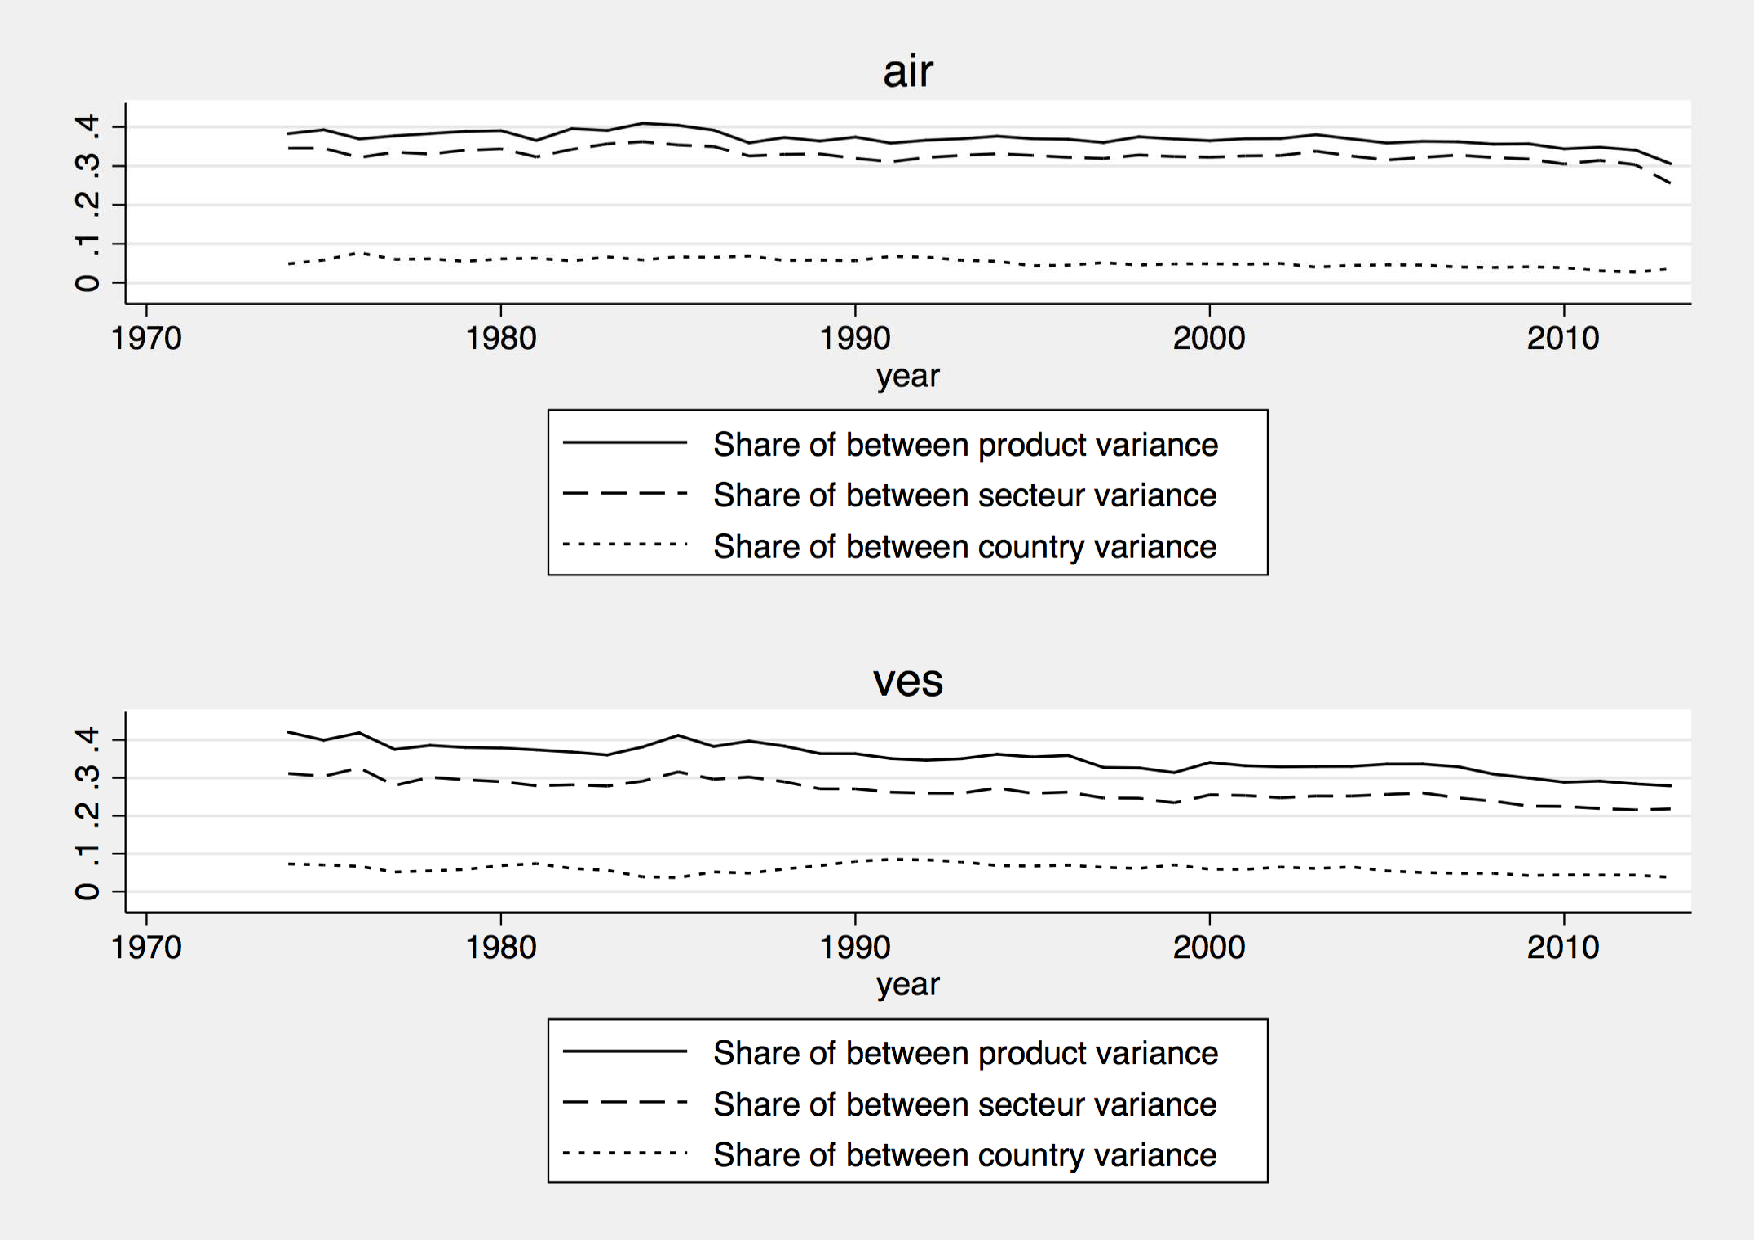
\includegraphics[width=10cm, height=7cm]{variance_decomposition.pdf}
%{\footnotesize {OECD data} }
\end{center}
\end{figure}


Two interesting results emerge from Figure \ref{fig:decomp_variance}.
First, the share of the cif-fas price gap variance that comes from the variance between products (5-digit level) is of the same magnitude of order as the variance between sectors at the 3-digit level.
Both account for between 30 and 40\% of the total variance in air transport, depending on the years considered.
This is also the case for vessel transport, even if the difference between the between-product variance share and the between-sector share is more pronounced (30\% for the between-sector vs 40\% for the between-product variance at the beginning of the period).
This provides an indirect robustness check to the degree of classification we have retained to estimate international transport costs.
Second, the variance of the cif-fas price gap that can be attributed to the product (or sector) dimension is much larger than the between-country variance.
This holds throughout the period and for both transport modes. By extension, one can expect a limited role of distance and other country-related variables as determinants of transport costs.


\setcounter{table}{0}
\renewcommand{\thetable}{C.\arabic{table}}

\setcounter{figure}{0}
\renewcommand{\thefigure}{C.\arabic{figure}}



\subsubsection{Separability Assumption}


This section reports two supplementary checks concerning the separability assumption.

\paragraph{Comparison on a yearly basis} We investigate this comparison deeper on a year-to-year basis, as shown in Figure \ref{fig:robustesse_non_separe}. Specifically, Figure \ref{fig:robustesse_non_separe} displays the results for air transport in panel (A) and for maritime transport in panel (B). In each case, the estimated values (as well as the fitted regression line) under both separability (baseline) and non-separability are reported, for the additive term (upper panel) and the ad-valorem term (lower panel).


\begin{figure}[htbp]
\caption{Robustness to the separability assumption (year-to-year basis)}
\label{fig:robustesse_non_separe}
\begin{center}
\begin{tabular}{cc}
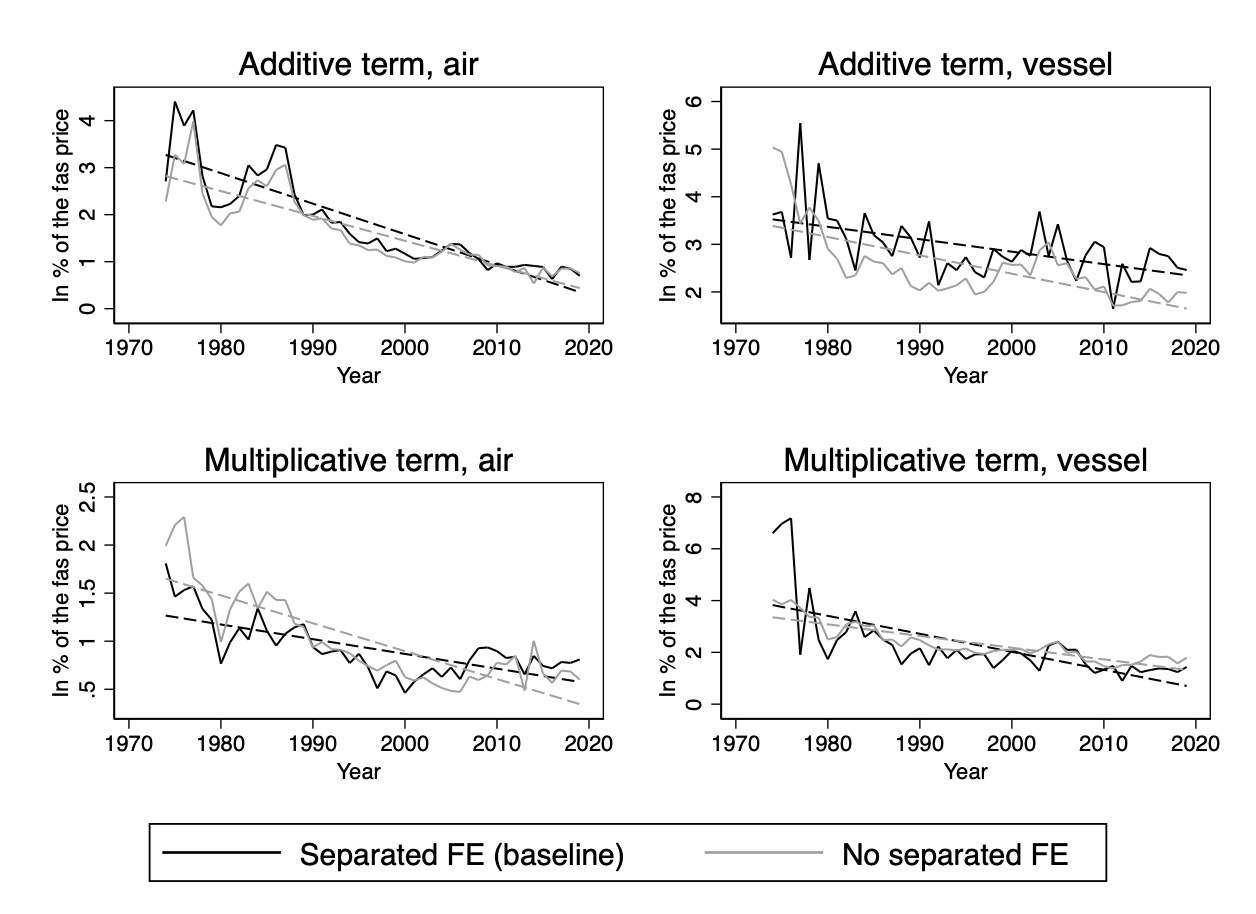
\includegraphics[width=6in, height=4in]{graph_robustesse_ns.jpg}

\end{tabular}
\end{center}
\begin{minipage} [c]  {5in} \scriptsize%
Notes: FE for (country, sector) fixed effects.
\end{minipage}
\end{figure}

In line with Table 2 of the paper, the results shown in Figure \ref{fig:robustesse_non_separe} confirm that the separability assumption (retained in our baseline estimation) tends to overestimate the value of the additive cost component (and underestimate the value of the ad-valorem cost).
However, they also show that the difference is quantitatively small in most cases. Further, and most importantly, whatever the transport mode and for both types of transport costs, the trend patterns of international transport costs, whether estimated under the separability assumption or not, are very similar. Along with the quality-of-fit diagnosis, this confirms the robustness of our estimation results to this assumption.


\paragraph{Distribution of the $\beta$} As final check, we also investigate whether the varying pattern over time/country of origin/product is also robust to the separability assumption. With this aim, we report in Figure \ref{fig:histogram_beta_robustness}
the histogram of the distribution of the elasticity of transport costs to the export price ($\beta_{ikt}$, for air transport (top panel) and for maritime transport (bottom panel) under the baseline specification (Panels (A), (c))) and the non-separability scenario (Panels (B), (c)).


\begin{figure}[htbp]
\caption{Histogram of the share of additive costs in total costs (restricted sample)}
\label{fig:histogram_beta_robustness}
\begin{center}
\begin{tabular}{cc}
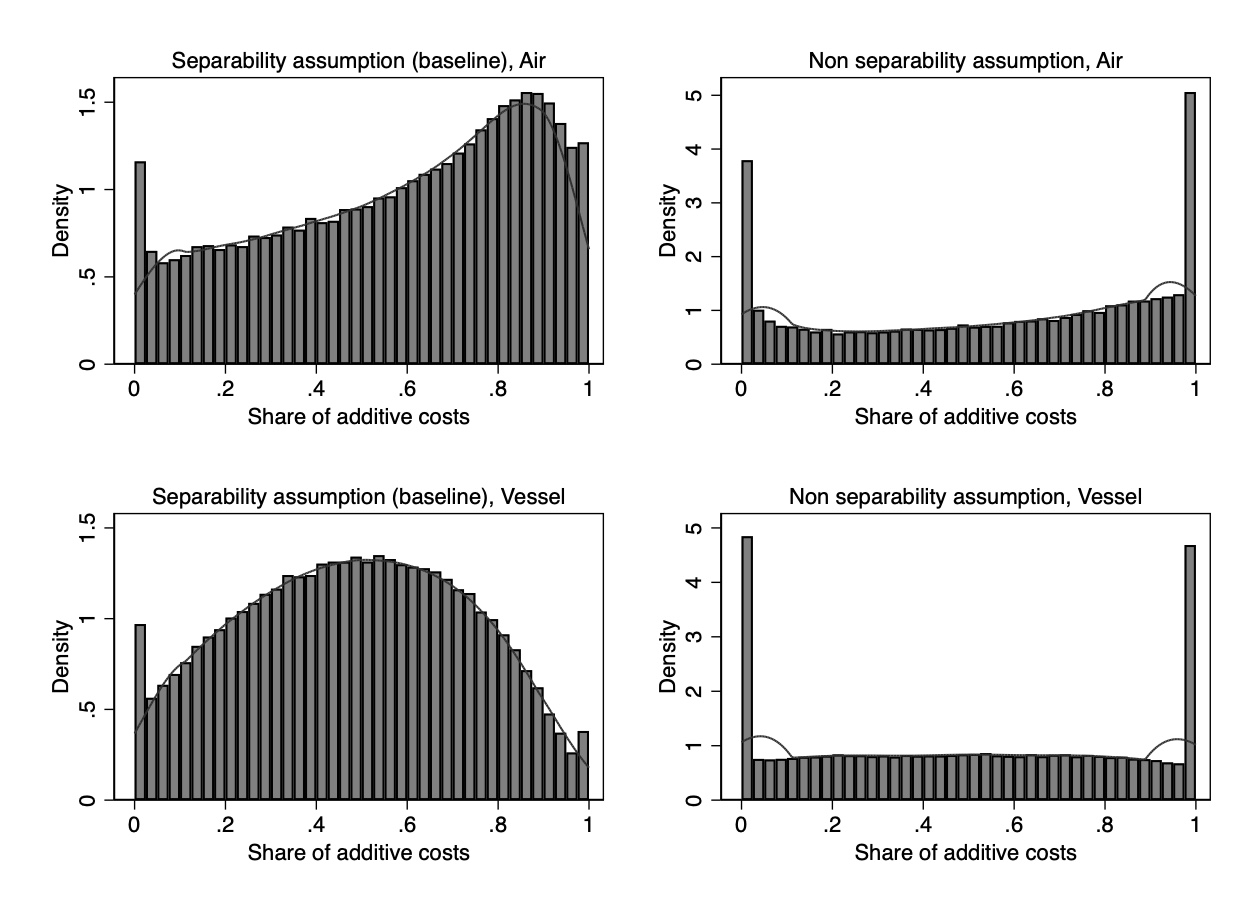
\includegraphics[width=14cm, height=10cm]{Etude_beta_pond.jpg}\\
\multicolumn{2}{l}{{\footnotesize Notes: Distribution of $\beta_{ikt}$ over the triplet (year-product-country), weighted by share of yearly value of flow.}}\\
\end{tabular}
\end{center}
\end{figure}

\textbf{Je ne comprends pas ce paragraphe. La footnote semble être ancienne. Mais en quoi est-ce que les histogrammes nous aident ? Éventuellement à dire qu’il y a moins de solutions de coin lorsqu’on fait l’estimation en séparé ? G.D.}For both transport modes the distribution of $\beta_{ikt}$ over the triplet (year, country of origin, product) appears smoothly distributed over the interval $[0,1]$, whatever the assumption regarding the specification of fixed effects.
Relaxing the assumption that fixed effects are separable between the two country and product dimensions does not alter qualitatively our conclusion, that the elasticity of transport costs to the export price (or the share of additive costs in total transport costs), is strongly varying over time, countries of origin and products.
\footnote{As a consequence, this also provides an indirect robustness check to the results regarding the trend decomposition provided in Section 4 of the paper, which establish that the decline of ``pure'' transport costs is a main reason for the decrease of overall transport costs observed over time.}



\subsubsection{Estimating $\widehat{\beta}_{i,s}$ directly}
	
In this section, we explore an alternative estimation method, which proceeds as follows. $\beta$ can be separately estimated for each industry $s$-origin country $i$ using the following regression:

\begin{equation}
\ln TC_{ikd} = \beta_{is}\ln \tilde{p}_{ikd} + Z_{ikd} +\epsilon_{ikd} \label{eq:estimation_ref1}
\end{equation}

where $d$ denotes the US district of entry and $k$ denotes an HS-10 product, $TC_{ikd}$ being the transport costs and $Z$ a set of controls variables. The identification of $\beta_{is}$, in this case, relies on exploiting the variability between sub-sectors at the 10-digit
level ($k$) and between ports of entry in the US ($d$). From this, one can then recover the levels of additive and multiplicative transports costs. Denoting $\widehat{\beta}_{is(k)}$ the estimated $\beta$ for a given sector-country $i,s(k)$, one can indeed solve the following two-equation system:

\begin{eqnarray*}
p_{ik} &=& \tau_{is(k)}\widetilde{p}_{ik} +t_{is(k)} \label{eq:system1}\\
\frac{t_{is(k)}}{(\tau_{is(k)}-1)\widetilde{p}_{ik}+ t_{is(k)}} &=& \widehat{\beta}_{is(k)}  \label{eq:system2}
\end{eqnarray*}


\noindent with $p_{ik}$ and $\widetilde{p}_{ik}$ the cif and fas prices observed in our dataset (conditional on a given year-transport mode).

One advantage of this approach is that the above regression can be estimated separately for various country-industry pairs on a linear basis, without having to resort on the separability assumption. This does not solve the issue yet, for two main reasons. First, it is still constrained to resort to non-linear estimators. This is due to the necessity of imposing an \textit{ex-ante} restriction on parameters, i.e. imposing $0 \leq  \beta \leq 1$. Should we relax this restriction, standard linear, least squares estimates often deliver negative, meaningless estimates. In this respect, implementing this does not suppress the requirement of resorting on non-linear estimates (and the computational, time-consuming burden it induces).

It should also be noted that this estimation method implies a lower coverage, both in time and in the sectors/countries covered. Information about the port of entry are only available since 1989, which is already smaller than our full sample starting in 1974. On top of that, because of the Covid situation, the US Bureau of Census was only able to send them the CDs relative to the years 1997-1999 and 2001-2019. Implementing the referee's method would hence necessarily reduce the time coverage of our analysis by more than 20 years (skipping the 1974-1996 years in particular). In our view, the historical coverage is interesting per se, as it provides useful insights about how transport costs have evolved over time.

With respect to the trade flows coverage, the method is run country by country, and 3-digit sector by 3-digit sector, exploiting the variability within each country-3d sector across 10-d sub-sectors and ports of entry. Yet, it appears that for many couples (country, 3-digit sector), there is too few variability across sub-sectors or ports en entry given the number of fixed effects included in the regression, such that estimation can not be run. This can be seen comparing the number of observations by year/ transport mode between this alternative method and our baseline method reported in Table \ref{tab_comp_referee1_baseline}. Put it differently, this methodology discards countries which export a limited range of goods to the US and/or which arrive in the USA through the same ports of entry. In this respect, the induced selection bias reduces the general scope of the transport costs estimates.

Notwithstanding these limitations, it remains interesting to run this alternative estimation method as robustness check. Table \ref{tab_comp_referee1_baseline} reports the estimation results, by transport mode, in the Column ``Alternative'', along with the results obtained with our baseline method over the same period 2005-2013. As noted above, the partners-sectors covered are lower. Regarding the share of additive costs $\beta$, the comparison between the two methods goes in opposite directions depending on the transport mode. While the estimated $\beta$ is lower for maritime transport with the alternative method (also displaying a larger decrease over the period), the opposite holds for Air transport. In any case yet, the share of additive costs remains substantial, around 40\% on average over the period, thereby confirming the main message of our paper shedding light on the importance of the additive component in international transport costs.


\begin{table}[htbp]
	\caption{Baseline and direct beta estimate 2005-2013}
	\begin{center}		
		\begin{tabular}{l|cc|cc}
\cline{1-5}
\multicolumn{1}{c}{Transport mode} &
  \multicolumn{2}{|c|}{Air} &
  \multicolumn{2}{c}{Vessel} \\ \hline
Estimation method &
Alternative &
Baseline &
Alternative &
Baseline \\ \hline
Coverage  \\ \hline
\hspace{1em}Nb sectors &
177 &
217 &
203 &
227 \\
\hspace{1em}Nb partners &
112 &
210 &
123 &
204 \\
\hspace{1em}Nb pairs &
3,872 &
12,158 &
3,743 &
12,440 \\ 
\hspace{1em}Annual covered value in Bn U.S. \$ &
262 &
293 &
824 &
906 \\ \hline
\multicolumn{5}{l}{Share of additive costs $\beta$}  \\ \hline
\hspace{1em}Mean &
0.39 &
0.25 &
0.45 &
0.50 \\
\hspace{1em}Median &
0.39 &
0.22 &
0.41 &
0.48 \\
\hspace{1em}Std. dev. &
0.15 &
0.19 &
0.29 &
0.28 \\
\hspace{1em}Time trend coefficient &
-0.012 &
-0.020 &
-0.012 &
-0.031 \\ \hline
%$\beta_{2005}$ &
%  0.41 &
%0.29 &
%0.46 &
%0.53 \\
%$\beta_{2013}$ &
%0.38 &
%0.27 &
%0.44 &
%0.33 \\
%\cline{1-5}
\end{tabular}

	
{\parbox[l]{12cm}{ \vspace{4pt}\footnotesize{Notes: Mean values reported for the 2005 and 2013 values reported for $\beta$. Time trend coefficient is the annual growth rate.}}}
\end{center}
	\label{tab_comp_referee1_baseline}%
\end{table}%

\begin{figure}[htbp]
	\caption{Baseline and direct beta estimate }
	\begin{center}
		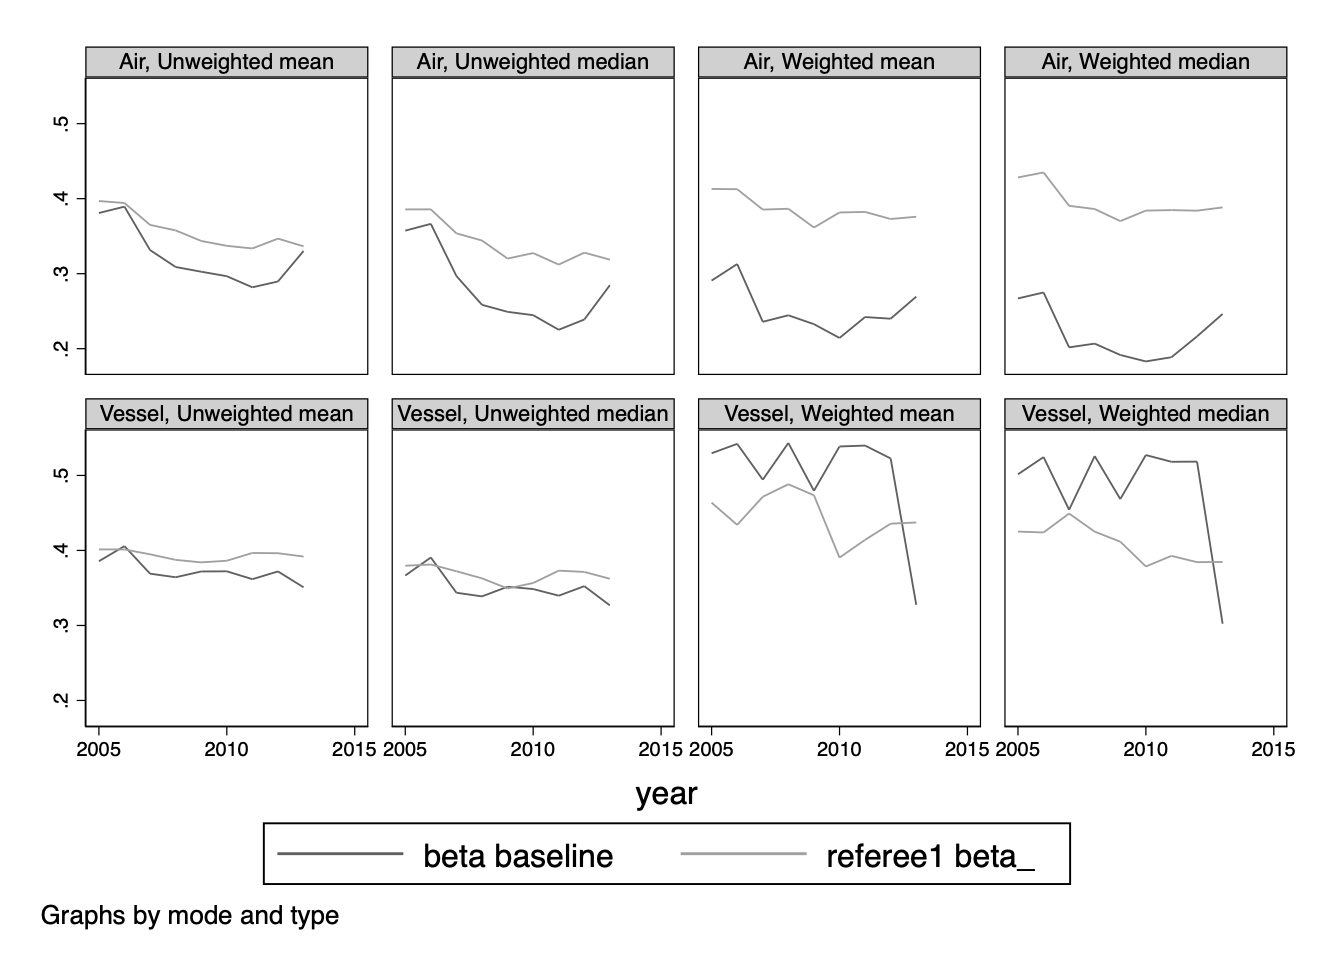
\includegraphics[height=8cm]
		{../scatter_chronology_baseline_referee1.png}
	\end{center}
\end{figure}


\subsubsection{Weights and quantities}


\begin{table}[htbp]
	\caption{Comparison 2005-2019, price per qy or price per kg}
	\begin{center}		
		\begin{tabular}{lllllll}
\cline{1-7}
\multicolumn{1}{c}{} &
  \multicolumn{3}{|c}{air} &
  \multicolumn{3}{c}{ves} \\
\multicolumn{1}{c}{} &
  \multicolumn{1}{|r}{hs10\_qy1\_qy} &
  \multicolumn{1}{r}{hs10\_qy1\_wgt} &
  \multicolumn{1}{r}{baseline} &
  \multicolumn{1}{r}{hs10\_qy1\_qy} &
  \multicolumn{1}{r}{hs10\_qy1\_wgt} &
  \multicolumn{1}{r}{baseline} \\
\cline{1-7}
\multicolumn{1}{l}{Mean} &
  \multicolumn{1}{|r}{} &
  \multicolumn{1}{r}{} &
  \multicolumn{1}{r}{} &
  \multicolumn{1}{r}{} &
  \multicolumn{1}{r}{} &
  \multicolumn{1}{r}{} \\
\multicolumn{1}{l}{\hspace{1em}Nb\_sectors} &
  \multicolumn{1}{|r}{216} &
  \multicolumn{1}{r}{217} &
  \multicolumn{1}{r}{217} &
  \multicolumn{1}{r}{223} &
  \multicolumn{1}{r}{226} &
  \multicolumn{1}{r}{226} \\
\multicolumn{1}{l}{\hspace{1em}Nb\_partners} &
  \multicolumn{1}{|r}{207} &
  \multicolumn{1}{r}{210} &
  \multicolumn{1}{r}{210} &
  \multicolumn{1}{r}{204} &
  \multicolumn{1}{r}{205} &
  \multicolumn{1}{r}{205} \\
\multicolumn{1}{l}{\hspace{1em}Nb\_pairs} &
  \multicolumn{1}{|r}{11,210} &
  \multicolumn{1}{r}{12,461} &
  \multicolumn{1}{r}{12,461} &
  \multicolumn{1}{r}{11,931} &
  \multicolumn{1}{r}{12,656} &
  \multicolumn{1}{r}{12,656} \\
\multicolumn{1}{l}{\hspace{1em}Covered trade value} &
  \multicolumn{1}{|r}{3.01e+11} &
  \multicolumn{1}{r}{3.23e+11} &
  \multicolumn{1}{r}{3.23e+11} &
  \multicolumn{1}{r}{8.98e+11} &
  \multicolumn{1}{r}{9.18e+11} &
  \multicolumn{1}{r}{9.18e+11} \\
\multicolumn{1}{l}{beta} &
  \multicolumn{1}{|r}{} &
  \multicolumn{1}{r}{} &
  \multicolumn{1}{r}{} &
  \multicolumn{1}{r}{} &
  \multicolumn{1}{r}{} &
  \multicolumn{1}{r}{} \\
\multicolumn{1}{l}{\hspace{1em}Mean} &
  \multicolumn{1}{|r}{0.05} &
  \multicolumn{1}{r}{0.23} &
  \multicolumn{1}{r}{0.23} &
  \multicolumn{1}{r}{0.21} &
  \multicolumn{1}{r}{0.45} &
  \multicolumn{1}{r}{0.47} \\
\multicolumn{1}{l}{\hspace{1em}Median} &
  \multicolumn{1}{|r}{0.00} &
  \multicolumn{1}{r}{0.18} &
  \multicolumn{1}{r}{0.19} &
  \multicolumn{1}{r}{0.05} &
  \multicolumn{1}{r}{0.44} &
  \multicolumn{1}{r}{0.45} \\
\multicolumn{1}{l}{\hspace{1em}Std. dev.} &
  \multicolumn{1}{|r}{0.12} &
  \multicolumn{1}{r}{0.20} &
  \multicolumn{1}{r}{0.19} &
  \multicolumn{1}{r}{0.28} &
  \multicolumn{1}{r}{0.25} &
  \multicolumn{1}{r}{0.27} \\
\multicolumn{1}{l}{Time trend} &
  \multicolumn{1}{|r}{} &
  \multicolumn{1}{r}{} &
  \multicolumn{1}{r}{} &
  \multicolumn{1}{r}{} &
  \multicolumn{1}{r}{} &
  \multicolumn{1}{r}{} \\
\multicolumn{1}{l}{\hspace{1em}Coefficient} &
  \multicolumn{1}{|r}{-0.073} &
  \multicolumn{1}{r}{-0.059} &
  \multicolumn{1}{r}{-0.061} &
  \multicolumn{1}{r}{-0.354} &
  \multicolumn{1}{r}{-0.059} &
  \multicolumn{1}{r}{-0.066} \\
\multicolumn{1}{l}{beta\_2005} &
  \multicolumn{1}{|r}{} &
  \multicolumn{1}{r}{} &
  \multicolumn{1}{r}{} &
  \multicolumn{1}{r}{} &
  \multicolumn{1}{r}{} &
  \multicolumn{1}{r}{} \\
\multicolumn{1}{l}{\hspace{1em}Mean} &
  \multicolumn{1}{|r}{0.04} &
  \multicolumn{1}{r}{0.30} &
  \multicolumn{1}{r}{0.29} &
  \multicolumn{1}{r}{0.27} &
  \multicolumn{1}{r}{0.50} &
  \multicolumn{1}{r}{0.53} \\
\multicolumn{1}{l}{beta\_2019} &
  \multicolumn{1}{|r}{} &
  \multicolumn{1}{r}{} &
  \multicolumn{1}{r}{} &
  \multicolumn{1}{r}{} &
  \multicolumn{1}{r}{} &
  \multicolumn{1}{r}{} \\
\multicolumn{1}{l}{\hspace{1em}Mean} &
  \multicolumn{1}{|r}{0.04} &
  \multicolumn{1}{r}{0.20} &
  \multicolumn{1}{r}{0.19} &
  \multicolumn{1}{r}{0.25} &
  \multicolumn{1}{r}{0.50} &
  \multicolumn{1}{r}{0.50} \\
\cline{1-7}
\end{tabular}

	\end{center}
	\label{tab_comp_referee1_baseline}%
\end{table}%




\begin{figure}[htbp]
	\caption{Comparison 2005-2019, price per qy or price per kg}
	\begin{center}
	\includegraphics[height=8cm]
	{../scatter_chronology_non_séparé_wgt_non_séparé_qy.png}
	\end{center}
\end{figure}

J’AI CHANGÉ LA DÉFINITION DU TIME TREND. JE FAIS MAINTENANT LE TREND ENTRE LES BETA MOYENS PAR ANNÉES AU LIEU D’UNE REGRESSIONS SUR TOUS LES BETAS PONDÉRÉ PAR LEUR PART DANS LE COMMERCE. GD.

\subsection{Eliminating the composition effects} \label{sec_oa:comp-effects}

\subsubsection{More on the Hummel's methodology}

This section complements Section 4 in the main paper, where we replicate the method adopted by \cite{hummels2007} on our database. Here, we report the unfitted measure of transport costs versus the ``pure'' transport costs series, i.e composition effects excluded
in percentage of the export price, as in \cite{hummels2007}. We also adopt Hummel's (2007) terminology, contrasting the ``expenditure/importe value'' (i.e, the unfitted serie) and the ``fitted ad-valorem rate'' (i.e, corresponding to the ``pure'' transport costs series, composition effects excluded). Unsurprisingly, this accords with his Figure 5 (for Air) and 6 (Vessel) for the comme period (until 2014).

\begin{figure}[htbp]
\caption{Characterizing the time trends: applying Hummel's (2007) method }
\label{fig:comp_effects_as_in_Hummels}
\begin{center}
\begin{tabular}{cc}
{\small (A) Ad-valorem air freight} & {\small (B) Ad-valorem vessel freight}\\
\multicolumn{2}{c}{{\small In percent of the export price}} \\
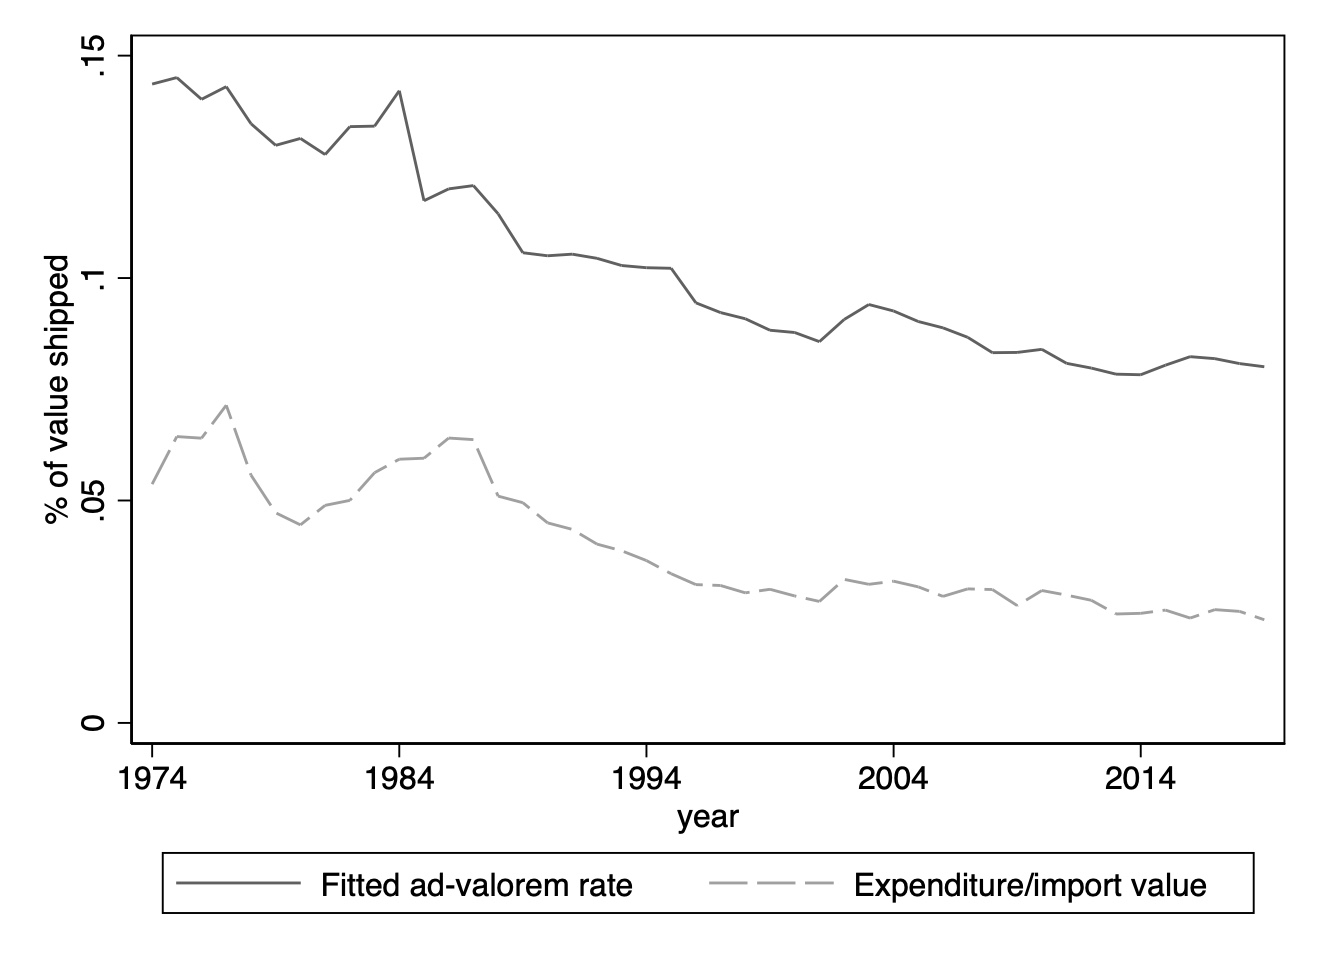
\includegraphics[width=2.5in, height=1.8in]{figure5_comme_hummels.jpg}
& 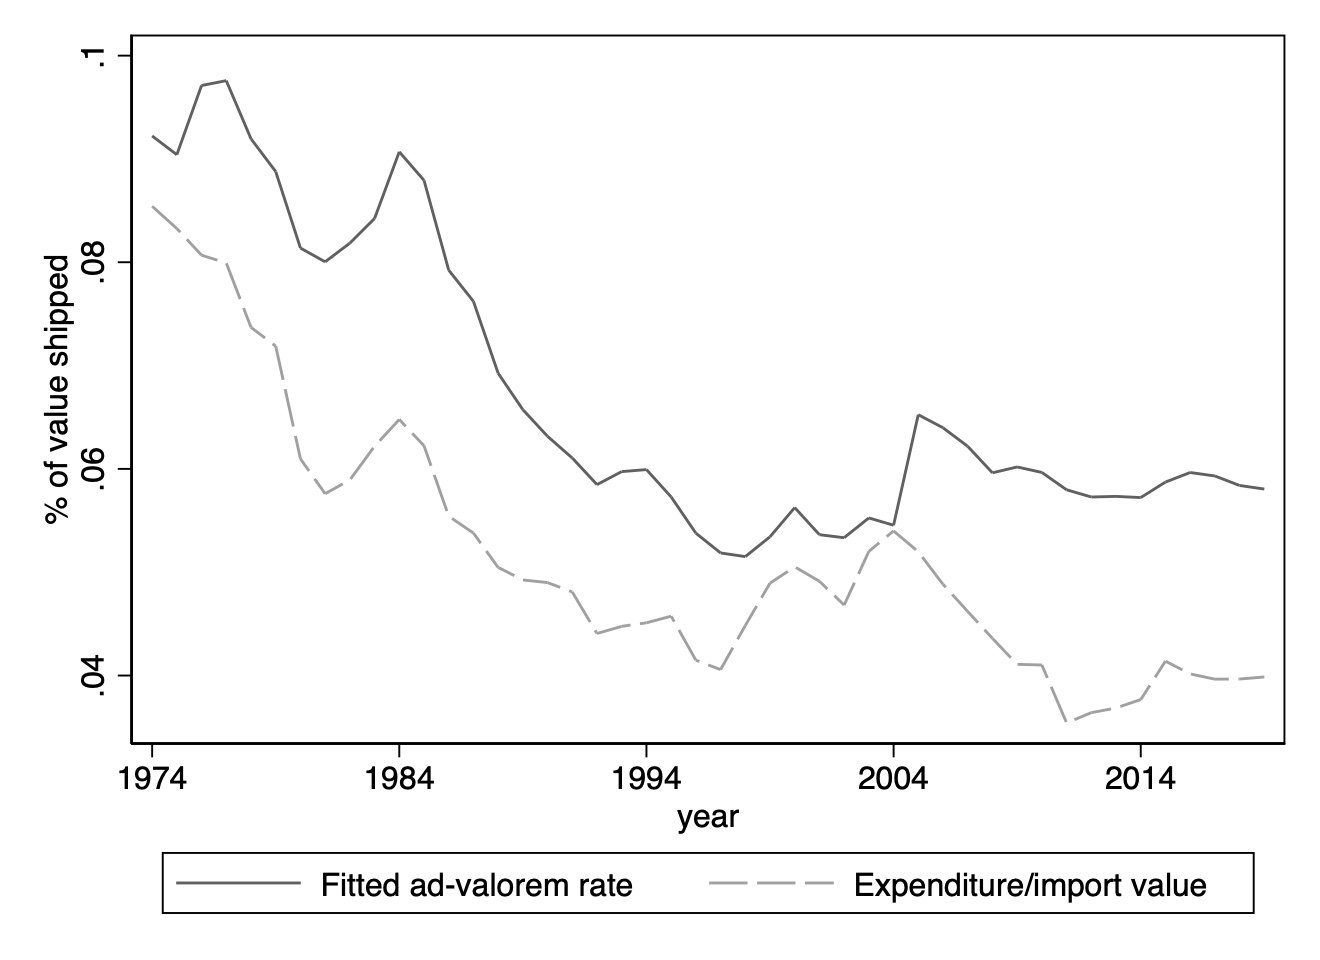
\includegraphics[width=2.5in,height=1.8in]{figure6_comme_hummels.jpg} \\
{\small (c) Ad-valorem air freight} & {\small (d) Ad-valorem vessel freight} \\
\end{tabular}
\end{center}
\end{figure}

\subsubsection{Composition effects: Primary vs. Manufacturing sector}
In this section, we refine the characterization of the evolution of international transport costs by distinguishing primary goods trade flows and and manufactured goods trade flows. The evolution in transport costs over time, by transport mode (overall transport costs and composition effects excluded) are reported in Figure \ref{fig:totalTC_compeffects_excl_manuf} for the manufacturing sector, and in Figure \ref{fig:totalTC_compeffects_excl_primary} for the primary goods. For easing comparison, we also report the results obtained on the whole range of trade flows (i.e., Figure 2 of the paper), in Figure \ref{fig:totalTC_compeffects_excl}.


The classification retained to categorize trade flows follows the UNCTAD classification (on STIC Revision 3)\footnote{See "UNCTAD product groupings and composition (SITC Rev. 3)" in http://unctadstat.unctad.org/EN/Classifications.html, accessed Septembre 2018}.
Are considered as ``primary goods'' all flows recorded as ``Food and live animals'' (First digit ``0'' in the SITC Classification), ``Beverages and tobacco'' (First digit ``1''), ``Crude materials, inedible, except fuels'' (First digit ``2''), ``Mineral fuels, lubricants and related materials'' (First digit ``3''), ``Animal and vegetable oils, fats and waxes'' (First digit ``4''), ``Pearls, precious \& semi-precious stones'' (Classified ``667'' in the SITC Classification) and ``Non-ferrous metals'' (classified ``68'' in the SITC Classification).


\begin{figure}[htbp]
\caption{Transport costs (with and without composition effects), Manufacturing}
\label{fig:totalTC_compeffects_excl_manuf}
\begin{center}
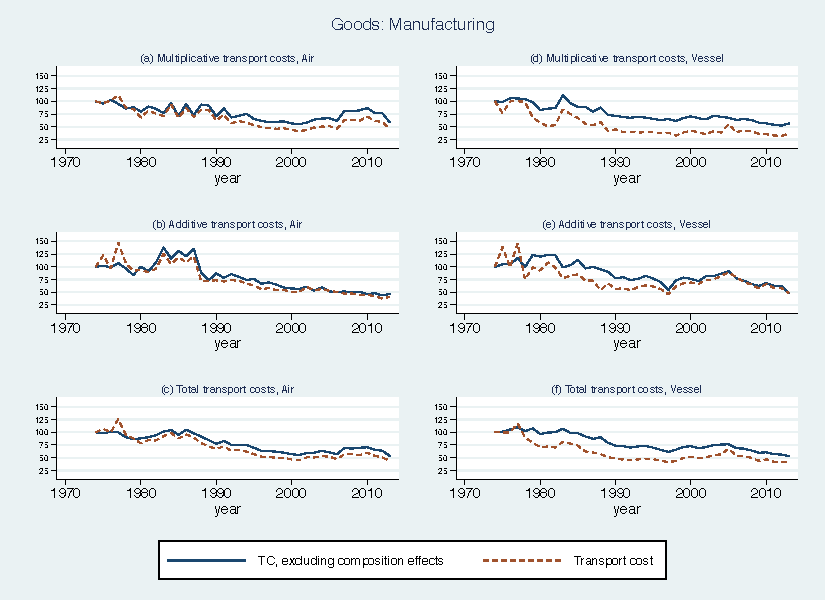
\includegraphics[height=8cm] {graph_composition_manuf.pdf}
\end{center}
\end{figure}

\begin{figure}[htbp]
\caption{Transport costs (with and without composition effects), Primary goods}
\label{fig:totalTC_compeffects_excl_primary}
\begin{center}
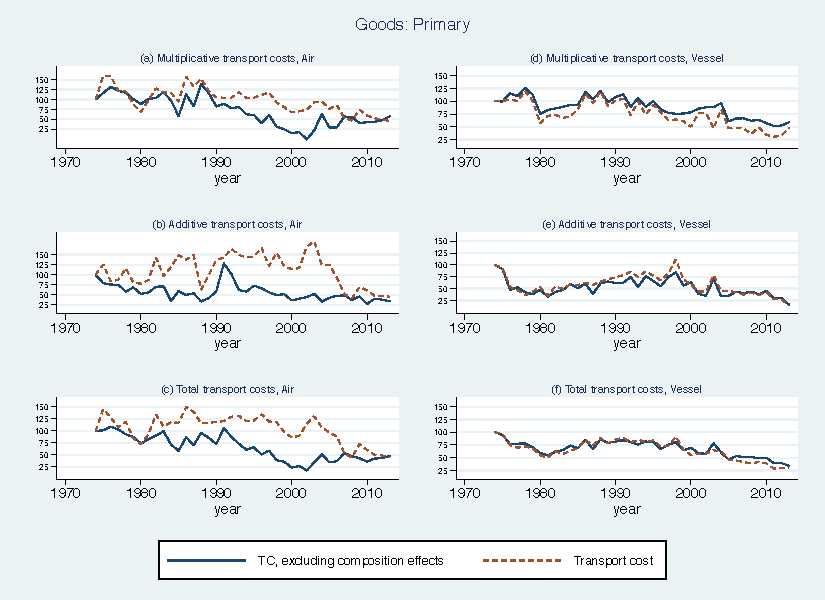
\includegraphics[height=8cm]
{graph_composition_primary.pdf}
\end{center}
\end{figure}

\begin{figure}[htbp]
\caption{Transport costs (with and without composition effects)}
\label{fig:totalTC_compeffects_excl}
\begin{center}
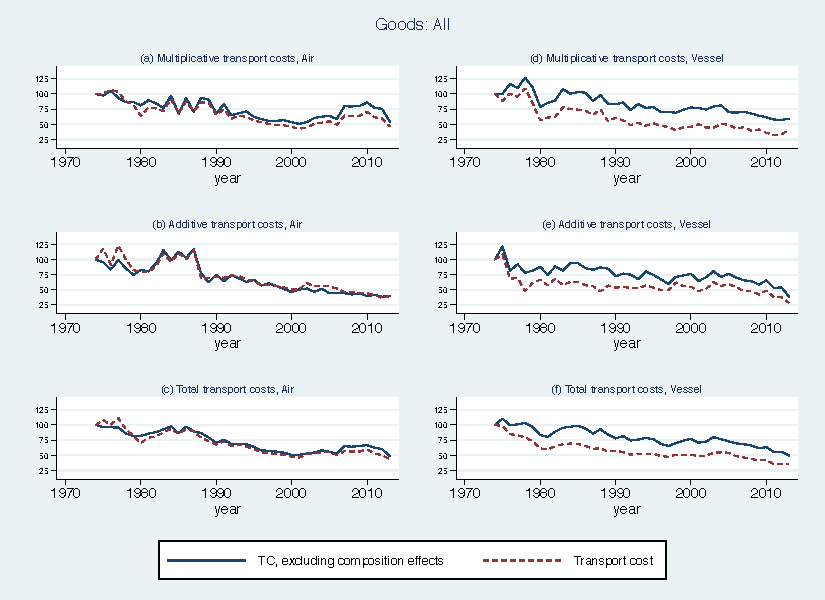
\includegraphics[height=8cm]
{graph_composition_all.pdf}
\end{center}
\end{figure}

As reported in Figures \ref{fig:totalTC_compeffects_excl_manuf} and \ref{fig:totalTC_compeffects_excl_primary}, both the ``pure'' transport costs and the unfitted measure, in the red dashed have regularly declined over the period in both sectors, by roughly the same order of magnitude (50\% in air, 60\% in vessel for overall transport costs, panels (c) and (f)). However the role of trade composition effects in accounting for this trend pattern differs depending on the sector.\\
In the manufacturing sector, Figure \ref{fig:totalTC_compeffects_excl_manuf}) reports a very similar time trend decomposition than what is obtained on the whole range of goods (Figure \ref{fig:totalTC_compeffects_excl}).  In air transport, most of the decrease can be imputed to the reduction of``ceteris paribus'' transport costs (the blue continuous line), trade composition effects playing virtually no role (Figure \ref{fig:totalTC_compeffects_excl_manuf}, left-hand panels (a), (b) and (c)). Trade composition effects matter more in vessel transport (Figure \ref{fig:totalTC_compeffects_excl_manuf}, right-hand panels (d), (e) and (f)), primarily in the ad-valorem component. As for the whole range of flows, the 60\% decrease in the unfitted transport costs in vessel can de decomposed in a 50\% decrease in the ``ceteris paribus'' transport costs (fitted), the 10\% remaining to trade composition effects.

The situation is strikingly different for primary goods only. In this case, it is in air transport that composition effects do matter (Figure \ref{fig:totalTC_compeffects_excl_primary}, left-hand panels (a), (b) and (c)), while we observe not much role for them in vessel transport (Figure \ref{fig:totalTC_compeffects_excl_primary}, left-hand panels (d), (e) and (f)). Furthermore, in air transport, composition effects matter by partially offsetting the decrease in the ``ceteris paribus'' transport costs (ie, implying a reduction in the ``raw'' transport costs over time much less pronounced than the fitted transport cost measures).

One explanation for the similarity between the results for the manufacturing goods trade and for total trade can be found in the share of primary goods in total flows as reported in Figure \ref{fig:Share_prim_goods}. In air transport, the share of primary goods in the total value of US imports is very small, around 10\%. Primary goods make a higher proportion of trade flows in vessel transport, especially over 1974-1982 (between 40\% and 60\%). On the following sub-period though, their share has fallen to 20-30\%. Given the modest proportion of primary goods in total import flows of the US economy compared to the manufactured sector, it is hence not surprising that the diagnosis made about the time trend of transport costs when all types of flows are considered is driven by the trend patterns that occur within the manufacturing sector.

\begin{figure}[htbp]
\caption{Share of primary goods in the value of total US imports}
\label{fig:Share_prim_goods}
\begin{center}
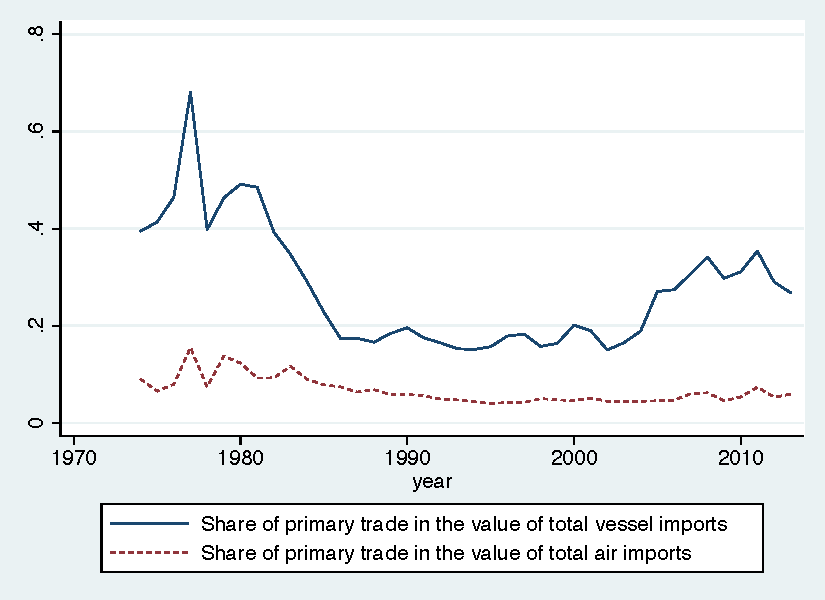
\includegraphics[height=6cm]
{Share_of_primary.pdf}
\end{center}
\end{figure}



\end{document}
